\documentclass[twoside]{book}

% Packages required by doxygen
\usepackage{fixltx2e}
\usepackage{calc}
\usepackage{doxygen}
\usepackage[export]{adjustbox} % also loads graphicx
\usepackage{graphicx}
\usepackage[utf8]{inputenc}
\usepackage{makeidx}
\usepackage{multicol}
\usepackage{multirow}
\PassOptionsToPackage{warn}{textcomp}
\usepackage{textcomp}
\usepackage[nointegrals]{wasysym}
\usepackage[table]{xcolor}

% NLS support packages
\usepackage[T2A]{fontenc}
\usepackage[russian]{babel}

% Font selection
\usepackage[T1]{fontenc}
\usepackage[scaled=.90]{helvet}
\usepackage{courier}
\usepackage{amssymb}
\usepackage{sectsty}
\renewcommand{\familydefault}{\sfdefault}
\allsectionsfont{%
  \fontseries{bc}\selectfont%
  \color{darkgray}%
}
\renewcommand{\DoxyLabelFont}{%
  \fontseries{bc}\selectfont%
  \color{darkgray}%
}
\newcommand{\+}{\discretionary{\mbox{\scriptsize$\hookleftarrow$}}{}{}}

% Page & text layout
\usepackage{geometry}
\geometry{%
  a4paper,%
  top=2.5cm,%
  bottom=2.5cm,%
  left=2.5cm,%
  right=2.5cm%
}
\tolerance=750
\hfuzz=15pt
\hbadness=750
\setlength{\emergencystretch}{15pt}
\setlength{\parindent}{0cm}
\setlength{\parskip}{3ex plus 2ex minus 2ex}
\makeatletter
\renewcommand{\paragraph}{%
  \@startsection{paragraph}{4}{0ex}{-1.0ex}{1.0ex}{%
    \normalfont\normalsize\bfseries\SS@parafont%
  }%
}
\renewcommand{\subparagraph}{%
  \@startsection{subparagraph}{5}{0ex}{-1.0ex}{1.0ex}{%
    \normalfont\normalsize\bfseries\SS@subparafont%
  }%
}
\makeatother

% Headers & footers
\usepackage{fancyhdr}
\pagestyle{fancyplain}
\fancyhead[LE]{\fancyplain{}{\bfseries\thepage}}
\fancyhead[CE]{\fancyplain{}{}}
\fancyhead[RE]{\fancyplain{}{\bfseries\leftmark}}
\fancyhead[LO]{\fancyplain{}{\bfseries\rightmark}}
\fancyhead[CO]{\fancyplain{}{}}
\fancyhead[RO]{\fancyplain{}{\bfseries\thepage}}
\fancyfoot[LE]{\fancyplain{}{}}
\fancyfoot[CE]{\fancyplain{}{}}
\fancyfoot[RE]{\fancyplain{}{\bfseries\scriptsize Создано системой Doxygen }}
\fancyfoot[LO]{\fancyplain{}{\bfseries\scriptsize Создано системой Doxygen }}
\fancyfoot[CO]{\fancyplain{}{}}
\fancyfoot[RO]{\fancyplain{}{}}
\renewcommand{\footrulewidth}{0.4pt}
\renewcommand{\chaptermark}[1]{%
  \markboth{#1}{}%
}
\renewcommand{\sectionmark}[1]{%
  \markright{\thesection\ #1}%
}

% Indices & bibliography
\usepackage{natbib}
\usepackage[titles]{tocloft}
\setcounter{tocdepth}{3}
\setcounter{secnumdepth}{5}
\makeindex

% Hyperlinks (required, but should be loaded last)
\usepackage{ifpdf}
\ifpdf
  \usepackage[pdftex,pagebackref=true]{hyperref}
\else
  \usepackage[ps2pdf,pagebackref=true]{hyperref}
\fi
\hypersetup{%
  colorlinks=true,%
  linkcolor=blue,%
  citecolor=blue,%
  unicode%
}

% Custom commands
\newcommand{\clearemptydoublepage}{%
  \newpage{\pagestyle{empty}\cleardoublepage}%
}

\usepackage{caption}
\captionsetup{labelsep=space,justification=centering,font={bf},singlelinecheck=off,skip=4pt,position=top}

%===== C O N T E N T S =====

\begin{document}

% Titlepage & ToC
\hypersetup{pageanchor=false,
             bookmarksnumbered=true,
             pdfencoding=unicode
            }
\pagenumbering{alph}
\begin{titlepage}
\vspace*{7cm}
\begin{center}%
{\Large Logic Calculator }\\
\vspace*{1cm}
{\large Создано системой Doxygen 1.8.13}\\
\end{center}
\end{titlepage}
\clearemptydoublepage
\pagenumbering{roman}
\tableofcontents
\clearemptydoublepage
\pagenumbering{arabic}
\hypersetup{pageanchor=true}

%--- Begin generated contents ---
\chapter{Логический калькулятор}
\label{index}\hypertarget{index}{}На данный момент логический калькулятор умеет выполнять следующее\+:
\begin{DoxyItemize}
\item Ввод и проверка переменных на корректность. Под корректностью подразумевается правильное написание букв и операций над ними
\item Вывод таблицы истинности для выражения
\item СКНФ и СДНФ
\end{DoxyItemize}\hypertarget{index_autotoc_md7}{}\doxysection{Примеры выражений}\label{index_autotoc_md7}
\begin{DoxyVerb}A * B + C -> A
A * ( B + ( C -> ! A ) + B * C )
A * B + C -> ( D | A # B <- C ) ^ ! D ~ A
\end{DoxyVerb}
\hypertarget{index_autotoc_md8}{}\doxysection{Скачивание}\label{index_autotoc_md8}
Вы можете скачать \href{https://github.com/mvngr/logic_calculator/releases/download/1.3/LogicCalc_bin_win_amd64.zip}{\texttt{ бинарные файлы для Windows 7-\/10 x64}}\hypertarget{index_autotoc_md9}{}\doxysection{Описание классов}\label{index_autotoc_md9}
Полное описание методов и классов вы можете найти в документации к проекту -\/ \href{https://mvngr.github.io/logic_calculator_doc/html/index.html}{\texttt{ https\+://mvngr.\+github.\+io/logic\+\_\+calculator\+\_\+doc/html/index.\+html}}\hypertarget{index_autotoc_md10}{}\doxysection{Условные обозначения}\label{index_autotoc_md10}
Для корректной работы программы после каждого значащего значения нужно ставить пробел. Возможно, это будет поправлено в будущих версиях программы

Так же вы можете пользоваться скобками в своих задачах {\ttfamily ( )}\hypertarget{index_autotoc_md11}{}\doxysection{Операции}\label{index_autotoc_md11}
\tabulinesep=1mm
\begin{longtabu}spread 0pt [c]{*{2}{|X[-1]}|}
\hline
\PBS\centering \cellcolor{\tableheadbgcolor}\textbf{ Условное обозначение }&\PBS\centering \cellcolor{\tableheadbgcolor}\textbf{ Название операции  }\\\cline{1-2}
\endfirsthead
\hline
\endfoot
\hline
\PBS\centering \cellcolor{\tableheadbgcolor}\textbf{ Условное обозначение }&\PBS\centering \cellcolor{\tableheadbgcolor}\textbf{ Название операции  }\\\cline{1-2}
\endhead
\&\#42; &Конъюнкция  \\\cline{1-2}
\&\#43; &Дизъюнкция  \\\cline{1-2}
-\/$>$ &Импликация  \\\cline{1-2}
$<$-\/ &Обратная импликация  \\\cline{1-2}
\&\#448; &Штрих Шеффера  \\\cline{1-2}
\multirow{2}{*}{\&\#35; }&Стрелка Пирса  \\\cline{2-2}
&Исключающее ИЛИ  \\\cline{1-2}
$\sim$ &Эквиваленция  \\\cline{1-2}
! &Отрицание самой переменной  \\\cline{1-2}
\end{longtabu}
\hypertarget{index_autotoc_md12}{}\doxysection{Переменные}\label{index_autotoc_md12}
Для логических переменных была выделена только часть алфавита. Все возможные переменные\+:

{\ttfamily A B C D E F G X Y Z}

{\ttfamily a b c d e f g x y z}

Стоит помнить, что регистр учитывается\hypertarget{index_autotoc_md13}{}\doxysection{Скриншоты}\label{index_autotoc_md13}
  
\chapter{Старая версия документации}
\label{md__home_itain__qt_projects_logic_calculator_old_documentation}
\Hypertarget{md__home_itain__qt_projects_logic_calculator_old_documentation}
Классы, методы и переменные, которые использует калькулятор

\subsubsection*{\hyperlink{class_main_window}{Main\+Window}}

Класс отвечает за взаимодействие с пользовательским интерфейсом

\tabulinesep=1mm
\begin{longtabu} spread 0pt [c]{*{2}{|X[-1]}|}
\hline
\rowcolor{\tableheadbgcolor}\textbf{ Метод }&\textbf{ Описание  }\\\cline{1-2}
\endfirsthead
\hline
\endfoot
\hline
\rowcolor{\tableheadbgcolor}\textbf{ Метод }&\textbf{ Описание  }\\\cline{1-2}
\endhead
input\+Pressed &Обработчик для поля ввода данных, вызывается при нажатии на {\ttfamily enter} \\\cline{1-2}
on\+Clicked &Обработчик на кнопки логических операций. Добавляет в поле ввода данных соответствующий символ \\\cline{1-2}
bind\+Connect &Создаёт связи между обработчиком события {\ttfamily on\+Clicked} и нажатой кнопкой \\\cline{1-2}
on\+\_\+compute\+\_\+clicked &Обработчик нажатия на кнопку {\ttfamily Вычислить} \\\cline{1-2}
connect\+Qss &Отвечает за подключение стилей \\\cline{1-2}
on\+\_\+f4\+\_\+clicked &Обработчик для кнопки {\ttfamily СДНФ} \\\cline{1-2}
on\+\_\+f5\+\_\+clicked &Обработчик для кнопки {\ttfamily СКНФ} \\\cline{1-2}
\end{longtabu}
\subsubsection*{\hyperlink{class_input_editor}{Input\+Editor}}

Класс отвечает за обработку данных, вводимых в поле ввода данных

\tabulinesep=1mm
\begin{longtabu} spread 0pt [c]{*{2}{|X[-1]}|}
\hline
\rowcolor{\tableheadbgcolor}\textbf{ Переменная }&\textbf{ Описание  }\\\cline{1-2}
\endfirsthead
\hline
\endfoot
\hline
\rowcolor{\tableheadbgcolor}\textbf{ Переменная }&\textbf{ Описание  }\\\cline{1-2}
\endhead
input\+\_\+ &Используется для управления полем ввода данных \\\cline{1-2}
v\+\_\+ &Внутренний массив для хранения данных из поля ввода данных \\\cline{1-2}
\end{longtabu}
\tabulinesep=1mm
\begin{longtabu} spread 0pt [c]{*{2}{|X[-1]}|}
\hline
\rowcolor{\tableheadbgcolor}\textbf{ Метод }&\textbf{ Описание  }\\\cline{1-2}
\endfirsthead
\hline
\endfoot
\hline
\rowcolor{\tableheadbgcolor}\textbf{ Метод }&\textbf{ Описание  }\\\cline{1-2}
\endhead
Push\+Back &Добавляет определенные данные в конец внутреннего массива \\\cline{1-2}
to\+String &Преобразует внутренний массив в строку \\\cline{1-2}
parse &Парсит введенную строку, возвращает в виде переменной ответ, смогло ли произойти чтение \\\cline{1-2}
get\+Vars &Добавление в внутренний массив внешние данные \\\cline{1-2}
update\+Input &Обновляет поле для ввода данных \\\cline{1-2}
fill\+Consts &Заполняет словари заранее подготовленными данными \\\cline{1-2}
is\+Validity &Определяет корректность данных в внутреннем массиве относительно поля ввода данных \\\cline{1-2}
\end{longtabu}
\subsubsection*{\hyperlink{class_logic}{Logic}}

Класс отвечает за логику выполнения действий

\tabulinesep=1mm
\begin{longtabu} spread 0pt [c]{*{2}{|X[-1]}|}
\hline
\rowcolor{\tableheadbgcolor}\textbf{ Переменная }&\textbf{ Описание  }\\\cline{1-2}
\endfirsthead
\hline
\endfoot
\hline
\rowcolor{\tableheadbgcolor}\textbf{ Переменная }&\textbf{ Описание  }\\\cline{1-2}
\endhead
B\+I\+N\+A\+R\+Y\+\_\+\+O\+P\+E\+R\+A\+T\+I\+O\+N\+S\+\_\+ &Словарь бинарных операций \\\cline{1-2}
B\+I\+N\+A\+R\+Y\+\_\+\+O\+P\+E\+R\+A\+T\+I\+O\+N\+S\+\_\+\+T\+O\+\_\+\+N\+U\+M\+\_\+ &Сопоставление бинарной операции с её внутренним номером (нужно для удобства) \\\cline{1-2}
A\+V\+I\+A\+B\+L\+E\+\_\+\+N\+A\+M\+E\+\_\+\+O\+F\+\_\+\+V\+A\+R\+S\+\_\+ &Словарь разрешенных имен для логических переменных \\\cline{1-2}
vars\+\_\+ &Массив логических переменных \\\cline{1-2}
v\+\_\+ &Массив строк, разделенных при помощи пробела. Пример\+: {\ttfamily \{\char`\"{}\+A\char`\"{}, \char`\"{}$\ast$\char`\"{}, \char`\"{}\+B\char`\"{}, \char`\"{}+\char`\"{}, \char`\"{}!\char`\"{}, \char`\"{}\+C\char`\"{}\}} \\\cline{1-2}
map\+\_\+ &Используется для сопоставления строковых переменных и их аналогов из vars\+\_\+. {\ttfamily $<$Название переменной$>$ =$>$ $<$Индекс в массиве объекта$>$} \\\cline{1-2}
ce\+\_\+ &Используется для управление полем вывода \\\cline{1-2}
\end{longtabu}


\tabulinesep=1mm
\begin{longtabu} spread 0pt [c]{*{2}{|X[-1]}|}
\hline
\rowcolor{\tableheadbgcolor}\textbf{ Метод }&\textbf{ Описание  }\\\cline{1-2}
\endfirsthead
\hline
\endfoot
\hline
\rowcolor{\tableheadbgcolor}\textbf{ Метод }&\textbf{ Описание  }\\\cline{1-2}
\endhead
set\+Vars &Добавляет массив логических переменных в внутренний массив \\\cline{1-2}
compute &Инициирует вычисления \\\cline{1-2}
compute\+Logical\+Action &Инициирует вычисление таблицы истинности \\\cline{1-2}
get\+Vars\+Title &Отдает массив имен логических переменных \\\cline{1-2}
get\+Vars\+Data &Отдает массив всех данных из логических переменных \\\cline{1-2}
negation &Используется для выполнения отрицания у всей входной строки \\\cline{1-2}
negation\+Func &Используется для выполнения отрицания у выражений со скобками во входной строке \\\cline{1-2}
binary\+Operation &Используется для выполнения входной операции у всей входной строки \\\cline{1-2}
fill\+Operations &Используется для заполнения словарей \\\cline{1-2}
show\+Error &Выводит в пользовательский интерфейс сообщения с ошибками \\\cline{1-2}
insert\+With\+Replace &Выполняет внедрение логической операции в внутренние массивы взамен переменным(ой) и оператора \\\cline{1-2}
fill\+Vars &Добавляет логические переменные в vars\+\_\+ из строк {\ttfamily v\+\_\+} \\\cline{1-2}
fill\+Map &Заполняет карту {\ttfamily map\+\_\+} \\\cline{1-2}
is\+Repeat &Проверяет на повторение названия имен в {\ttfamily vars\+\_\+} \\\cline{1-2}
sort\+Vars &Сортирует массив {\ttfamily vars\+\_\+} по названиям \\\cline{1-2}
make\+Bool\+Arrays &Создает массив начальных данных у переменных \\\cline{1-2}
find\+Brackets &Находит выражения в скобках и высчитывает их \\\cline{1-2}
sub\+String &Возвращает подстроку из строки \\\cline{1-2}
make\+S\+K\+NF &создает Совершенную Конъюнктивную Нормальную Форму \\\cline{1-2}
make\+S\+D\+NF &создает Совершенную Дизъюнктивную Нормальную Форму \\\cline{1-2}
\end{longtabu}


\subsubsection*{\hyperlink{class_content_editor}{Content\+Editor}}

Класс отвечает за корректный и удобный вывод чего-\/либо в поле для вывода

\tabulinesep=1mm
\begin{longtabu} spread 0pt [c]{*{2}{|X[-1]}|}
\hline
\rowcolor{\tableheadbgcolor}\textbf{ Переменная }&\textbf{ Описание  }\\\cline{1-2}
\endfirsthead
\hline
\endfoot
\hline
\rowcolor{\tableheadbgcolor}\textbf{ Переменная }&\textbf{ Описание  }\\\cline{1-2}
\endhead
pte\+\_\+ &Управление полем вывода \\\cline{1-2}
cell\+Size\+\_\+ &Размеры ячеек в таблице истинности \\\cline{1-2}
\end{longtabu}
\tabulinesep=1mm
\begin{longtabu} spread 0pt [c]{*{2}{|X[-1]}|}
\hline
\rowcolor{\tableheadbgcolor}\textbf{ Метод }&\textbf{ Описание  }\\\cline{1-2}
\endfirsthead
\hline
\endfoot
\hline
\rowcolor{\tableheadbgcolor}\textbf{ Метод }&\textbf{ Описание  }\\\cline{1-2}
\endhead
print\+Truth\+Table &Инициирует вывод таблицы истинности \\\cline{1-2}
get\+Size &Заполняет значения размеров ячеек в таблице истинности {\ttfamily cell\+Size\+\_\+} \\\cline{1-2}
make\+String &Создает строку из повторяющихся amount раз символов segment \\\cline{1-2}
make\+Line &Создает линию под заголовком \\\cline{1-2}
make\+Title &Создает заголовок \\\cline{1-2}
make\+Data &Создает двумерный массив данных {\ttfamily $<$0/1$>$} \\\cline{1-2}
center\+Align &выравнивает все элементы по центру своей ячейки \\\cline{1-2}
print\+S\+K\+NF &выводит Совершенную Конъюнктивную Нормальную Форму \\\cline{1-2}
print\+S\+D\+NF &выводит Совершенную Дизъюнктивную Нормальную Форму \\\cline{1-2}
\end{longtabu}
\subsubsection*{\hyperlink{class_variable}{Variable}}

Класс логических переменных

\tabulinesep=1mm
\begin{longtabu} spread 0pt [c]{*{2}{|X[-1]}|}
\hline
\rowcolor{\tableheadbgcolor}\textbf{ Переменная }&\textbf{ Описание  }\\\cline{1-2}
\endfirsthead
\hline
\endfoot
\hline
\rowcolor{\tableheadbgcolor}\textbf{ Переменная }&\textbf{ Описание  }\\\cline{1-2}
\endhead
name\+\_\+ &Имя логической переменной \\\cline{1-2}
vars\+\_\+ &Принимаемые значения \\\cline{1-2}
\end{longtabu}
\tabulinesep=1mm
\begin{longtabu} spread 0pt [c]{*{2}{|X[-1]}|}
\hline
\rowcolor{\tableheadbgcolor}\textbf{ Метод }&\textbf{ Описание  }\\\cline{1-2}
\endfirsthead
\hline
\endfoot
\hline
\rowcolor{\tableheadbgcolor}\textbf{ Метод }&\textbf{ Описание  }\\\cline{1-2}
\endhead
conjunction &Конъюнкция с переменной {\ttfamily other} \\\cline{1-2}
disjunction &Дизъюнкция с переменной {\ttfamily other} \\\cline{1-2}
implication &Импликация с переменной {\ttfamily other} \\\cline{1-2}
converse &Обратная импликация с переменной {\ttfamily other} \\\cline{1-2}
not\+And &Штрих Шеффера с переменной {\ttfamily other} \\\cline{1-2}
not\+Or &Стрелка Пирса с переменной {\ttfamily other} \\\cline{1-2}
exclusive\+Disjunction &Исключающее ИЛИ с переменной {\ttfamily other} \\\cline{1-2}
equivalent &Эквиваленция с переменной {\ttfamily other} \\\cline{1-2}
negation &Отрицание самой переменной \\\cline{1-2}
set\+Name &Задает имя {\ttfamily name\+\_\+} как у переменной {\ttfamily name} \\\cline{1-2}
set\+Vars &Задает принимаемые значения {\ttfamily vars\+\_\+} как у массива {\ttfamily vars}, либо генерирует их, основываясь на индексе элемента и количестве элементов \\\cline{1-2}
get\+Name &Отдает значение {\ttfamily name\+\_\+} \\\cline{1-2}
get\+Vars &Отдает значение {\ttfamily vars\+\_\+} \\\cline{1-2}
debug\+Vars &Выводит значения {\ttfamily vars\+\_\+} в консоль (Не используется) \\\cline{1-2}
pow2 &Возвращает степень числа два \\\cline{1-2}
make\+Name &Создает строку из двух названий переменных и операции между ними \\\cline{1-2}
\end{longtabu}

\chapter{Алфавитный указатель пространств имен}
\section{Пространства имен}
Полный список пространств имен.\begin{DoxyCompactList}
\item\contentsline{section}{\hyperlink{namespace_ui}{Ui} }{\pageref{namespace_ui}}{}
\end{DoxyCompactList}

\chapter{Иерархический список классов}
\section{Иерархия классов}
Иерархия классов.\begin{DoxyCompactList}
\item \contentsline{section}{Content\+Editor}{\pageref{class_content_editor}}{}
\item \contentsline{section}{Input\+Editor}{\pageref{class_input_editor}}{}
\item \contentsline{section}{Logic}{\pageref{class_logic}}{}
\item Q\+Main\+Window\begin{DoxyCompactList}
\item \contentsline{section}{Main\+Window}{\pageref{class_main_window}}{}
\end{DoxyCompactList}
\item \contentsline{section}{Variable}{\pageref{class_variable}}{}
\end{DoxyCompactList}

\chapter{Алфавитный указатель классов}
\doxysection{Классы}
Классы с их кратким описанием.\begin{DoxyCompactList}
\item\contentsline{section}{\mbox{\hyperlink{class_content_editor}{Content\+Editor}} \\*\mbox{\hyperlink{class_content_editor}{Content\+Editor}} -\/ Класс отвечает за корректный и удобный вывод чего-\/либо в поле для вывода }{\pageref{class_content_editor}}{}
\item\contentsline{section}{\mbox{\hyperlink{class_input_editor}{Input\+Editor}} \\*\mbox{\hyperlink{class_input_editor}{Input\+Editor}} -\/ Класс отвечает за обработку данных, вводимых в поле ввода данных }{\pageref{class_input_editor}}{}
\item\contentsline{section}{\mbox{\hyperlink{class_logic}{Logic}} \\*\mbox{\hyperlink{class_logic}{Logic}} -\/ Класс отвечает за логику выполнения действий }{\pageref{class_logic}}{}
\item\contentsline{section}{\mbox{\hyperlink{class_main_window}{Main\+Window}} \\*\mbox{\hyperlink{class_main_window}{Main\+Window}} -\/ Класс отвечает за взаимодействие с пользовательским интерфейсом }{\pageref{class_main_window}}{}
\item\contentsline{section}{\mbox{\hyperlink{class_variable}{Variable}} \\*\mbox{\hyperlink{class_variable}{Variable}} -\/ Класс логических переменных }{\pageref{class_variable}}{}
\end{DoxyCompactList}

\chapter{Список файлов}
\doxysection{Файлы}
Полный список файлов.\begin{DoxyCompactList}
\item\contentsline{section}{/home/mike/projects/logic\+\_\+calculator/\mbox{\hyperlink{contenteditor_8cpp}{contenteditor.\+cpp}} }{\pageref{contenteditor_8cpp}}{}
\item\contentsline{section}{/home/mike/projects/logic\+\_\+calculator/\mbox{\hyperlink{contenteditor_8h}{contenteditor.\+h}} }{\pageref{contenteditor_8h}}{}
\item\contentsline{section}{/home/mike/projects/logic\+\_\+calculator/\mbox{\hyperlink{inputeditor_8cpp}{inputeditor.\+cpp}} }{\pageref{inputeditor_8cpp}}{}
\item\contentsline{section}{/home/mike/projects/logic\+\_\+calculator/\mbox{\hyperlink{inputeditor_8h}{inputeditor.\+h}} }{\pageref{inputeditor_8h}}{}
\item\contentsline{section}{/home/mike/projects/logic\+\_\+calculator/\mbox{\hyperlink{logic_8cpp}{logic.\+cpp}} }{\pageref{logic_8cpp}}{}
\item\contentsline{section}{/home/mike/projects/logic\+\_\+calculator/\mbox{\hyperlink{logic_8h}{logic.\+h}} }{\pageref{logic_8h}}{}
\item\contentsline{section}{/home/mike/projects/logic\+\_\+calculator/\mbox{\hyperlink{main_8cpp}{main.\+cpp}} }{\pageref{main_8cpp}}{}
\item\contentsline{section}{/home/mike/projects/logic\+\_\+calculator/\mbox{\hyperlink{mainwindow_8cpp}{mainwindow.\+cpp}} }{\pageref{mainwindow_8cpp}}{}
\item\contentsline{section}{/home/mike/projects/logic\+\_\+calculator/\mbox{\hyperlink{mainwindow_8h}{mainwindow.\+h}} }{\pageref{mainwindow_8h}}{}
\item\contentsline{section}{/home/mike/projects/logic\+\_\+calculator/\mbox{\hyperlink{variable_8cpp}{variable.\+cpp}} }{\pageref{variable_8cpp}}{}
\item\contentsline{section}{/home/mike/projects/logic\+\_\+calculator/\mbox{\hyperlink{variable_8h}{variable.\+h}} }{\pageref{variable_8h}}{}
\end{DoxyCompactList}

\chapter{Пространства имен}
\hypertarget{namespace_ui}{}\section{Пространство имен Ui}
\label{namespace_ui}\index{Ui@{Ui}}

\chapter{Классы}
\hypertarget{class_content_editor}{}\doxysection{Класс Content\+Editor}
\label{class_content_editor}\index{ContentEditor@{ContentEditor}}


\mbox{\hyperlink{class_content_editor}{Content\+Editor}} -\/ Класс отвечает за корректный и удобный вывод чего-\/либо в поле для вывода  




{\ttfamily \#include $<$contenteditor.\+h$>$}

\doxysubsection*{Открытые члены}
\begin{DoxyCompactItemize}
\item 
\mbox{\hyperlink{class_content_editor_a7254201f7630aa7c3048f5ff5f7b8bd1}{Content\+Editor}} (Q\+Plain\+Text\+Edit $\ast$plain\+Text\+Edit)
\item 
void \mbox{\hyperlink{class_content_editor_a4244e9ccd627ab8146d74637837872e9}{print\+Truth\+Table}} (const Q\+List$<$ Q\+String $>$ \&title, const Q\+List$<$ Q\+List$<$ bool $>$$>$ \&data)
\begin{DoxyCompactList}\small\item\em \mbox{\hyperlink{class_content_editor_a4244e9ccd627ab8146d74637837872e9}{Content\+Editor\+::print\+Truth\+Table}} Инициирует вывод таблицы истинности \end{DoxyCompactList}\item 
void \mbox{\hyperlink{class_content_editor_a5492b3c4a67484e9b01322fd6b82870a}{print\+S\+K\+NF}} (const Q\+String \&sknf) const
\begin{DoxyCompactList}\small\item\em \mbox{\hyperlink{class_content_editor_a5492b3c4a67484e9b01322fd6b82870a}{Content\+Editor\+::print\+S\+K\+NF}} выводит Совершенную Конъюнктивную Нормальную Форму \end{DoxyCompactList}\item 
void \mbox{\hyperlink{class_content_editor_a929362122ef024a5b4ddc180f8af3423}{print\+S\+D\+NF}} (const Q\+String \&sdnf) const
\begin{DoxyCompactList}\small\item\em \mbox{\hyperlink{class_content_editor_a929362122ef024a5b4ddc180f8af3423}{Content\+Editor\+::print\+S\+D\+NF}} выводит Совершенную Дизъюнктивную Нормальную Форму \end{DoxyCompactList}\end{DoxyCompactItemize}
\doxysubsection*{Открытые атрибуты}
\begin{DoxyCompactItemize}
\item 
const int \mbox{\hyperlink{class_content_editor_a20a8d18e264777aee600ee638f08eb99}{minimum\+Column\+Char\+Size}} = 5
\end{DoxyCompactItemize}
\doxysubsection*{Закрытые члены}
\begin{DoxyCompactItemize}
\item 
Q\+List$<$ int $>$ \mbox{\hyperlink{class_content_editor_a1d600c6051de4c86fd1d3cca6d90a08b}{get\+Size}} (const Q\+List$<$ Q\+String $>$ \&title) const
\begin{DoxyCompactList}\small\item\em Размеры ячеек в таблице истинности \end{DoxyCompactList}\item 
Q\+String \mbox{\hyperlink{class_content_editor_ab5380863084f8631762f7bb02b7feb72}{make\+String}} (char segment, int amount) const
\begin{DoxyCompactList}\small\item\em \mbox{\hyperlink{class_content_editor_ab5380863084f8631762f7bb02b7feb72}{Content\+Editor\+::make\+String}} Создает строку из повторяющихся amount раз символов segment. \end{DoxyCompactList}\item 
Q\+String \mbox{\hyperlink{class_content_editor_a3566d3baaece3ffdf36372ac20301e68}{make\+Line}} () const
\begin{DoxyCompactList}\small\item\em \mbox{\hyperlink{class_content_editor_a3566d3baaece3ffdf36372ac20301e68}{Content\+Editor\+::make\+Line}} Создает линию под заголовком \end{DoxyCompactList}\item 
Q\+String \mbox{\hyperlink{class_content_editor_af3c82ca694be2af589491fd361a6b7aa}{make\+Title}} (const Q\+List$<$ Q\+String $>$ \&title) const
\begin{DoxyCompactList}\small\item\em \mbox{\hyperlink{class_content_editor_af3c82ca694be2af589491fd361a6b7aa}{Content\+Editor\+::make\+Title}} Создает заголовок \end{DoxyCompactList}\item 
Q\+String \mbox{\hyperlink{class_content_editor_af0706d1c1595a8417f3a241f7719ab0a}{make\+Data}} (const Q\+List$<$ Q\+List$<$ bool $>$ $>$ \&data) const
\begin{DoxyCompactList}\small\item\em \mbox{\hyperlink{class_content_editor_af0706d1c1595a8417f3a241f7719ab0a}{Content\+Editor\+::make\+Data}} Создает двумерный массив данных $<$0/1$>$ \end{DoxyCompactList}\item 
Q\+String \mbox{\hyperlink{class_content_editor_a3c74a024b03eed69ea69ea93d613ffae}{center\+Align}} (const Q\+String \&text, const int cell\+Size) const
\begin{DoxyCompactList}\small\item\em \mbox{\hyperlink{class_content_editor_a3c74a024b03eed69ea69ea93d613ffae}{Content\+Editor\+::center\+Align}} выравнивает все элементы по центру своей ячейки \end{DoxyCompactList}\end{DoxyCompactItemize}
\doxysubsection*{Закрытые данные}
\begin{DoxyCompactItemize}
\item 
Q\+Plain\+Text\+Edit $\ast$ \mbox{\hyperlink{class_content_editor_a782c55c84a82d8bd2a11b043995ada2b}{pte\+\_\+}}
\begin{DoxyCompactList}\small\item\em Минимальный размер столбца в символах \end{DoxyCompactList}\item 
Q\+List$<$ int $>$ \mbox{\hyperlink{class_content_editor_a6bc46e8a608220177a4fbcdee1a50ab9}{cell\+Size\+\_\+}}
\begin{DoxyCompactList}\small\item\em Управление полем вывода \end{DoxyCompactList}\end{DoxyCompactItemize}


\doxysubsection{Подробное описание}
\mbox{\hyperlink{class_content_editor}{Content\+Editor}} -\/ Класс отвечает за корректный и удобный вывод чего-\/либо в поле для вывода 

\doxysubsection{Конструктор(ы)}
\mbox{\Hypertarget{class_content_editor_a7254201f7630aa7c3048f5ff5f7b8bd1}\label{class_content_editor_a7254201f7630aa7c3048f5ff5f7b8bd1}} 
\index{ContentEditor@{ContentEditor}!ContentEditor@{ContentEditor}}
\index{ContentEditor@{ContentEditor}!ContentEditor@{ContentEditor}}
\doxysubsubsection{\texorpdfstring{ContentEditor()}{ContentEditor()}}
{\footnotesize\ttfamily Content\+Editor\+::\+Content\+Editor (\begin{DoxyParamCaption}\item[{Q\+Plain\+Text\+Edit $\ast$}]{plain\+Text\+Edit }\end{DoxyParamCaption})}



\doxysubsection{Методы}
\mbox{\Hypertarget{class_content_editor_a3c74a024b03eed69ea69ea93d613ffae}\label{class_content_editor_a3c74a024b03eed69ea69ea93d613ffae}} 
\index{ContentEditor@{ContentEditor}!centerAlign@{centerAlign}}
\index{centerAlign@{centerAlign}!ContentEditor@{ContentEditor}}
\doxysubsubsection{\texorpdfstring{centerAlign()}{centerAlign()}}
{\footnotesize\ttfamily Q\+String Content\+Editor\+::center\+Align (\begin{DoxyParamCaption}\item[{const Q\+String \&}]{text,  }\item[{const int}]{cell\+Size }\end{DoxyParamCaption}) const\hspace{0.3cm}{\ttfamily [private]}}



\mbox{\hyperlink{class_content_editor_a3c74a024b03eed69ea69ea93d613ffae}{Content\+Editor\+::center\+Align}} выравнивает все элементы по центру своей ячейки 


\begin{DoxyParams}{Аргументы}
{\em text} & Текст, который необходимо выравнять по центру \\
\hline
{\em cell\+Size} & размер столбца (в символах) \\
\hline
\end{DoxyParams}
\begin{DoxyReturn}{Возвращает}
выровненный текст по центру 
\end{DoxyReturn}
Граф вызовов\+:\nopagebreak
\begin{figure}[H]
\begin{center}
\leavevmode
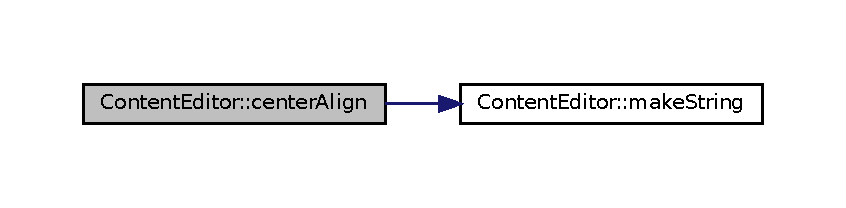
\includegraphics[width=350pt]{class_content_editor_a3c74a024b03eed69ea69ea93d613ffae_cgraph}
\end{center}
\end{figure}
Граф вызова функции\+:\nopagebreak
\begin{figure}[H]
\begin{center}
\leavevmode
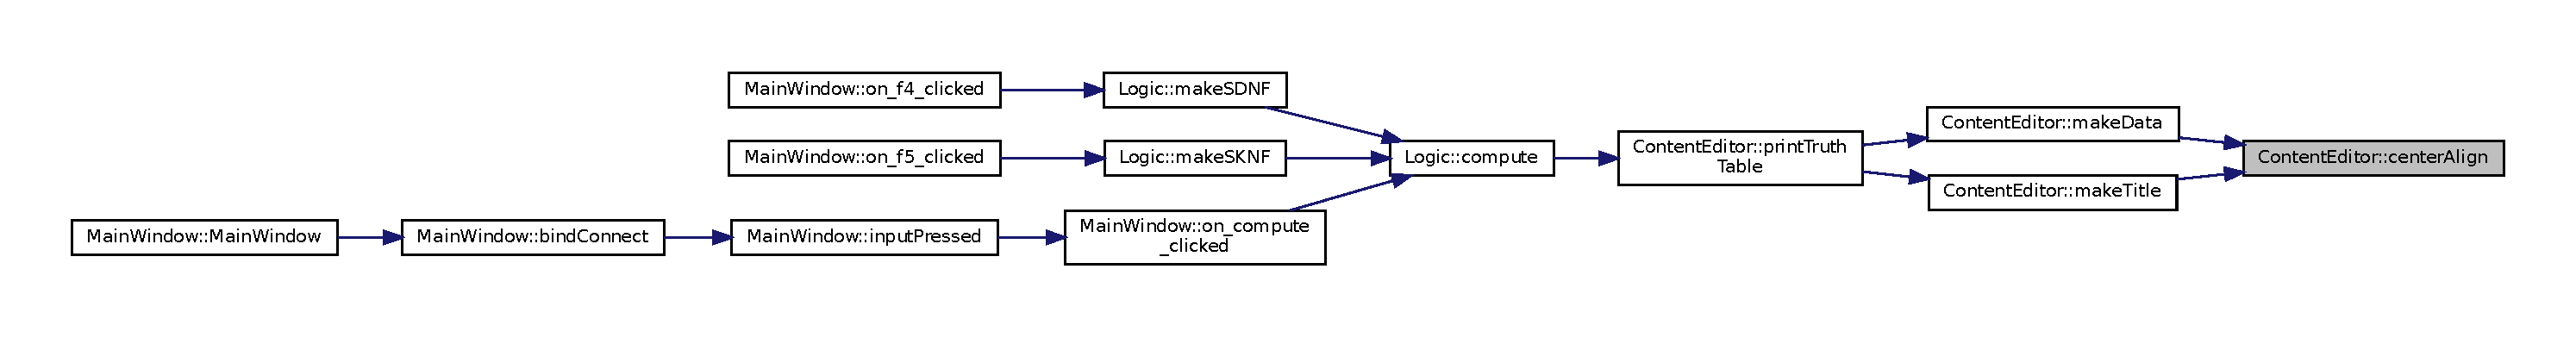
\includegraphics[width=350pt]{class_content_editor_a3c74a024b03eed69ea69ea93d613ffae_icgraph}
\end{center}
\end{figure}
\mbox{\Hypertarget{class_content_editor_a1d600c6051de4c86fd1d3cca6d90a08b}\label{class_content_editor_a1d600c6051de4c86fd1d3cca6d90a08b}} 
\index{ContentEditor@{ContentEditor}!getSize@{getSize}}
\index{getSize@{getSize}!ContentEditor@{ContentEditor}}
\doxysubsubsection{\texorpdfstring{getSize()}{getSize()}}
{\footnotesize\ttfamily Q\+List$<$ int $>$ Content\+Editor\+::get\+Size (\begin{DoxyParamCaption}\item[{const Q\+List$<$ Q\+String $>$ \&}]{title }\end{DoxyParamCaption}) const\hspace{0.3cm}{\ttfamily [private]}}



Размеры ячеек в таблице истинности 

\mbox{\hyperlink{class_content_editor_a1d600c6051de4c86fd1d3cca6d90a08b}{Content\+Editor\+::get\+Size}} Заполняет значения размеров ячеек в таблице истинности cell\+Size\+\_\+.


\begin{DoxyParams}{Аргументы}
{\em title} & список заголовков \\
\hline
\end{DoxyParams}
\begin{DoxyReturn}{Возвращает}
размер, необходимый для каждого из столбцов 
\end{DoxyReturn}
Граф вызова функции\+:\nopagebreak
\begin{figure}[H]
\begin{center}
\leavevmode
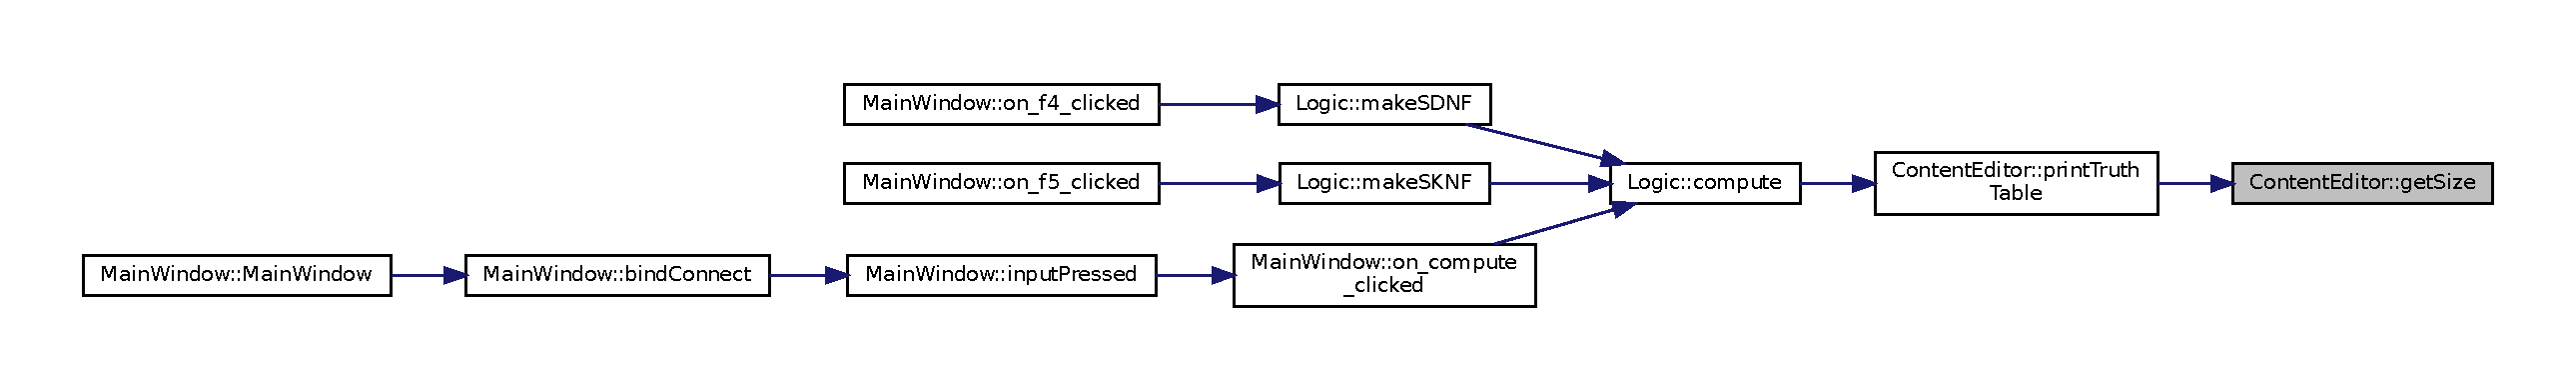
\includegraphics[width=350pt]{class_content_editor_a1d600c6051de4c86fd1d3cca6d90a08b_icgraph}
\end{center}
\end{figure}
\mbox{\Hypertarget{class_content_editor_af0706d1c1595a8417f3a241f7719ab0a}\label{class_content_editor_af0706d1c1595a8417f3a241f7719ab0a}} 
\index{ContentEditor@{ContentEditor}!makeData@{makeData}}
\index{makeData@{makeData}!ContentEditor@{ContentEditor}}
\doxysubsubsection{\texorpdfstring{makeData()}{makeData()}}
{\footnotesize\ttfamily Q\+String Content\+Editor\+::make\+Data (\begin{DoxyParamCaption}\item[{const Q\+List$<$ Q\+List$<$ bool $>$ $>$ \&}]{data }\end{DoxyParamCaption}) const\hspace{0.3cm}{\ttfamily [private]}}



\mbox{\hyperlink{class_content_editor_af0706d1c1595a8417f3a241f7719ab0a}{Content\+Editor\+::make\+Data}} Создает двумерный массив данных $<$0/1$>$ 


\begin{DoxyParams}{Аргументы}
{\em data} & данные, которые необходимо вывести \\
\hline
\end{DoxyParams}
\begin{DoxyReturn}{Возвращает}
итоговая строка с данными 
\end{DoxyReturn}
Граф вызовов\+:\nopagebreak
\begin{figure}[H]
\begin{center}
\leavevmode
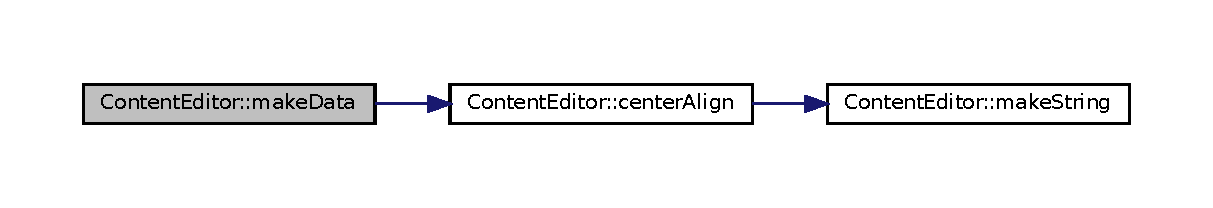
\includegraphics[width=350pt]{class_content_editor_af0706d1c1595a8417f3a241f7719ab0a_cgraph}
\end{center}
\end{figure}
Граф вызова функции\+:\nopagebreak
\begin{figure}[H]
\begin{center}
\leavevmode
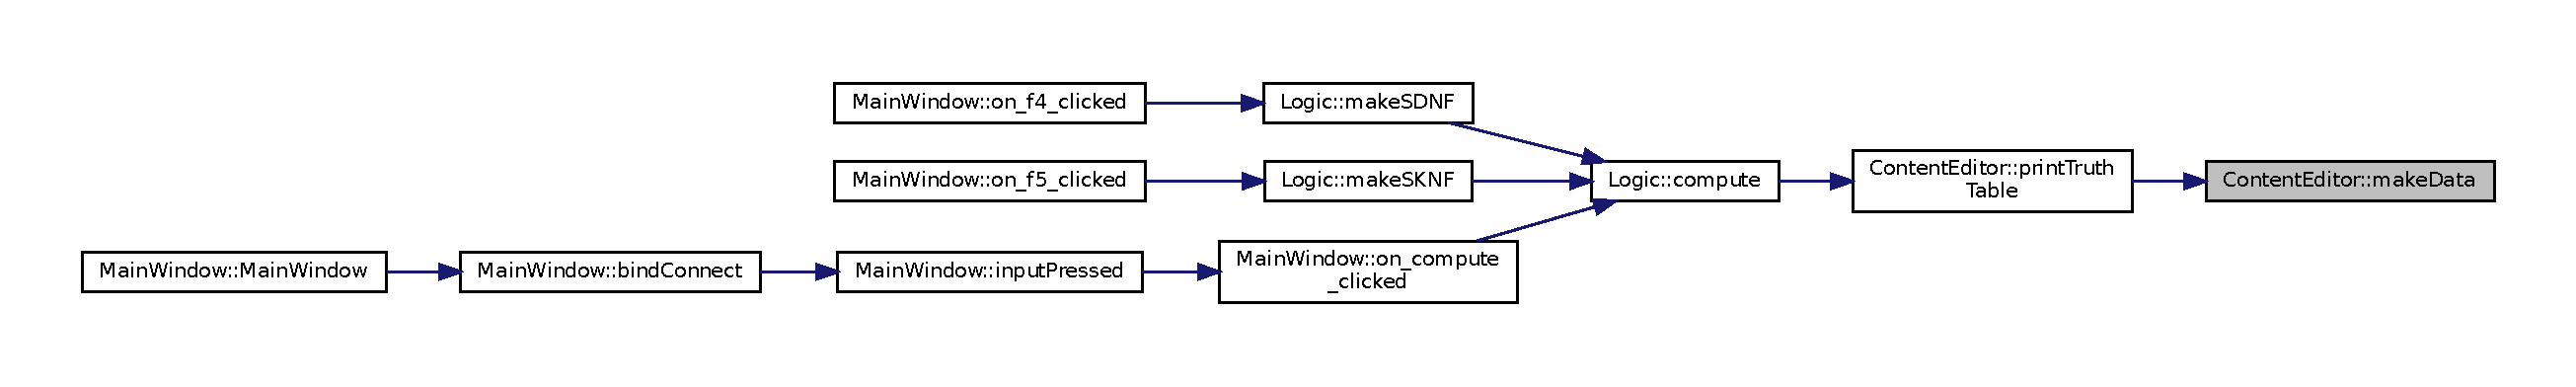
\includegraphics[width=350pt]{class_content_editor_af0706d1c1595a8417f3a241f7719ab0a_icgraph}
\end{center}
\end{figure}
\mbox{\Hypertarget{class_content_editor_a3566d3baaece3ffdf36372ac20301e68}\label{class_content_editor_a3566d3baaece3ffdf36372ac20301e68}} 
\index{ContentEditor@{ContentEditor}!makeLine@{makeLine}}
\index{makeLine@{makeLine}!ContentEditor@{ContentEditor}}
\doxysubsubsection{\texorpdfstring{makeLine()}{makeLine()}}
{\footnotesize\ttfamily Q\+String Content\+Editor\+::make\+Line (\begin{DoxyParamCaption}{ }\end{DoxyParamCaption}) const\hspace{0.3cm}{\ttfamily [private]}}



\mbox{\hyperlink{class_content_editor_a3566d3baaece3ffdf36372ac20301e68}{Content\+Editor\+::make\+Line}} Создает линию под заголовком 

\begin{DoxyReturn}{Возвращает}
получившаяся линия 
\end{DoxyReturn}
Граф вызовов\+:\nopagebreak
\begin{figure}[H]
\begin{center}
\leavevmode
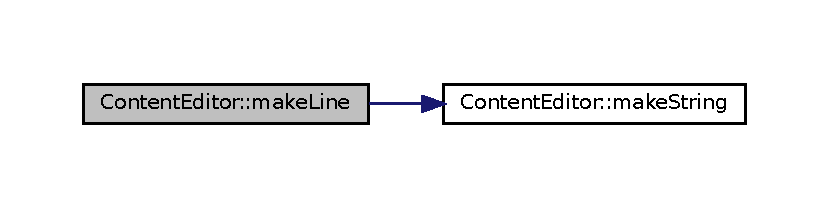
\includegraphics[width=350pt]{class_content_editor_a3566d3baaece3ffdf36372ac20301e68_cgraph}
\end{center}
\end{figure}
Граф вызова функции\+:\nopagebreak
\begin{figure}[H]
\begin{center}
\leavevmode
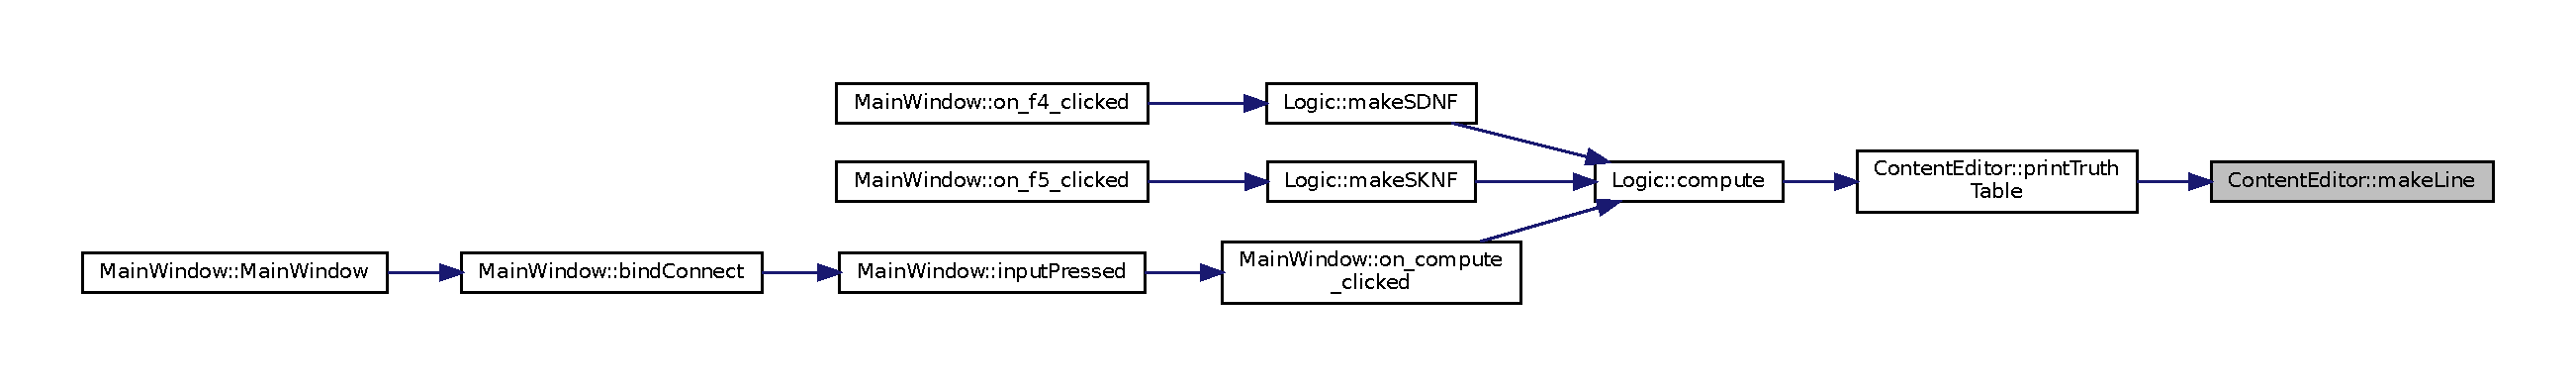
\includegraphics[width=350pt]{class_content_editor_a3566d3baaece3ffdf36372ac20301e68_icgraph}
\end{center}
\end{figure}
\mbox{\Hypertarget{class_content_editor_ab5380863084f8631762f7bb02b7feb72}\label{class_content_editor_ab5380863084f8631762f7bb02b7feb72}} 
\index{ContentEditor@{ContentEditor}!makeString@{makeString}}
\index{makeString@{makeString}!ContentEditor@{ContentEditor}}
\doxysubsubsection{\texorpdfstring{makeString()}{makeString()}}
{\footnotesize\ttfamily Q\+String Content\+Editor\+::make\+String (\begin{DoxyParamCaption}\item[{char}]{segment,  }\item[{int}]{amount }\end{DoxyParamCaption}) const\hspace{0.3cm}{\ttfamily [private]}}



\mbox{\hyperlink{class_content_editor_ab5380863084f8631762f7bb02b7feb72}{Content\+Editor\+::make\+String}} Создает строку из повторяющихся amount раз символов segment. 


\begin{DoxyParams}{Аргументы}
{\em segment} & повторяющийся символ \\
\hline
{\em amount} & сколько раз повторять символ \\
\hline
\end{DoxyParams}
\begin{DoxyReturn}{Возвращает}
получившаяся строка 
\end{DoxyReturn}
Граф вызова функции\+:\nopagebreak
\begin{figure}[H]
\begin{center}
\leavevmode
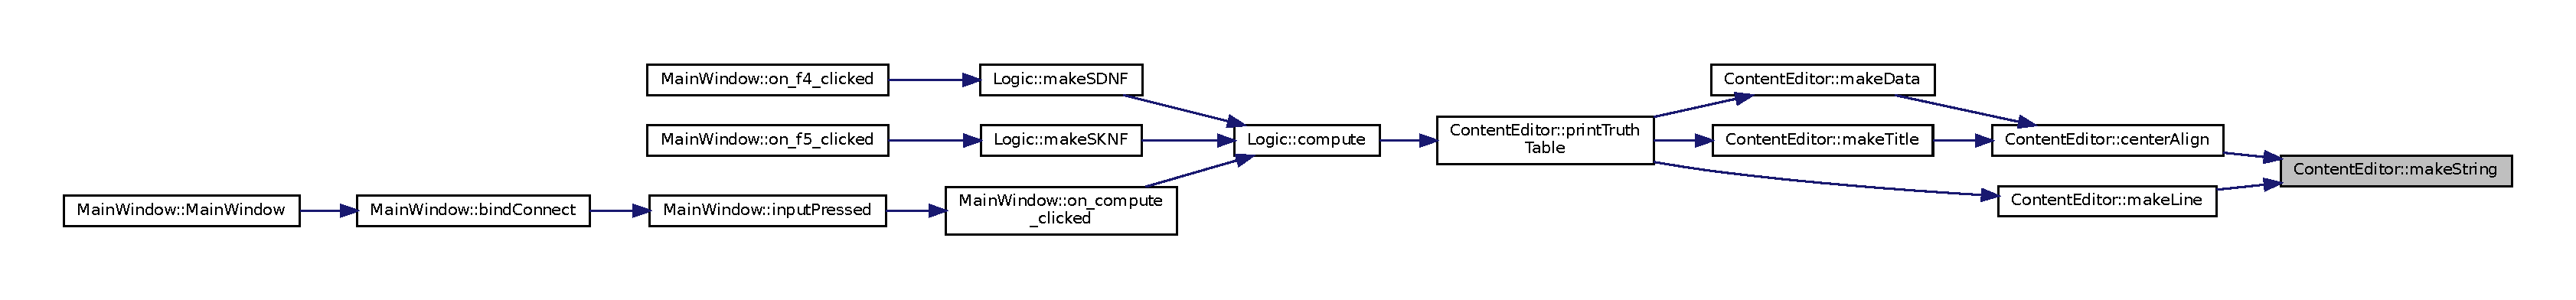
\includegraphics[width=350pt]{class_content_editor_ab5380863084f8631762f7bb02b7feb72_icgraph}
\end{center}
\end{figure}
\mbox{\Hypertarget{class_content_editor_af3c82ca694be2af589491fd361a6b7aa}\label{class_content_editor_af3c82ca694be2af589491fd361a6b7aa}} 
\index{ContentEditor@{ContentEditor}!makeTitle@{makeTitle}}
\index{makeTitle@{makeTitle}!ContentEditor@{ContentEditor}}
\doxysubsubsection{\texorpdfstring{makeTitle()}{makeTitle()}}
{\footnotesize\ttfamily Q\+String Content\+Editor\+::make\+Title (\begin{DoxyParamCaption}\item[{const Q\+List$<$ Q\+String $>$ \&}]{title }\end{DoxyParamCaption}) const\hspace{0.3cm}{\ttfamily [private]}}



\mbox{\hyperlink{class_content_editor_af3c82ca694be2af589491fd361a6b7aa}{Content\+Editor\+::make\+Title}} Создает заголовок 


\begin{DoxyParams}{Аргументы}
{\em title} & текст, который нужно вставить в каждую из колонок заголовка \\
\hline
\end{DoxyParams}
\begin{DoxyReturn}{Возвращает}
получившаяся строка 
\end{DoxyReturn}
Граф вызовов\+:\nopagebreak
\begin{figure}[H]
\begin{center}
\leavevmode
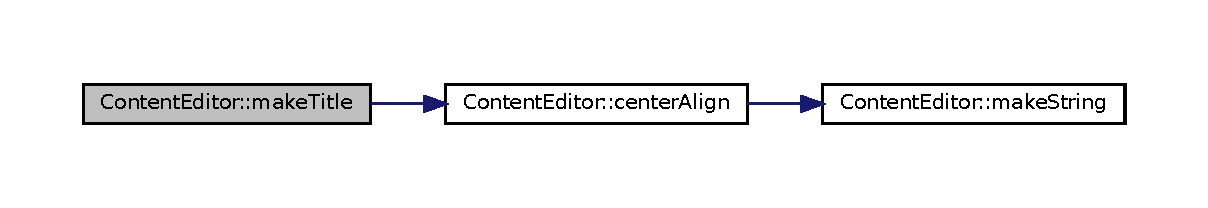
\includegraphics[width=350pt]{class_content_editor_af3c82ca694be2af589491fd361a6b7aa_cgraph}
\end{center}
\end{figure}
Граф вызова функции\+:\nopagebreak
\begin{figure}[H]
\begin{center}
\leavevmode
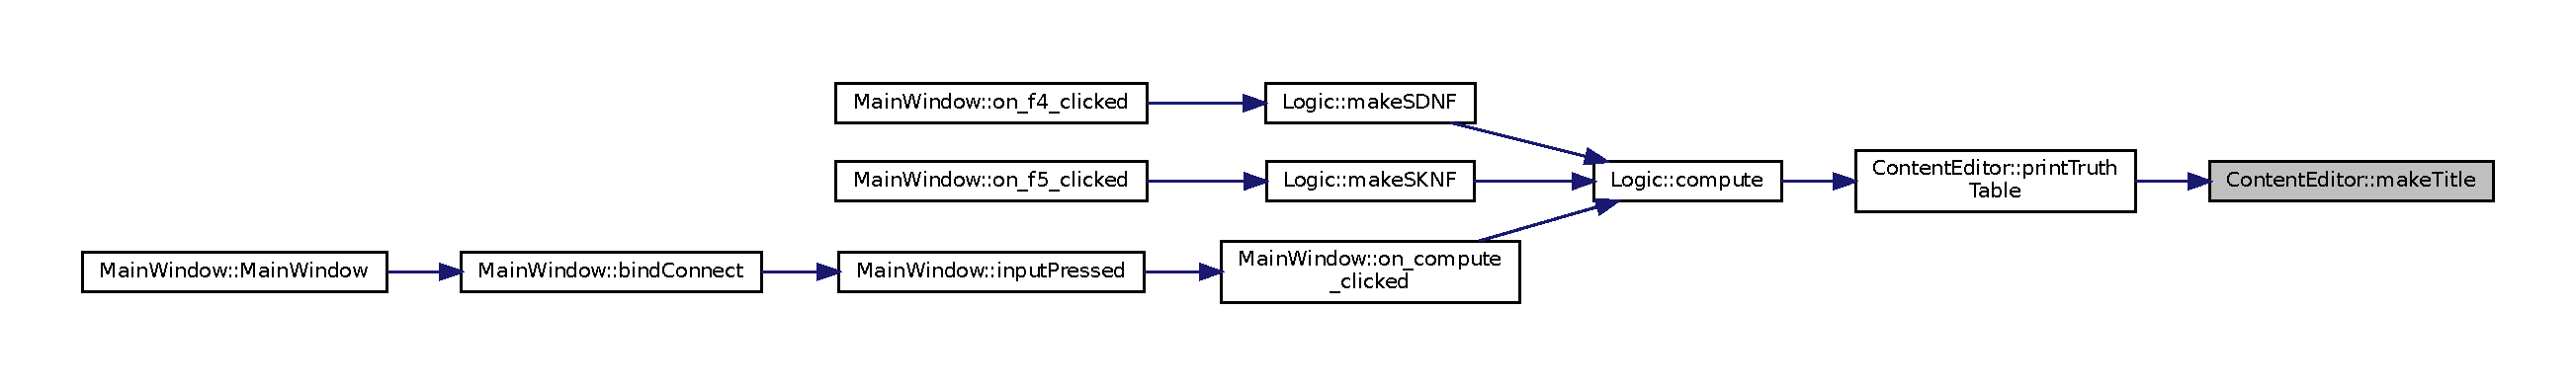
\includegraphics[width=350pt]{class_content_editor_af3c82ca694be2af589491fd361a6b7aa_icgraph}
\end{center}
\end{figure}
\mbox{\Hypertarget{class_content_editor_a929362122ef024a5b4ddc180f8af3423}\label{class_content_editor_a929362122ef024a5b4ddc180f8af3423}} 
\index{ContentEditor@{ContentEditor}!printSDNF@{printSDNF}}
\index{printSDNF@{printSDNF}!ContentEditor@{ContentEditor}}
\doxysubsubsection{\texorpdfstring{printSDNF()}{printSDNF()}}
{\footnotesize\ttfamily void Content\+Editor\+::print\+S\+D\+NF (\begin{DoxyParamCaption}\item[{const Q\+String \&}]{sdnf }\end{DoxyParamCaption}) const}



\mbox{\hyperlink{class_content_editor_a929362122ef024a5b4ddc180f8af3423}{Content\+Editor\+::print\+S\+D\+NF}} выводит Совершенную Дизъюнктивную Нормальную Форму 


\begin{DoxyParams}{Аргументы}
{\em sdnf} & Строка СДНФ \\
\hline
\end{DoxyParams}
Граф вызова функции\+:\nopagebreak
\begin{figure}[H]
\begin{center}
\leavevmode
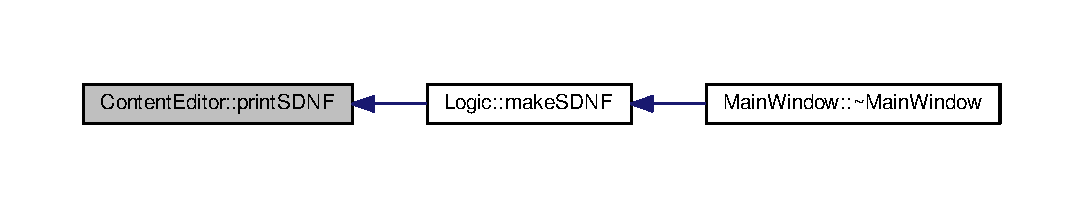
\includegraphics[width=350pt]{class_content_editor_a929362122ef024a5b4ddc180f8af3423_icgraph}
\end{center}
\end{figure}
\mbox{\Hypertarget{class_content_editor_a5492b3c4a67484e9b01322fd6b82870a}\label{class_content_editor_a5492b3c4a67484e9b01322fd6b82870a}} 
\index{ContentEditor@{ContentEditor}!printSKNF@{printSKNF}}
\index{printSKNF@{printSKNF}!ContentEditor@{ContentEditor}}
\doxysubsubsection{\texorpdfstring{printSKNF()}{printSKNF()}}
{\footnotesize\ttfamily void Content\+Editor\+::print\+S\+K\+NF (\begin{DoxyParamCaption}\item[{const Q\+String \&}]{sknf }\end{DoxyParamCaption}) const}



\mbox{\hyperlink{class_content_editor_a5492b3c4a67484e9b01322fd6b82870a}{Content\+Editor\+::print\+S\+K\+NF}} выводит Совершенную Конъюнктивную Нормальную Форму 


\begin{DoxyParams}{Аргументы}
{\em sknf} & Строка СКНФ \\
\hline
\end{DoxyParams}
Граф вызова функции\+:\nopagebreak
\begin{figure}[H]
\begin{center}
\leavevmode
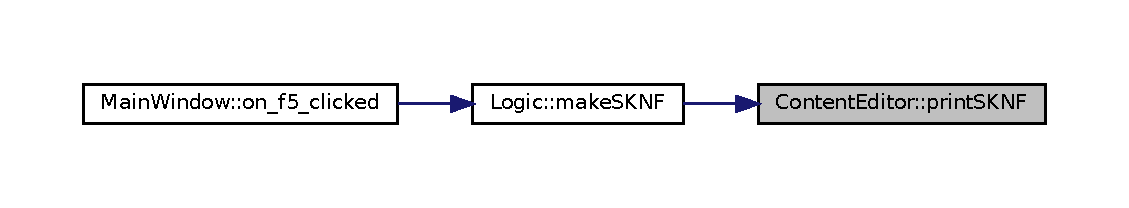
\includegraphics[width=350pt]{class_content_editor_a5492b3c4a67484e9b01322fd6b82870a_icgraph}
\end{center}
\end{figure}
\mbox{\Hypertarget{class_content_editor_a4244e9ccd627ab8146d74637837872e9}\label{class_content_editor_a4244e9ccd627ab8146d74637837872e9}} 
\index{ContentEditor@{ContentEditor}!printTruthTable@{printTruthTable}}
\index{printTruthTable@{printTruthTable}!ContentEditor@{ContentEditor}}
\doxysubsubsection{\texorpdfstring{printTruthTable()}{printTruthTable()}}
{\footnotesize\ttfamily void Content\+Editor\+::print\+Truth\+Table (\begin{DoxyParamCaption}\item[{const Q\+List$<$ Q\+String $>$ \&}]{title,  }\item[{const Q\+List$<$ Q\+List$<$ bool $>$$>$ \&}]{data }\end{DoxyParamCaption})}



\mbox{\hyperlink{class_content_editor_a4244e9ccd627ab8146d74637837872e9}{Content\+Editor\+::print\+Truth\+Table}} Инициирует вывод таблицы истинности 


\begin{DoxyParams}{Аргументы}
{\em title} & заголовок таблицы истинности \\
\hline
{\em data} & данные таблицы истинности \\
\hline
\end{DoxyParams}
Граф вызовов\+:\nopagebreak
\begin{figure}[H]
\begin{center}
\leavevmode
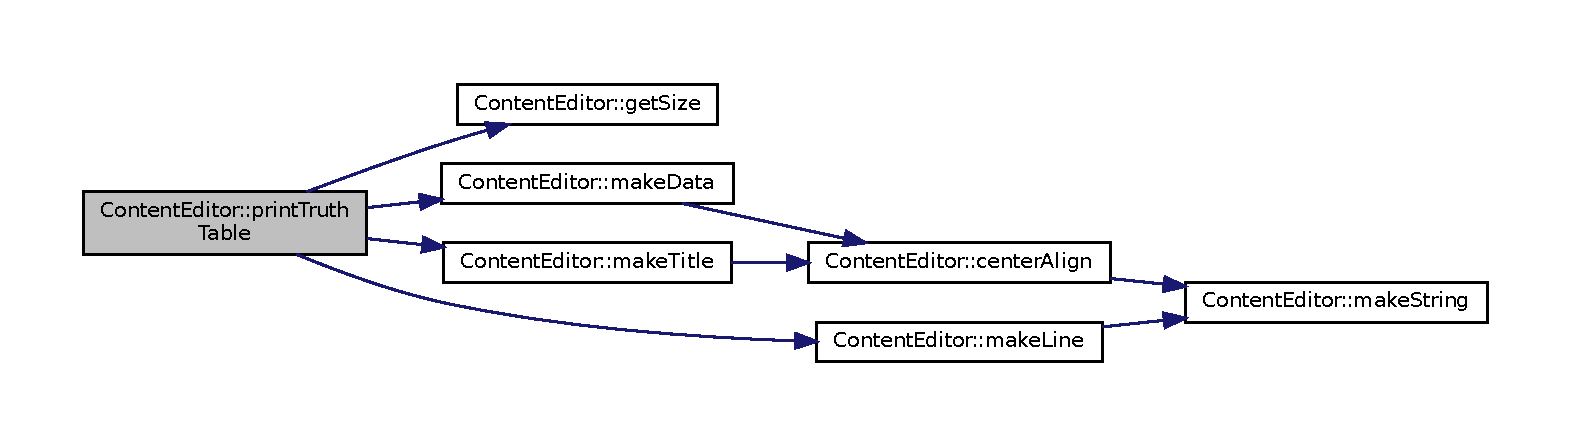
\includegraphics[width=350pt]{class_content_editor_a4244e9ccd627ab8146d74637837872e9_cgraph}
\end{center}
\end{figure}
Граф вызова функции\+:\nopagebreak
\begin{figure}[H]
\begin{center}
\leavevmode
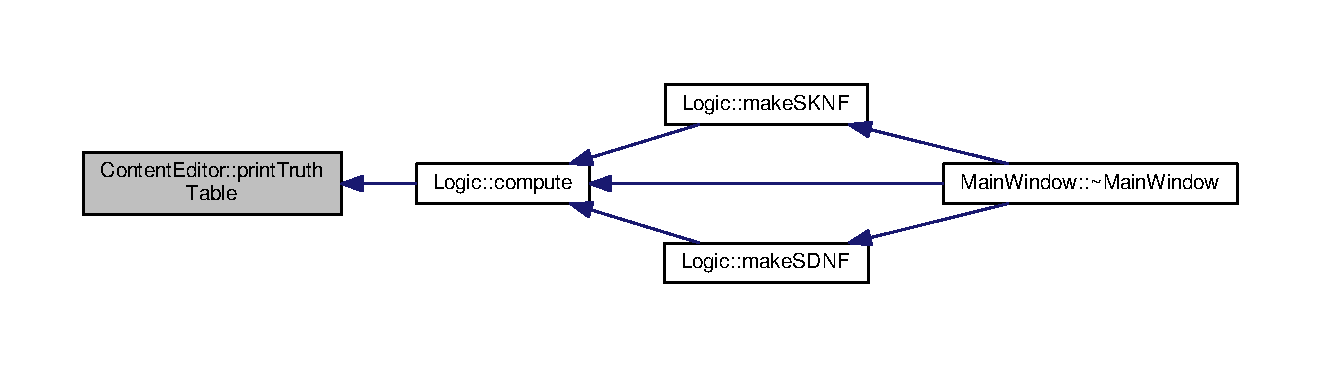
\includegraphics[width=350pt]{class_content_editor_a4244e9ccd627ab8146d74637837872e9_icgraph}
\end{center}
\end{figure}


\doxysubsection{Данные класса}
\mbox{\Hypertarget{class_content_editor_a6bc46e8a608220177a4fbcdee1a50ab9}\label{class_content_editor_a6bc46e8a608220177a4fbcdee1a50ab9}} 
\index{ContentEditor@{ContentEditor}!cellSize\_@{cellSize\_}}
\index{cellSize\_@{cellSize\_}!ContentEditor@{ContentEditor}}
\doxysubsubsection{\texorpdfstring{cellSize\_}{cellSize\_}}
{\footnotesize\ttfamily Q\+List$<$int$>$ Content\+Editor\+::cell\+Size\+\_\+\hspace{0.3cm}{\ttfamily [private]}}



Управление полем вывода 

\mbox{\Hypertarget{class_content_editor_a20a8d18e264777aee600ee638f08eb99}\label{class_content_editor_a20a8d18e264777aee600ee638f08eb99}} 
\index{ContentEditor@{ContentEditor}!minimumColumnCharSize@{minimumColumnCharSize}}
\index{minimumColumnCharSize@{minimumColumnCharSize}!ContentEditor@{ContentEditor}}
\doxysubsubsection{\texorpdfstring{minimumColumnCharSize}{minimumColumnCharSize}}
{\footnotesize\ttfamily const int Content\+Editor\+::minimum\+Column\+Char\+Size = 5}

\mbox{\Hypertarget{class_content_editor_a782c55c84a82d8bd2a11b043995ada2b}\label{class_content_editor_a782c55c84a82d8bd2a11b043995ada2b}} 
\index{ContentEditor@{ContentEditor}!pte\_@{pte\_}}
\index{pte\_@{pte\_}!ContentEditor@{ContentEditor}}
\doxysubsubsection{\texorpdfstring{pte\_}{pte\_}}
{\footnotesize\ttfamily Q\+Plain\+Text\+Edit$\ast$ Content\+Editor\+::pte\+\_\+\hspace{0.3cm}{\ttfamily [private]}}



Минимальный размер столбца в символах 



Объявления и описания членов классов находятся в файлах\+:\begin{DoxyCompactItemize}
\item 
/home/mike/projects/logic\+\_\+calculator/\mbox{\hyperlink{contenteditor_8h}{contenteditor.\+h}}\item 
/home/mike/projects/logic\+\_\+calculator/\mbox{\hyperlink{contenteditor_8cpp}{contenteditor.\+cpp}}\end{DoxyCompactItemize}

\hypertarget{class_input_editor}{}\doxysection{Класс Input\+Editor}
\label{class_input_editor}\index{InputEditor@{InputEditor}}


\mbox{\hyperlink{class_input_editor}{Input\+Editor}} -\/ Класс отвечает за обработку данных, вводимых в поле ввода данных  




{\ttfamily \#include $<$inputeditor.\+h$>$}

\doxysubsection*{Открытые члены}
\begin{DoxyCompactItemize}
\item 
\mbox{\hyperlink{class_input_editor_ac9aae2a915a58eae586aa373c1b1f635}{Input\+Editor}} (Q\+Line\+Edit $\ast$input)
\item 
\mbox{\hyperlink{class_input_editor_aec1a586153ea14380867eff2c7605bec}{$\sim$\+Input\+Editor}} ()
\item 
void \mbox{\hyperlink{class_input_editor_a4b357e281c2d9cf669ed4a03c8de5190}{push\+Back}} (const Q\+String \&str)
\begin{DoxyCompactList}\small\item\em словарь доступных действий \end{DoxyCompactList}\item 
Q\+String \mbox{\hyperlink{class_input_editor_ab65dc1f4a87be3abf8bfff14c1a54532}{to\+String}} () const
\begin{DoxyCompactList}\small\item\em \mbox{\hyperlink{class_input_editor_ab65dc1f4a87be3abf8bfff14c1a54532}{Input\+Editor\+::to\+String}} Преобразует внутренний массив в строку \end{DoxyCompactList}\item 
bool \mbox{\hyperlink{class_input_editor_ad9a9e03d439e909c6d72775ef78d9814}{parse}} (const Q\+String \&str)
\begin{DoxyCompactList}\small\item\em \mbox{\hyperlink{class_input_editor_ad9a9e03d439e909c6d72775ef78d9814}{Input\+Editor\+::parse}} Парсит введенную строку \end{DoxyCompactList}\item 
Q\+List$<$ Q\+String $>$ $\ast$ \mbox{\hyperlink{class_input_editor_a3f69e5b7fe43e31f2a4f783fbdc8072e}{get\+Vars}} ()
\begin{DoxyCompactList}\small\item\em \mbox{\hyperlink{class_input_editor_a3f69e5b7fe43e31f2a4f783fbdc8072e}{Input\+Editor\+::get\+Vars}} Выдает указатель на внутренний массив данных \end{DoxyCompactList}\end{DoxyCompactItemize}
\doxysubsection*{Открытые атрибуты}
\begin{DoxyCompactItemize}
\item 
const Q\+List$<$ Q\+String $>$ \mbox{\hyperlink{class_input_editor_a2c1e4bffaceced12c4f13e3f19a80fb7}{A\+V\+I\+A\+B\+L\+E\+\_\+\+W\+O\+R\+DS}}
\item 
const Q\+Map$<$ Q\+String, Q\+String $>$ \mbox{\hyperlink{class_input_editor_a328642e3ae078e059dc95bb4f945451c}{A\+V\+I\+A\+B\+L\+E\+\_\+\+T\+R\+A\+N\+S\+F\+O\+R\+M\+A\+T\+I\+O\+NS}}
\begin{DoxyCompactList}\small\item\em Словарь доступных символов \end{DoxyCompactList}\end{DoxyCompactItemize}
\doxysubsection*{Закрытые члены}
\begin{DoxyCompactItemize}
\item 
void \mbox{\hyperlink{class_input_editor_a592b851c7b18ab7f0cbfcf64bdff3d9d}{update\+Input}} ()
\begin{DoxyCompactList}\small\item\em Внутренний массив для хранения данных из поля ввода данных \end{DoxyCompactList}\item 
bool \mbox{\hyperlink{class_input_editor_a6e53e6455f8a3948620a61e68a089520}{is\+Validity}} () const
\item 
Q\+String \mbox{\hyperlink{class_input_editor_a86f05f35fe5a16552cfd545d106d2585}{normalize\+String}} (const Q\+String \&input) const
\end{DoxyCompactItemize}
\doxysubsection*{Закрытые данные}
\begin{DoxyCompactItemize}
\item 
Q\+Line\+Edit $\ast$ \mbox{\hyperlink{class_input_editor_abd7448dec9d9badf5a80fb78d8a4ca9b}{input\+\_\+}}
\item 
Q\+List$<$ Q\+String $>$ $\ast$ \mbox{\hyperlink{class_input_editor_a8ededb30c2f014d27f5432ea29b6da92}{v\+\_\+}}
\begin{DoxyCompactList}\small\item\em Используется для управления полем ввода данных \end{DoxyCompactList}\end{DoxyCompactItemize}


\doxysubsection{Подробное описание}
\mbox{\hyperlink{class_input_editor}{Input\+Editor}} -\/ Класс отвечает за обработку данных, вводимых в поле ввода данных 

\doxysubsection{Конструктор(ы)}
\mbox{\Hypertarget{class_input_editor_ac9aae2a915a58eae586aa373c1b1f635}\label{class_input_editor_ac9aae2a915a58eae586aa373c1b1f635}} 
\index{InputEditor@{InputEditor}!InputEditor@{InputEditor}}
\index{InputEditor@{InputEditor}!InputEditor@{InputEditor}}
\doxysubsubsection{\texorpdfstring{InputEditor()}{InputEditor()}}
{\footnotesize\ttfamily Input\+Editor\+::\+Input\+Editor (\begin{DoxyParamCaption}\item[{Q\+Line\+Edit $\ast$}]{input }\end{DoxyParamCaption})}

\begin{Desc}
\item[Примеры]\par
\mbox{\hyperlink{_2home_2mike_2projects_2logic_calculator_2inputeditor_8cpp-example}{/home/mike/projects/logic\+\_\+calculator/inputeditor.\+cpp}}.\end{Desc}
\mbox{\Hypertarget{class_input_editor_aec1a586153ea14380867eff2c7605bec}\label{class_input_editor_aec1a586153ea14380867eff2c7605bec}} 
\index{InputEditor@{InputEditor}!````~InputEditor@{$\sim$InputEditor}}
\index{````~InputEditor@{$\sim$InputEditor}!InputEditor@{InputEditor}}
\doxysubsubsection{\texorpdfstring{$\sim$InputEditor()}{~InputEditor()}}
{\footnotesize\ttfamily Input\+Editor\+::$\sim$\+Input\+Editor (\begin{DoxyParamCaption}{ }\end{DoxyParamCaption})}

\begin{Desc}
\item[Примеры]\par
\mbox{\hyperlink{_2home_2mike_2projects_2logic_calculator_2inputeditor_8cpp-example}{/home/mike/projects/logic\+\_\+calculator/inputeditor.\+cpp}}.\end{Desc}


\doxysubsection{Методы}
\mbox{\Hypertarget{class_input_editor_a3f69e5b7fe43e31f2a4f783fbdc8072e}\label{class_input_editor_a3f69e5b7fe43e31f2a4f783fbdc8072e}} 
\index{InputEditor@{InputEditor}!getVars@{getVars}}
\index{getVars@{getVars}!InputEditor@{InputEditor}}
\doxysubsubsection{\texorpdfstring{getVars()}{getVars()}}
{\footnotesize\ttfamily Q\+List$<$ Q\+String $>$ $\ast$ Input\+Editor\+::get\+Vars (\begin{DoxyParamCaption}{ }\end{DoxyParamCaption})}



\mbox{\hyperlink{class_input_editor_a3f69e5b7fe43e31f2a4f783fbdc8072e}{Input\+Editor\+::get\+Vars}} Выдает указатель на внутренний массив данных 

\begin{DoxyReturn}{Возвращает}
Указатель на внутренний массив данных 
\end{DoxyReturn}
\begin{Desc}
\item[Примеры]\par
\mbox{\hyperlink{_2home_2mike_2projects_2logic_calculator_2inputeditor_8cpp-example}{/home/mike/projects/logic\+\_\+calculator/inputeditor.\+cpp}}.\end{Desc}
Граф вызова функции\+:\nopagebreak
\begin{figure}[H]
\begin{center}
\leavevmode
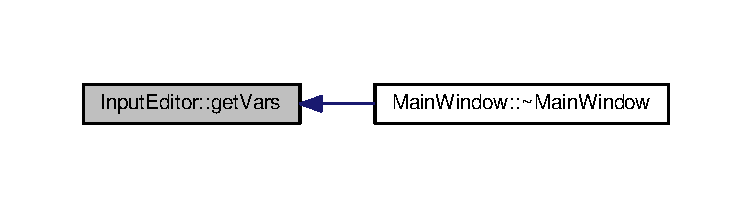
\includegraphics[width=350pt]{class_input_editor_a3f69e5b7fe43e31f2a4f783fbdc8072e_icgraph}
\end{center}
\end{figure}
\mbox{\Hypertarget{class_input_editor_a6e53e6455f8a3948620a61e68a089520}\label{class_input_editor_a6e53e6455f8a3948620a61e68a089520}} 
\index{InputEditor@{InputEditor}!isValidity@{isValidity}}
\index{isValidity@{isValidity}!InputEditor@{InputEditor}}
\doxysubsubsection{\texorpdfstring{isValidity()}{isValidity()}}
{\footnotesize\ttfamily bool Input\+Editor\+::is\+Validity (\begin{DoxyParamCaption}{ }\end{DoxyParamCaption}) const\hspace{0.3cm}{\ttfamily [private]}}

\begin{Desc}
\item[Примеры]\par
\mbox{\hyperlink{_2home_2mike_2projects_2logic_calculator_2inputeditor_8cpp-example}{/home/mike/projects/logic\+\_\+calculator/inputeditor.\+cpp}}.\end{Desc}
Граф вызовов\+:\nopagebreak
\begin{figure}[H]
\begin{center}
\leavevmode
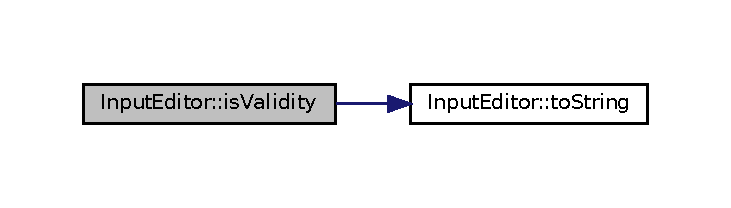
\includegraphics[width=350pt]{class_input_editor_a6e53e6455f8a3948620a61e68a089520_cgraph}
\end{center}
\end{figure}
Граф вызова функции\+:\nopagebreak
\begin{figure}[H]
\begin{center}
\leavevmode
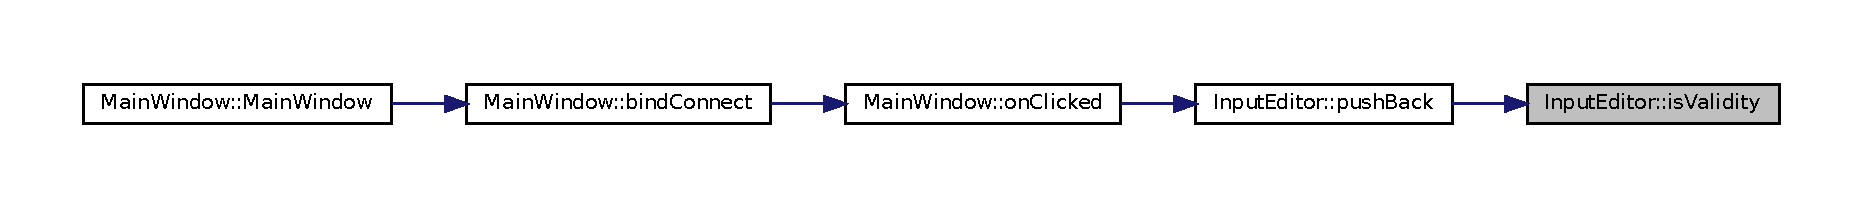
\includegraphics[width=350pt]{class_input_editor_a6e53e6455f8a3948620a61e68a089520_icgraph}
\end{center}
\end{figure}
\mbox{\Hypertarget{class_input_editor_a86f05f35fe5a16552cfd545d106d2585}\label{class_input_editor_a86f05f35fe5a16552cfd545d106d2585}} 
\index{InputEditor@{InputEditor}!normalizeString@{normalizeString}}
\index{normalizeString@{normalizeString}!InputEditor@{InputEditor}}
\doxysubsubsection{\texorpdfstring{normalizeString()}{normalizeString()}}
{\footnotesize\ttfamily Q\+String Input\+Editor\+::normalize\+String (\begin{DoxyParamCaption}\item[{const Q\+String \&}]{input }\end{DoxyParamCaption}) const\hspace{0.3cm}{\ttfamily [private]}}

\begin{Desc}
\item[Примеры]\par
\mbox{\hyperlink{_2home_2mike_2projects_2logic_calculator_2inputeditor_8cpp-example}{/home/mike/projects/logic\+\_\+calculator/inputeditor.\+cpp}}.\end{Desc}
Граф вызова функции\+:\nopagebreak
\begin{figure}[H]
\begin{center}
\leavevmode
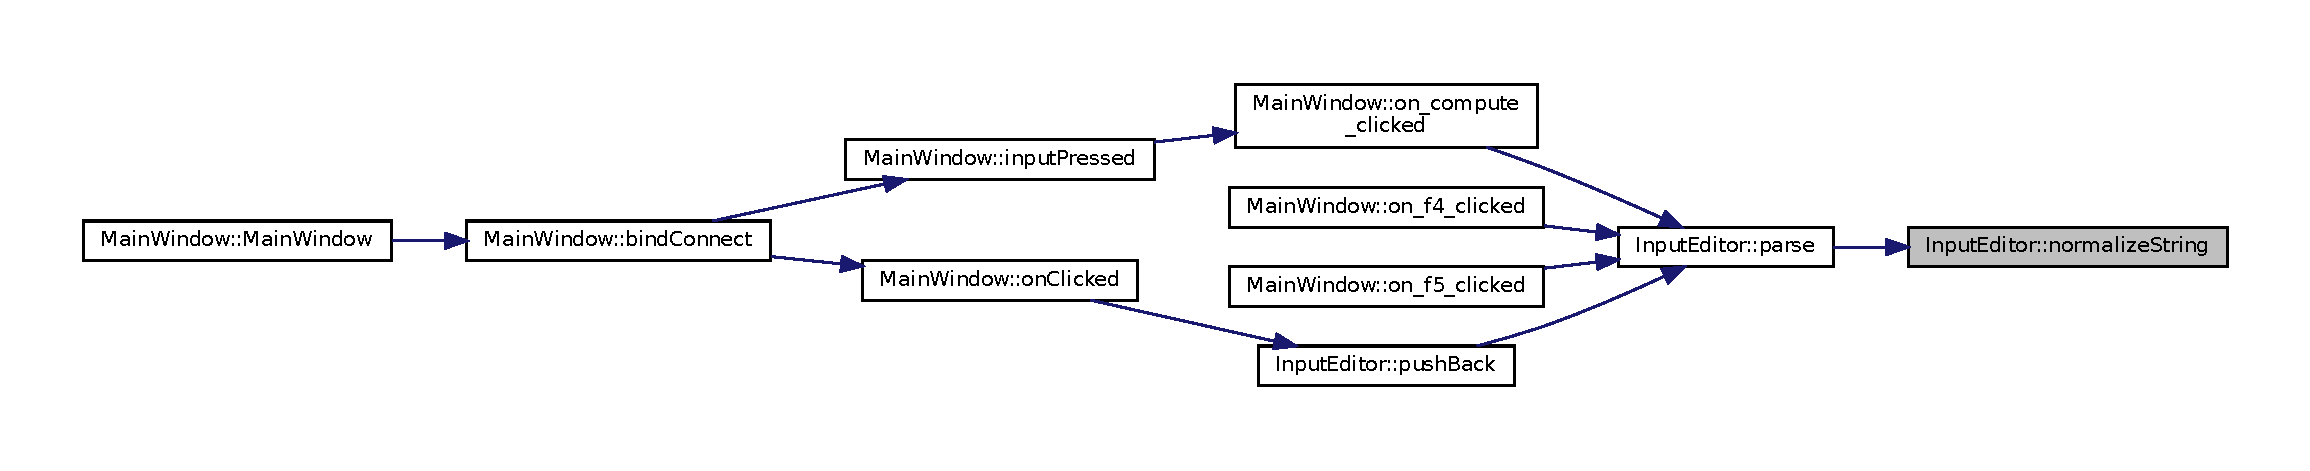
\includegraphics[width=350pt]{class_input_editor_a86f05f35fe5a16552cfd545d106d2585_icgraph}
\end{center}
\end{figure}
\mbox{\Hypertarget{class_input_editor_ad9a9e03d439e909c6d72775ef78d9814}\label{class_input_editor_ad9a9e03d439e909c6d72775ef78d9814}} 
\index{InputEditor@{InputEditor}!parse@{parse}}
\index{parse@{parse}!InputEditor@{InputEditor}}
\doxysubsubsection{\texorpdfstring{parse()}{parse()}}
{\footnotesize\ttfamily bool Input\+Editor\+::parse (\begin{DoxyParamCaption}\item[{const Q\+String \&}]{str }\end{DoxyParamCaption})}



\mbox{\hyperlink{class_input_editor_ad9a9e03d439e909c6d72775ef78d9814}{Input\+Editor\+::parse}} Парсит введенную строку 


\begin{DoxyParams}{Аргументы}
{\em str} & строка для парсинга \\
\hline
\end{DoxyParams}
\begin{DoxyReturn}{Возвращает}
смогло ли произойти чтение 
\end{DoxyReturn}
\begin{Desc}
\item[Примеры]\par
\mbox{\hyperlink{_2home_2mike_2projects_2logic_calculator_2inputeditor_8cpp-example}{/home/mike/projects/logic\+\_\+calculator/inputeditor.\+cpp}}.\end{Desc}
Граф вызовов\+:\nopagebreak
\begin{figure}[H]
\begin{center}
\leavevmode
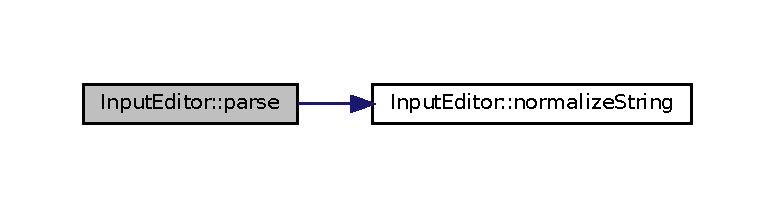
\includegraphics[width=350pt]{class_input_editor_ad9a9e03d439e909c6d72775ef78d9814_cgraph}
\end{center}
\end{figure}
Граф вызова функции\+:\nopagebreak
\begin{figure}[H]
\begin{center}
\leavevmode
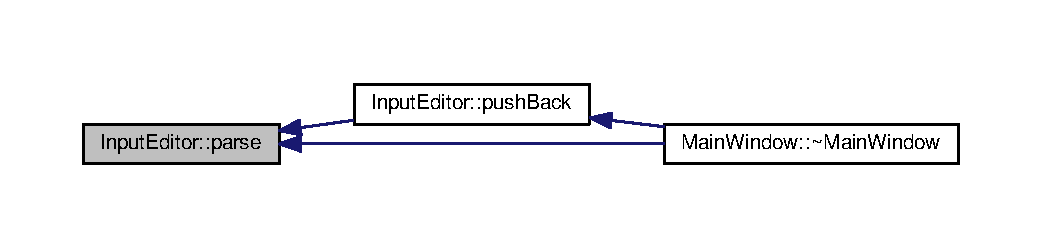
\includegraphics[width=350pt]{class_input_editor_ad9a9e03d439e909c6d72775ef78d9814_icgraph}
\end{center}
\end{figure}
\mbox{\Hypertarget{class_input_editor_a4b357e281c2d9cf669ed4a03c8de5190}\label{class_input_editor_a4b357e281c2d9cf669ed4a03c8de5190}} 
\index{InputEditor@{InputEditor}!pushBack@{pushBack}}
\index{pushBack@{pushBack}!InputEditor@{InputEditor}}
\doxysubsubsection{\texorpdfstring{pushBack()}{pushBack()}}
{\footnotesize\ttfamily void Input\+Editor\+::push\+Back (\begin{DoxyParamCaption}\item[{const Q\+String \&}]{str }\end{DoxyParamCaption})}



словарь доступных действий 

\mbox{\hyperlink{class_input_editor_a4b357e281c2d9cf669ed4a03c8de5190}{Input\+Editor\+::push\+Back}} Добавляет определенные данные в конец внутреннего массива


\begin{DoxyParams}{Аргументы}
{\em str} & данные \\
\hline
\end{DoxyParams}
\begin{Desc}
\item[Примеры]\par
\mbox{\hyperlink{_2home_2mike_2projects_2logic_calculator_2inputeditor_8cpp-example}{/home/mike/projects/logic\+\_\+calculator/inputeditor.\+cpp}}.\end{Desc}
Граф вызовов\+:\nopagebreak
\begin{figure}[H]
\begin{center}
\leavevmode
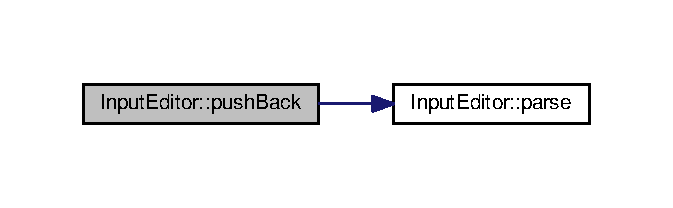
\includegraphics[width=350pt]{class_input_editor_a4b357e281c2d9cf669ed4a03c8de5190_cgraph}
\end{center}
\end{figure}
Граф вызова функции\+:\nopagebreak
\begin{figure}[H]
\begin{center}
\leavevmode
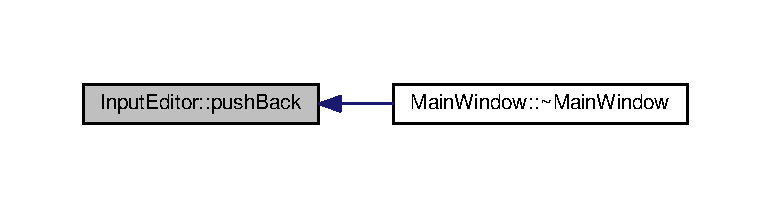
\includegraphics[width=350pt]{class_input_editor_a4b357e281c2d9cf669ed4a03c8de5190_icgraph}
\end{center}
\end{figure}
\mbox{\Hypertarget{class_input_editor_ab65dc1f4a87be3abf8bfff14c1a54532}\label{class_input_editor_ab65dc1f4a87be3abf8bfff14c1a54532}} 
\index{InputEditor@{InputEditor}!toString@{toString}}
\index{toString@{toString}!InputEditor@{InputEditor}}
\doxysubsubsection{\texorpdfstring{toString()}{toString()}}
{\footnotesize\ttfamily Q\+String Input\+Editor\+::to\+String (\begin{DoxyParamCaption}{ }\end{DoxyParamCaption}) const}



\mbox{\hyperlink{class_input_editor_ab65dc1f4a87be3abf8bfff14c1a54532}{Input\+Editor\+::to\+String}} Преобразует внутренний массив в строку 

\begin{DoxyReturn}{Возвращает}
сгенерированная строка 
\end{DoxyReturn}
\begin{Desc}
\item[Примеры]\par
\mbox{\hyperlink{_2home_2mike_2projects_2logic_calculator_2inputeditor_8cpp-example}{/home/mike/projects/logic\+\_\+calculator/inputeditor.\+cpp}}.\end{Desc}
Граф вызова функции\+:\nopagebreak
\begin{figure}[H]
\begin{center}
\leavevmode
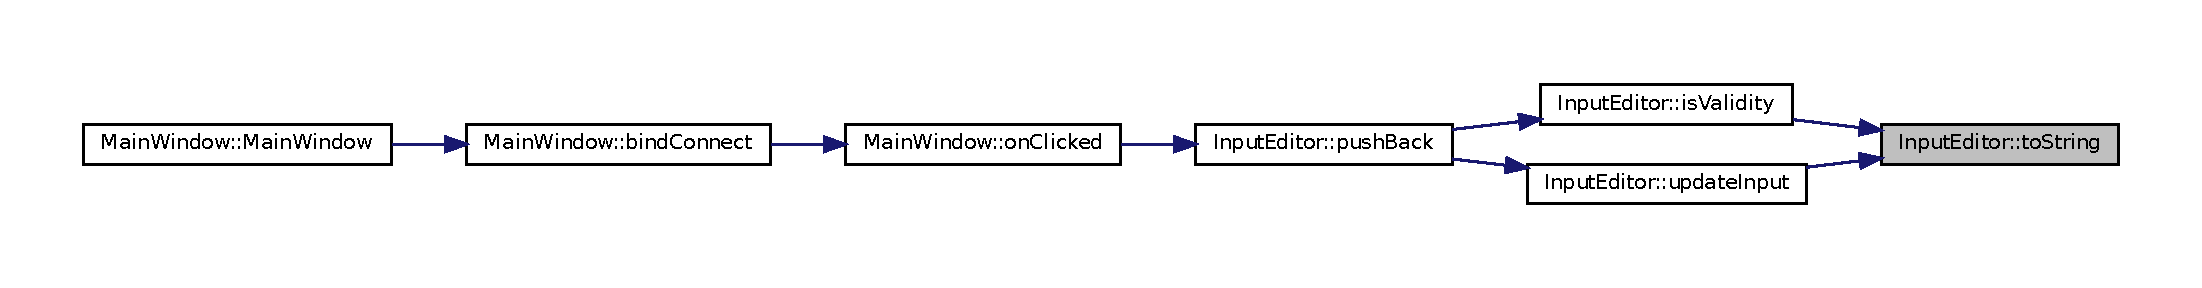
\includegraphics[width=350pt]{class_input_editor_ab65dc1f4a87be3abf8bfff14c1a54532_icgraph}
\end{center}
\end{figure}
\mbox{\Hypertarget{class_input_editor_a592b851c7b18ab7f0cbfcf64bdff3d9d}\label{class_input_editor_a592b851c7b18ab7f0cbfcf64bdff3d9d}} 
\index{InputEditor@{InputEditor}!updateInput@{updateInput}}
\index{updateInput@{updateInput}!InputEditor@{InputEditor}}
\doxysubsubsection{\texorpdfstring{updateInput()}{updateInput()}}
{\footnotesize\ttfamily void Input\+Editor\+::update\+Input (\begin{DoxyParamCaption}{ }\end{DoxyParamCaption})\hspace{0.3cm}{\ttfamily [private]}}



Внутренний массив для хранения данных из поля ввода данных 

\mbox{\hyperlink{class_input_editor_a592b851c7b18ab7f0cbfcf64bdff3d9d}{Input\+Editor\+::update\+Input}} Обновляет поле для ввода данных \begin{Desc}
\item[Примеры]\par
\mbox{\hyperlink{_2home_2mike_2projects_2logic_calculator_2inputeditor_8cpp-example}{/home/mike/projects/logic\+\_\+calculator/inputeditor.\+cpp}}.\end{Desc}
Граф вызовов\+:\nopagebreak
\begin{figure}[H]
\begin{center}
\leavevmode
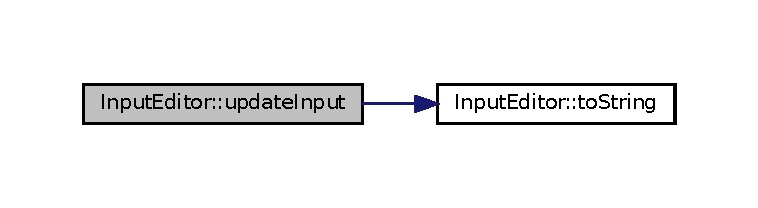
\includegraphics[width=350pt]{class_input_editor_a592b851c7b18ab7f0cbfcf64bdff3d9d_cgraph}
\end{center}
\end{figure}
Граф вызова функции\+:\nopagebreak
\begin{figure}[H]
\begin{center}
\leavevmode
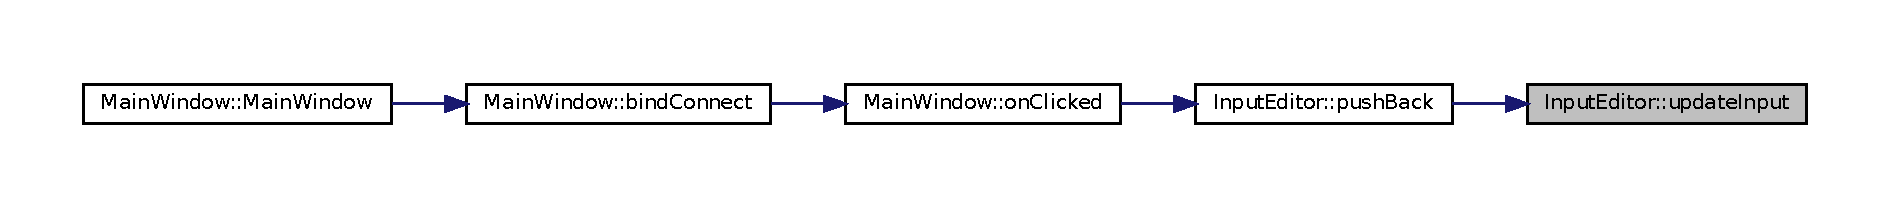
\includegraphics[width=350pt]{class_input_editor_a592b851c7b18ab7f0cbfcf64bdff3d9d_icgraph}
\end{center}
\end{figure}


\doxysubsection{Данные класса}
\mbox{\Hypertarget{class_input_editor_a328642e3ae078e059dc95bb4f945451c}\label{class_input_editor_a328642e3ae078e059dc95bb4f945451c}} 
\index{InputEditor@{InputEditor}!AVIABLE\_TRANSFORMATIONS@{AVIABLE\_TRANSFORMATIONS}}
\index{AVIABLE\_TRANSFORMATIONS@{AVIABLE\_TRANSFORMATIONS}!InputEditor@{InputEditor}}
\doxysubsubsection{\texorpdfstring{AVIABLE\_TRANSFORMATIONS}{AVIABLE\_TRANSFORMATIONS}}
{\footnotesize\ttfamily const Q\+Map$<$Q\+String,Q\+String$>$ Input\+Editor\+::\+A\+V\+I\+A\+B\+L\+E\+\_\+\+T\+R\+A\+N\+S\+F\+O\+R\+M\+A\+T\+I\+O\+NS}

{\bfseries Инициализатор}
\begin{DoxyCode}{0}
\DoxyCodeLine{\{}
\DoxyCodeLine{        \{\textcolor{stringliteral}{"conjunction"}, \textcolor{stringliteral}{"*"}\},}
\DoxyCodeLine{        \{\textcolor{stringliteral}{"disjunction"}, \textcolor{stringliteral}{"+"}\},}
\DoxyCodeLine{        \{\textcolor{stringliteral}{"exclusive\_disjunction"}, \textcolor{stringliteral}{"\string^"}\},}
\DoxyCodeLine{        \{\textcolor{stringliteral}{"not\_and"}, \textcolor{stringliteral}{"|"}\},}
\DoxyCodeLine{        \{\textcolor{stringliteral}{"not\_or"}, \textcolor{stringliteral}{"\#"}\},}
\DoxyCodeLine{        \{\textcolor{stringliteral}{"implication"}, \textcolor{stringliteral}{"-\/>"}\},}
\DoxyCodeLine{        \{\textcolor{stringliteral}{"converse"}, \textcolor{stringliteral}{"<-\/"}\},}
\DoxyCodeLine{        \{\textcolor{stringliteral}{"equivalent"}, \textcolor{stringliteral}{"\string~"}\},}
\DoxyCodeLine{        \{\textcolor{stringliteral}{"negation"}, \textcolor{stringliteral}{"!"}\}}
\DoxyCodeLine{    \}}

\end{DoxyCode}


Словарь доступных символов 

\mbox{\Hypertarget{class_input_editor_a2c1e4bffaceced12c4f13e3f19a80fb7}\label{class_input_editor_a2c1e4bffaceced12c4f13e3f19a80fb7}} 
\index{InputEditor@{InputEditor}!AVIABLE\_WORDS@{AVIABLE\_WORDS}}
\index{AVIABLE\_WORDS@{AVIABLE\_WORDS}!InputEditor@{InputEditor}}
\doxysubsubsection{\texorpdfstring{AVIABLE\_WORDS}{AVIABLE\_WORDS}}
{\footnotesize\ttfamily const Q\+List$<$Q\+String$>$ Input\+Editor\+::\+A\+V\+I\+A\+B\+L\+E\+\_\+\+W\+O\+R\+DS}

{\bfseries Инициализатор}
\begin{DoxyCode}{0}
\DoxyCodeLine{\{}
\DoxyCodeLine{        \textcolor{stringliteral}{"*"} , \textcolor{stringliteral}{"+"} , \textcolor{stringliteral}{"!"} , \textcolor{stringliteral}{"\string^"} , \textcolor{stringliteral}{"-\/>"} , \textcolor{stringliteral}{"<-\/"} , \textcolor{stringliteral}{"\string~"} , \textcolor{stringliteral}{"|"} , \textcolor{stringliteral}{"\#"},}
\DoxyCodeLine{        \textcolor{stringliteral}{"A"} , \textcolor{stringliteral}{"B"} , \textcolor{stringliteral}{"C"} , \textcolor{stringliteral}{"D"} , \textcolor{stringliteral}{"E"} , \textcolor{stringliteral}{"F"} , \textcolor{stringliteral}{"G"} , \textcolor{stringliteral}{"X"} , \textcolor{stringliteral}{"Y"} , \textcolor{stringliteral}{"Z"},}
\DoxyCodeLine{        \textcolor{stringliteral}{"a"} , \textcolor{stringliteral}{"b"} , \textcolor{stringliteral}{"c"} , \textcolor{stringliteral}{"d"} , \textcolor{stringliteral}{"e"} , \textcolor{stringliteral}{"f"} , \textcolor{stringliteral}{"g"} , \textcolor{stringliteral}{"x"} , \textcolor{stringliteral}{"y"} , \textcolor{stringliteral}{"z"},}
\DoxyCodeLine{        \textcolor{stringliteral}{"("} , \textcolor{stringliteral}{")"}}
\DoxyCodeLine{    \}}

\end{DoxyCode}
\begin{Desc}
\item[Примеры]\par
\mbox{\hyperlink{_2home_2mike_2projects_2logic_calculator_2inputeditor_8cpp-example}{/home/mike/projects/logic\+\_\+calculator/inputeditor.\+cpp}}.\end{Desc}
\mbox{\Hypertarget{class_input_editor_abd7448dec9d9badf5a80fb78d8a4ca9b}\label{class_input_editor_abd7448dec9d9badf5a80fb78d8a4ca9b}} 
\index{InputEditor@{InputEditor}!input\_@{input\_}}
\index{input\_@{input\_}!InputEditor@{InputEditor}}
\doxysubsubsection{\texorpdfstring{input\_}{input\_}}
{\footnotesize\ttfamily Q\+Line\+Edit$\ast$ Input\+Editor\+::input\+\_\+\hspace{0.3cm}{\ttfamily [private]}}

\begin{Desc}
\item[Примеры]\par
\mbox{\hyperlink{_2home_2mike_2projects_2logic_calculator_2inputeditor_8cpp-example}{/home/mike/projects/logic\+\_\+calculator/inputeditor.\+cpp}}.\end{Desc}
\mbox{\Hypertarget{class_input_editor_a8ededb30c2f014d27f5432ea29b6da92}\label{class_input_editor_a8ededb30c2f014d27f5432ea29b6da92}} 
\index{InputEditor@{InputEditor}!v\_@{v\_}}
\index{v\_@{v\_}!InputEditor@{InputEditor}}
\doxysubsubsection{\texorpdfstring{v\_}{v\_}}
{\footnotesize\ttfamily Q\+List$<$Q\+String$>$$\ast$ Input\+Editor\+::v\+\_\+\hspace{0.3cm}{\ttfamily [private]}}



Используется для управления полем ввода данных 

\begin{Desc}
\item[Примеры]\par
\mbox{\hyperlink{_2home_2mike_2projects_2logic_calculator_2inputeditor_8cpp-example}{/home/mike/projects/logic\+\_\+calculator/inputeditor.\+cpp}}.\end{Desc}


Объявления и описания членов классов находятся в файлах\+:\begin{DoxyCompactItemize}
\item 
/home/mike/projects/logic\+\_\+calculator/\mbox{\hyperlink{inputeditor_8h}{inputeditor.\+h}}\item 
/home/mike/projects/logic\+\_\+calculator/\mbox{\hyperlink{inputeditor_8cpp}{inputeditor.\+cpp}}\end{DoxyCompactItemize}

\hypertarget{class_logic}{}\section{Класс Logic}
\label{class_logic}\index{Logic@{Logic}}


\hyperlink{class_logic}{Logic} -\/ Класс отвечает за логику выполнения действий  




{\ttfamily \#include $<$logic.\+h$>$}



Граф связей класса Logic\+:\nopagebreak
\begin{figure}[H]
\begin{center}
\leavevmode
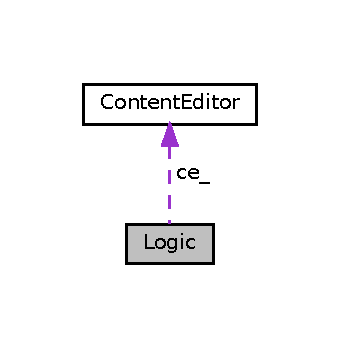
\includegraphics[width=268pt]{class_logic__coll__graph}
\end{center}
\end{figure}
\subsection*{Открытые члены}
\begin{DoxyCompactItemize}
\item 
\hyperlink{class_logic_a9fb0198e941a32f25cb110875751f78e}{Logic} (Q\+Plain\+Text\+Edit $\ast$output)
\item 
\hyperlink{class_logic_a406131db5b87e8d4b396aec37f3c1f69}{$\sim$\+Logic} ()
\item 
void \hyperlink{class_logic_af592736369fd989be41c59b4e7315ab5}{set\+Vars} (Q\+List$<$ Q\+String $>$ $\ast$v)
\begin{DoxyCompactList}\small\item\em \hyperlink{class_logic_af592736369fd989be41c59b4e7315ab5}{Logic\+::set\+Vars} Добавляет массив логических переменных в внутренний массив \end{DoxyCompactList}\item 
void \hyperlink{class_logic_a17bd98c66121d7739f11af12affdb64b}{compute} ()
\begin{DoxyCompactList}\small\item\em \hyperlink{class_logic_a17bd98c66121d7739f11af12affdb64b}{Logic\+::compute} Инициирует вычисления \end{DoxyCompactList}\item 
void \hyperlink{class_logic_a7eae2f1ccdc24932e795b33906b501b7}{compute\+Logical\+Action} (Q\+List$<$ Q\+String $>$ $\ast$v)
\begin{DoxyCompactList}\small\item\em \hyperlink{class_logic_a7eae2f1ccdc24932e795b33906b501b7}{Logic\+::compute\+Logical\+Action} Инициирует вычисление таблицы истинности \end{DoxyCompactList}\item 
Q\+List$<$ Q\+String $>$ \hyperlink{class_logic_a0887d38c17058d50c4d8a3b7a8fc44ac}{get\+Vars\+Title} () const
\begin{DoxyCompactList}\small\item\em \hyperlink{class_logic_a0887d38c17058d50c4d8a3b7a8fc44ac}{Logic\+::get\+Vars\+Title} Отдает массив имен логических переменных \end{DoxyCompactList}\item 
Q\+List$<$ Q\+List$<$ bool $>$ $>$ \hyperlink{class_logic_a42630bbe8bded25027014e9f0b2a085e}{get\+Vars\+Data} () const
\begin{DoxyCompactList}\small\item\em \hyperlink{class_logic_a42630bbe8bded25027014e9f0b2a085e}{Logic\+::get\+Vars\+Data} Отдает массив всех данных из логических переменных \end{DoxyCompactList}\item 
void \hyperlink{class_logic_a008dd758dde00f1f5940558f275ec216}{make\+S\+K\+NF} ()
\begin{DoxyCompactList}\small\item\em \hyperlink{class_logic_a008dd758dde00f1f5940558f275ec216}{Logic\+::make\+S\+K\+NF} создает Совершенную Конъюнктивную Нормальную Форму \end{DoxyCompactList}\item 
void \hyperlink{class_logic_a1494325c8d91b7fe5728b7dbdf82fca3}{make\+S\+D\+NF} ()
\begin{DoxyCompactList}\small\item\em \hyperlink{class_logic_a1494325c8d91b7fe5728b7dbdf82fca3}{Logic\+::make\+S\+D\+NF} создает Совершенную Дизъюнктивную Нормальную Форму \end{DoxyCompactList}\end{DoxyCompactItemize}
\subsection*{Открытые атрибуты}
\begin{DoxyCompactItemize}
\item 
const Q\+Map$<$ Q\+String, Q\+String $>$ \hyperlink{class_logic_a87779b9da5a43f388cbb26982502e989}{B\+I\+N\+A\+R\+Y\+\_\+\+O\+P\+E\+R\+A\+T\+I\+O\+N\+S\+\_\+}
\begin{DoxyCompactList}\small\item\em Используется для управление полем вывода \end{DoxyCompactList}\item 
const Q\+Map$<$ Q\+String, int $>$ \hyperlink{class_logic_a80a5ac2ef983887c55d5b64e941b9dbe}{B\+I\+N\+A\+R\+Y\+\_\+\+O\+P\+E\+R\+A\+T\+I\+O\+N\+S\+\_\+\+T\+O\+\_\+\+N\+U\+M\+\_\+}
\begin{DoxyCompactList}\small\item\em Словарь бинарных операций \end{DoxyCompactList}\item 
const Q\+List$<$ Q\+String $>$ \hyperlink{class_logic_a5d00b20d2c2a531f8796581f49fa7d5a}{A\+V\+I\+A\+B\+L\+E\+\_\+\+N\+A\+M\+E\+\_\+\+O\+F\+\_\+\+V\+A\+R\+S\+\_\+}
\begin{DoxyCompactList}\small\item\em Сопоставление бинарной операции с её внутренним номером (нужно для удобства) \end{DoxyCompactList}\end{DoxyCompactItemize}


\subsection{Подробное описание}
\hyperlink{class_logic}{Logic} -\/ Класс отвечает за логику выполнения действий 

\subsection{Конструктор(ы)}
\mbox{\Hypertarget{class_logic_a9fb0198e941a32f25cb110875751f78e}\label{class_logic_a9fb0198e941a32f25cb110875751f78e}} 
\index{Logic@{Logic}!Logic@{Logic}}
\index{Logic@{Logic}!Logic@{Logic}}
\subsubsection{\texorpdfstring{Logic()}{Logic()}}
{\footnotesize\ttfamily Logic\+::\+Logic (\begin{DoxyParamCaption}\item[{Q\+Plain\+Text\+Edit $\ast$}]{output }\end{DoxyParamCaption})}

\mbox{\Hypertarget{class_logic_a406131db5b87e8d4b396aec37f3c1f69}\label{class_logic_a406131db5b87e8d4b396aec37f3c1f69}} 
\index{Logic@{Logic}!````~Logic@{$\sim$\+Logic}}
\index{````~Logic@{$\sim$\+Logic}!Logic@{Logic}}
\subsubsection{\texorpdfstring{$\sim$\+Logic()}{~Logic()}}
{\footnotesize\ttfamily Logic\+::$\sim$\+Logic (\begin{DoxyParamCaption}{ }\end{DoxyParamCaption})}



\subsection{Методы}
\mbox{\Hypertarget{class_logic_a17bd98c66121d7739f11af12affdb64b}\label{class_logic_a17bd98c66121d7739f11af12affdb64b}} 
\index{Logic@{Logic}!compute@{compute}}
\index{compute@{compute}!Logic@{Logic}}
\subsubsection{\texorpdfstring{compute()}{compute()}}
{\footnotesize\ttfamily void Logic\+::compute (\begin{DoxyParamCaption}{ }\end{DoxyParamCaption})}



\hyperlink{class_logic_a17bd98c66121d7739f11af12affdb64b}{Logic\+::compute} Инициирует вычисления 

Граф вызовов\+:\nopagebreak
\begin{figure}[H]
\begin{center}
\leavevmode
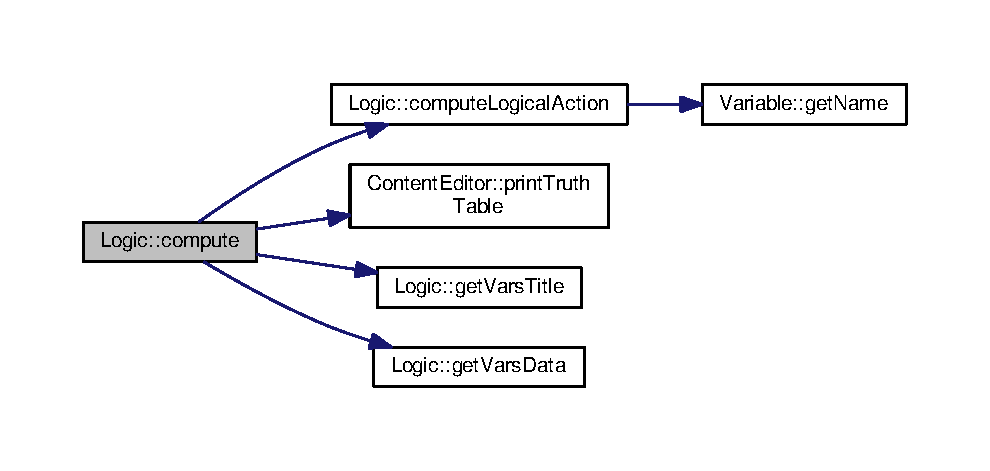
\includegraphics[width=350pt]{class_logic_a17bd98c66121d7739f11af12affdb64b_cgraph}
\end{center}
\end{figure}
Граф вызова функции\+:\nopagebreak
\begin{figure}[H]
\begin{center}
\leavevmode
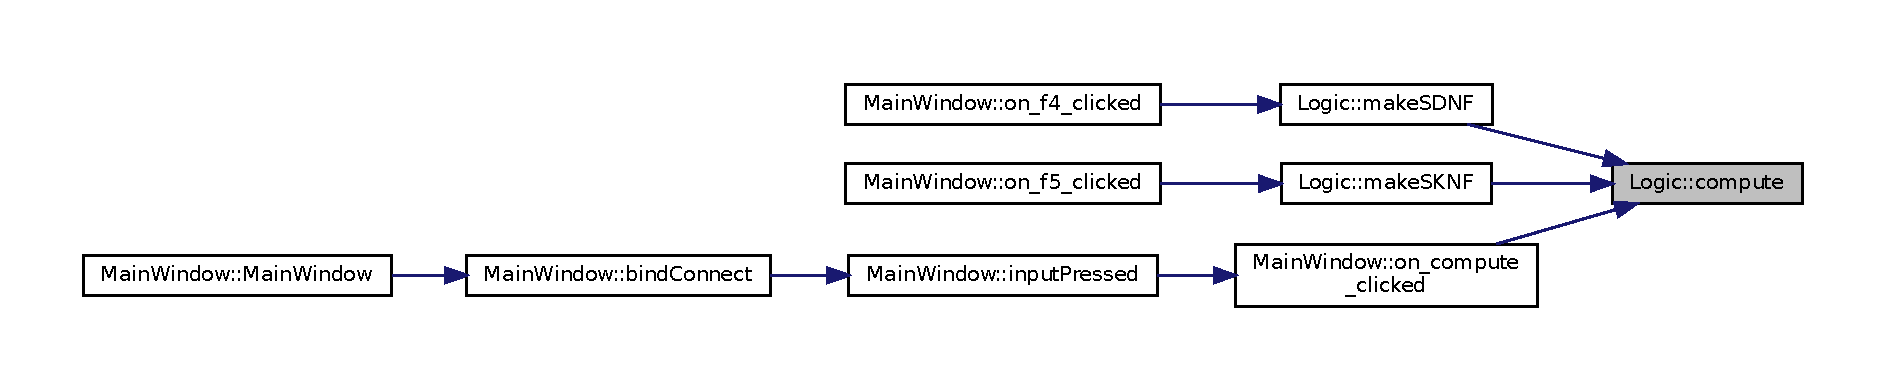
\includegraphics[width=350pt]{class_logic_a17bd98c66121d7739f11af12affdb64b_icgraph}
\end{center}
\end{figure}
\mbox{\Hypertarget{class_logic_a7eae2f1ccdc24932e795b33906b501b7}\label{class_logic_a7eae2f1ccdc24932e795b33906b501b7}} 
\index{Logic@{Logic}!compute\+Logical\+Action@{compute\+Logical\+Action}}
\index{compute\+Logical\+Action@{compute\+Logical\+Action}!Logic@{Logic}}
\subsubsection{\texorpdfstring{compute\+Logical\+Action()}{computeLogicalAction()}}
{\footnotesize\ttfamily void Logic\+::compute\+Logical\+Action (\begin{DoxyParamCaption}\item[{Q\+List$<$ Q\+String $>$ $\ast$}]{v }\end{DoxyParamCaption})}



\hyperlink{class_logic_a7eae2f1ccdc24932e795b33906b501b7}{Logic\+::compute\+Logical\+Action} Инициирует вычисление таблицы истинности 


\begin{DoxyParams}{Аргументы}
{\em v} & указатель на строки с логическими действиями \\
\hline
\end{DoxyParams}
Граф вызовов\+:\nopagebreak
\begin{figure}[H]
\begin{center}
\leavevmode
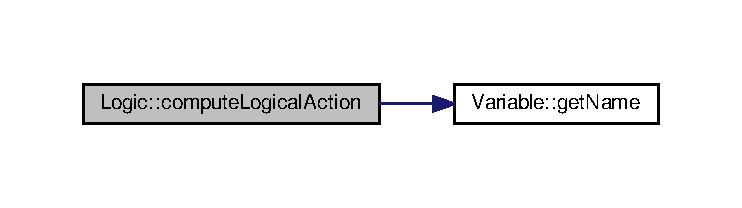
\includegraphics[width=350pt]{class_logic_a7eae2f1ccdc24932e795b33906b501b7_cgraph}
\end{center}
\end{figure}
Граф вызова функции\+:\nopagebreak
\begin{figure}[H]
\begin{center}
\leavevmode
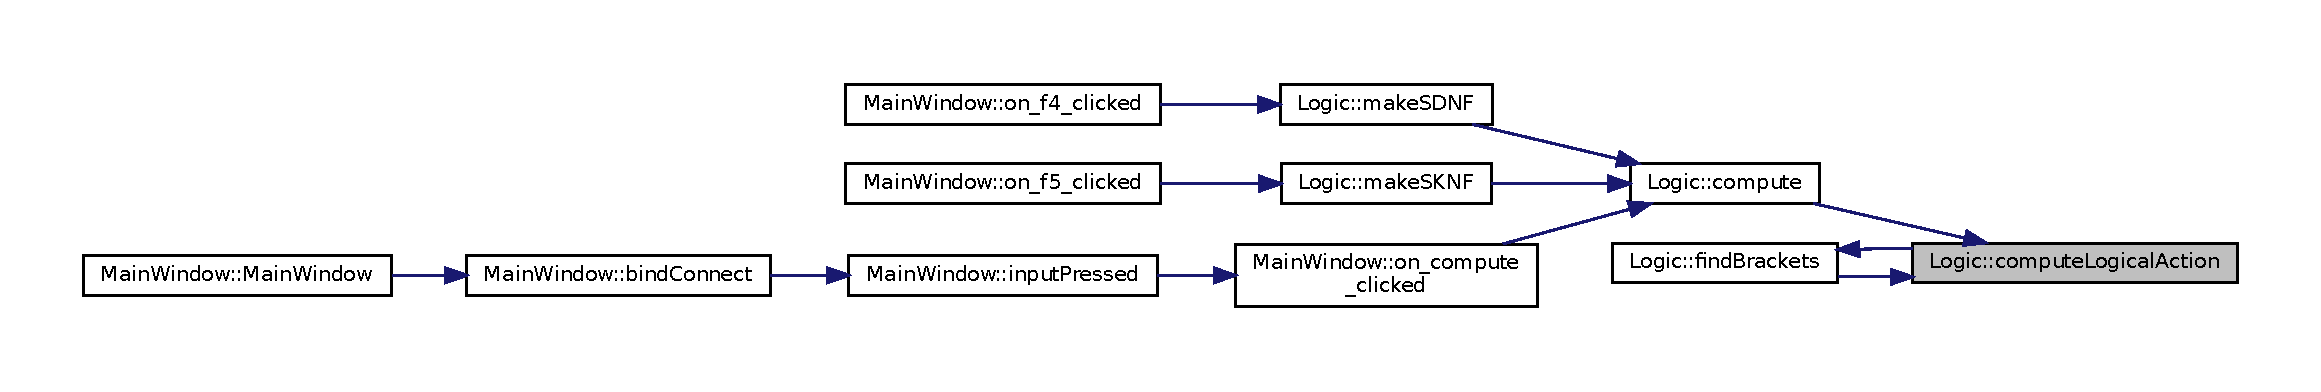
\includegraphics[width=350pt]{class_logic_a7eae2f1ccdc24932e795b33906b501b7_icgraph}
\end{center}
\end{figure}
\mbox{\Hypertarget{class_logic_a42630bbe8bded25027014e9f0b2a085e}\label{class_logic_a42630bbe8bded25027014e9f0b2a085e}} 
\index{Logic@{Logic}!get\+Vars\+Data@{get\+Vars\+Data}}
\index{get\+Vars\+Data@{get\+Vars\+Data}!Logic@{Logic}}
\subsubsection{\texorpdfstring{get\+Vars\+Data()}{getVarsData()}}
{\footnotesize\ttfamily Q\+List$<$ Q\+List$<$ bool $>$ $>$ Logic\+::get\+Vars\+Data (\begin{DoxyParamCaption}{ }\end{DoxyParamCaption}) const}



\hyperlink{class_logic_a42630bbe8bded25027014e9f0b2a085e}{Logic\+::get\+Vars\+Data} Отдает массив всех данных из логических переменных 

\begin{DoxyReturn}{Возвращает}
все данные из логических переменных 
\end{DoxyReturn}
Граф вызова функции\+:\nopagebreak
\begin{figure}[H]
\begin{center}
\leavevmode
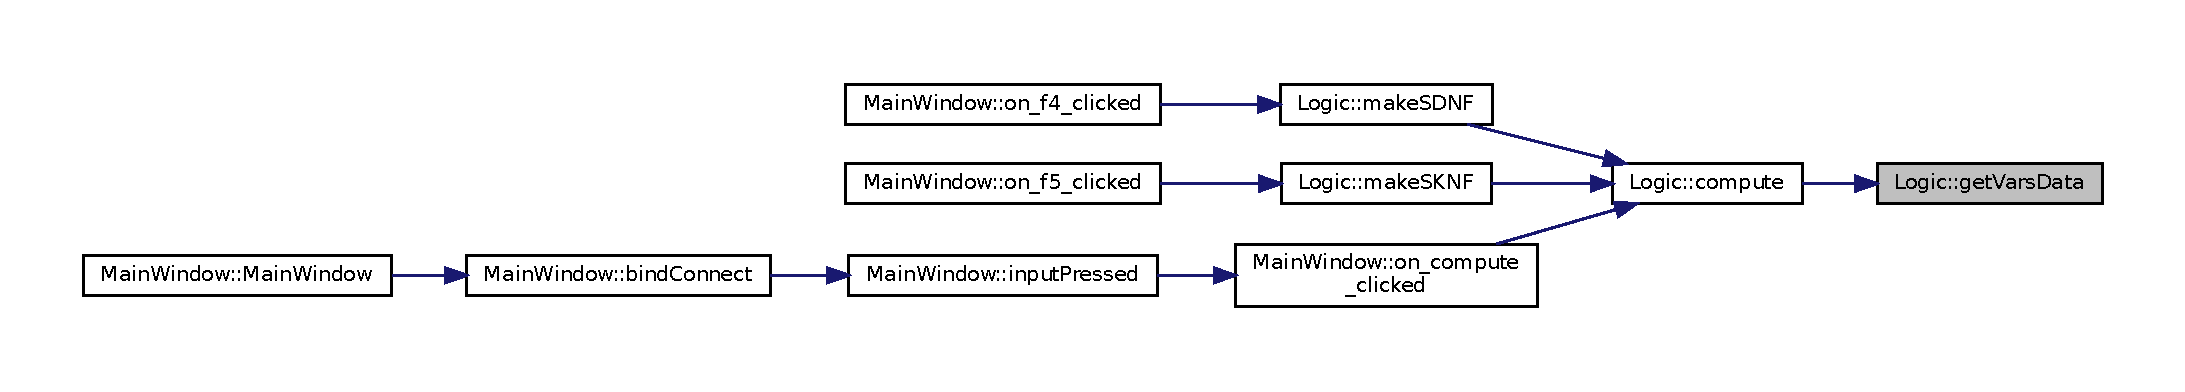
\includegraphics[width=350pt]{class_logic_a42630bbe8bded25027014e9f0b2a085e_icgraph}
\end{center}
\end{figure}
\mbox{\Hypertarget{class_logic_a0887d38c17058d50c4d8a3b7a8fc44ac}\label{class_logic_a0887d38c17058d50c4d8a3b7a8fc44ac}} 
\index{Logic@{Logic}!get\+Vars\+Title@{get\+Vars\+Title}}
\index{get\+Vars\+Title@{get\+Vars\+Title}!Logic@{Logic}}
\subsubsection{\texorpdfstring{get\+Vars\+Title()}{getVarsTitle()}}
{\footnotesize\ttfamily Q\+List$<$ Q\+String $>$ Logic\+::get\+Vars\+Title (\begin{DoxyParamCaption}{ }\end{DoxyParamCaption}) const}



\hyperlink{class_logic_a0887d38c17058d50c4d8a3b7a8fc44ac}{Logic\+::get\+Vars\+Title} Отдает массив имен логических переменных 

\begin{DoxyReturn}{Возвращает}
массив имен логических переменных 
\end{DoxyReturn}
Граф вызова функции\+:\nopagebreak
\begin{figure}[H]
\begin{center}
\leavevmode
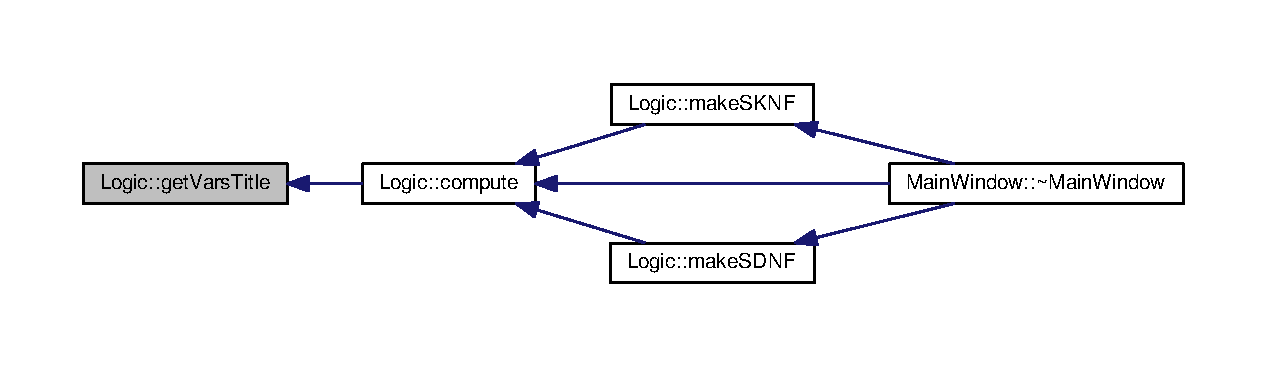
\includegraphics[width=350pt]{class_logic_a0887d38c17058d50c4d8a3b7a8fc44ac_icgraph}
\end{center}
\end{figure}
\mbox{\Hypertarget{class_logic_a1494325c8d91b7fe5728b7dbdf82fca3}\label{class_logic_a1494325c8d91b7fe5728b7dbdf82fca3}} 
\index{Logic@{Logic}!make\+S\+D\+NF@{make\+S\+D\+NF}}
\index{make\+S\+D\+NF@{make\+S\+D\+NF}!Logic@{Logic}}
\subsubsection{\texorpdfstring{make\+S\+D\+N\+F()}{makeSDNF()}}
{\footnotesize\ttfamily void Logic\+::make\+S\+D\+NF (\begin{DoxyParamCaption}{ }\end{DoxyParamCaption})}



\hyperlink{class_logic_a1494325c8d91b7fe5728b7dbdf82fca3}{Logic\+::make\+S\+D\+NF} создает Совершенную Дизъюнктивную Нормальную Форму 

Граф вызовов\+:\nopagebreak
\begin{figure}[H]
\begin{center}
\leavevmode
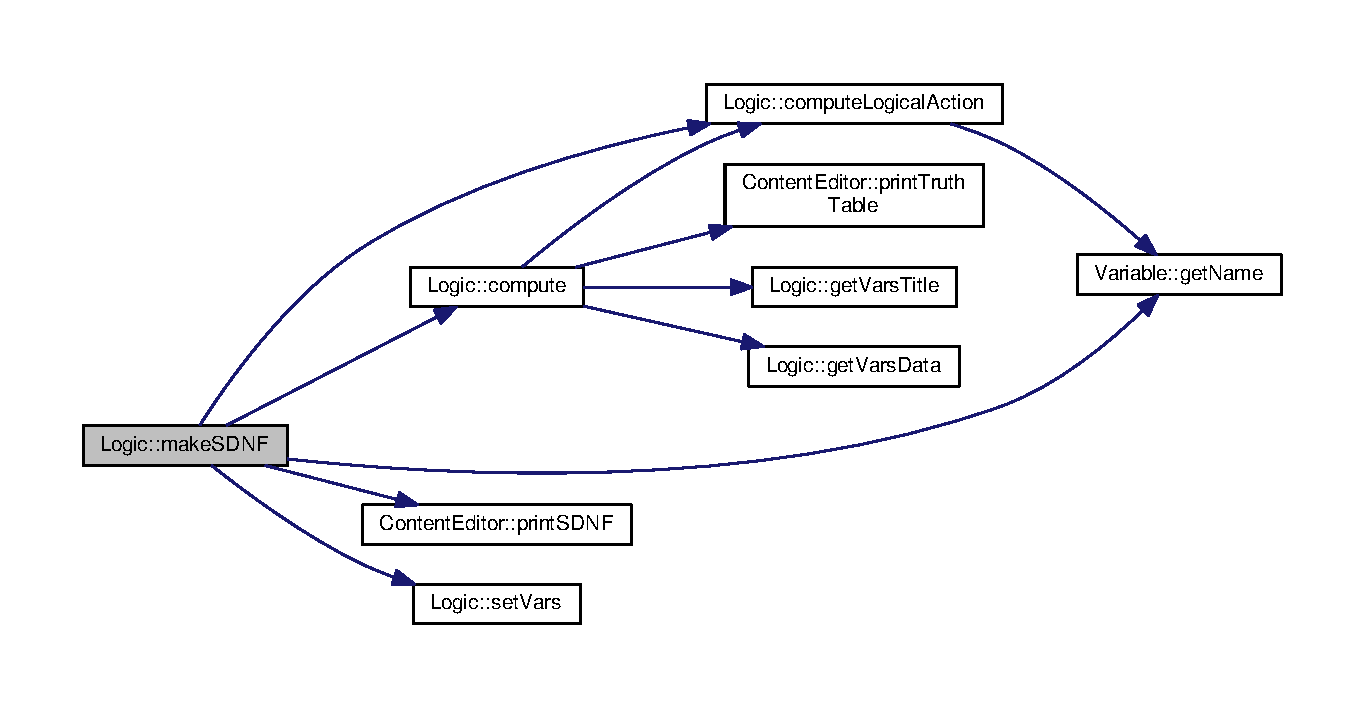
\includegraphics[width=350pt]{class_logic_a1494325c8d91b7fe5728b7dbdf82fca3_cgraph}
\end{center}
\end{figure}
Граф вызова функции\+:\nopagebreak
\begin{figure}[H]
\begin{center}
\leavevmode
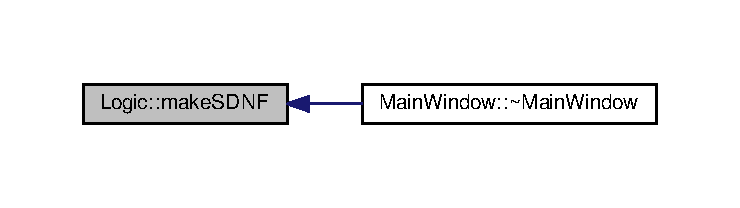
\includegraphics[width=350pt]{class_logic_a1494325c8d91b7fe5728b7dbdf82fca3_icgraph}
\end{center}
\end{figure}
\mbox{\Hypertarget{class_logic_a008dd758dde00f1f5940558f275ec216}\label{class_logic_a008dd758dde00f1f5940558f275ec216}} 
\index{Logic@{Logic}!make\+S\+K\+NF@{make\+S\+K\+NF}}
\index{make\+S\+K\+NF@{make\+S\+K\+NF}!Logic@{Logic}}
\subsubsection{\texorpdfstring{make\+S\+K\+N\+F()}{makeSKNF()}}
{\footnotesize\ttfamily void Logic\+::make\+S\+K\+NF (\begin{DoxyParamCaption}{ }\end{DoxyParamCaption})}



\hyperlink{class_logic_a008dd758dde00f1f5940558f275ec216}{Logic\+::make\+S\+K\+NF} создает Совершенную Конъюнктивную Нормальную Форму 

Граф вызовов\+:\nopagebreak
\begin{figure}[H]
\begin{center}
\leavevmode
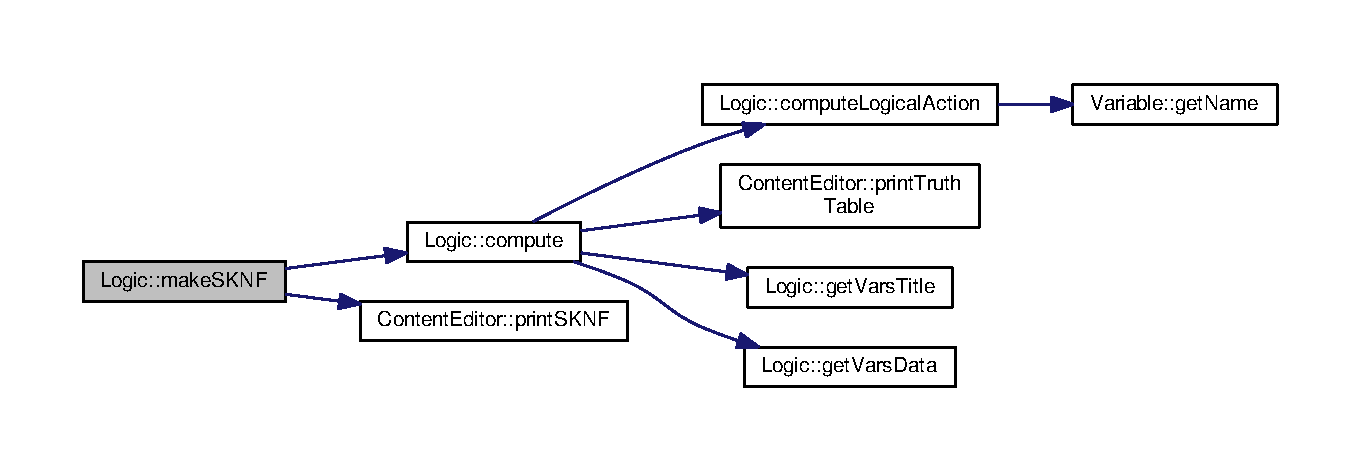
\includegraphics[width=350pt]{class_logic_a008dd758dde00f1f5940558f275ec216_cgraph}
\end{center}
\end{figure}
Граф вызова функции\+:\nopagebreak
\begin{figure}[H]
\begin{center}
\leavevmode
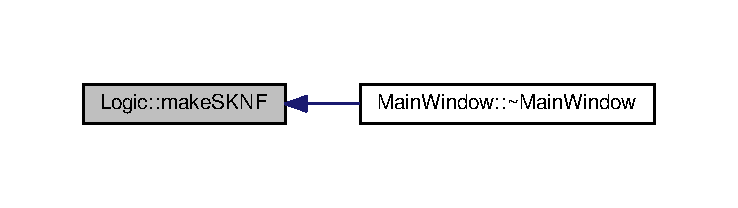
\includegraphics[width=350pt]{class_logic_a008dd758dde00f1f5940558f275ec216_icgraph}
\end{center}
\end{figure}
\mbox{\Hypertarget{class_logic_af592736369fd989be41c59b4e7315ab5}\label{class_logic_af592736369fd989be41c59b4e7315ab5}} 
\index{Logic@{Logic}!set\+Vars@{set\+Vars}}
\index{set\+Vars@{set\+Vars}!Logic@{Logic}}
\subsubsection{\texorpdfstring{set\+Vars()}{setVars()}}
{\footnotesize\ttfamily void Logic\+::set\+Vars (\begin{DoxyParamCaption}\item[{Q\+List$<$ Q\+String $>$ $\ast$}]{v }\end{DoxyParamCaption})}



\hyperlink{class_logic_af592736369fd989be41c59b4e7315ab5}{Logic\+::set\+Vars} Добавляет массив логических переменных в внутренний массив 


\begin{DoxyParams}{Аргументы}
{\em v} & массив логических переменных \\
\hline
\end{DoxyParams}
Граф вызова функции\+:\nopagebreak
\begin{figure}[H]
\begin{center}
\leavevmode
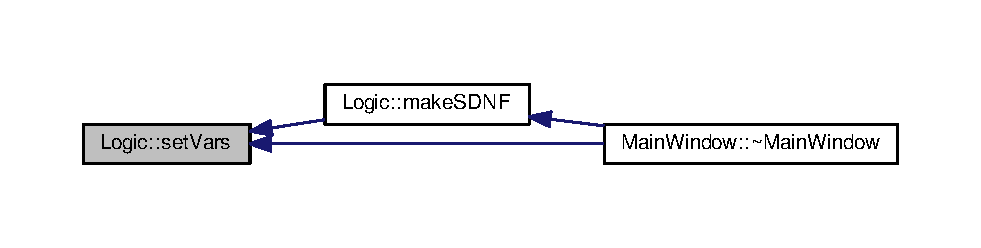
\includegraphics[width=350pt]{class_logic_af592736369fd989be41c59b4e7315ab5_icgraph}
\end{center}
\end{figure}


\subsection{Данные класса}
\mbox{\Hypertarget{class_logic_a5d00b20d2c2a531f8796581f49fa7d5a}\label{class_logic_a5d00b20d2c2a531f8796581f49fa7d5a}} 
\index{Logic@{Logic}!A\+V\+I\+A\+B\+L\+E\+\_\+\+N\+A\+M\+E\+\_\+\+O\+F\+\_\+\+V\+A\+R\+S\+\_\+@{A\+V\+I\+A\+B\+L\+E\+\_\+\+N\+A\+M\+E\+\_\+\+O\+F\+\_\+\+V\+A\+R\+S\+\_\+}}
\index{A\+V\+I\+A\+B\+L\+E\+\_\+\+N\+A\+M\+E\+\_\+\+O\+F\+\_\+\+V\+A\+R\+S\+\_\+@{A\+V\+I\+A\+B\+L\+E\+\_\+\+N\+A\+M\+E\+\_\+\+O\+F\+\_\+\+V\+A\+R\+S\+\_\+}!Logic@{Logic}}
\subsubsection{\texorpdfstring{A\+V\+I\+A\+B\+L\+E\+\_\+\+N\+A\+M\+E\+\_\+\+O\+F\+\_\+\+V\+A\+R\+S\+\_\+}{AVIABLE\_NAME\_OF\_VARS\_}}
{\footnotesize\ttfamily const Q\+List$<$Q\+String$>$ Logic\+::\+A\+V\+I\+A\+B\+L\+E\+\_\+\+N\+A\+M\+E\+\_\+\+O\+F\+\_\+\+V\+A\+R\+S\+\_\+}

{\bfseries Инициализатор}
\begin{DoxyCode}
\{
        \textcolor{stringliteral}{"A"}, \textcolor{stringliteral}{"B"}, \textcolor{stringliteral}{"C"}, \textcolor{stringliteral}{"D"}, \textcolor{stringliteral}{"E"}, \textcolor{stringliteral}{"F"}, \textcolor{stringliteral}{"G"}, \textcolor{stringliteral}{"X"}, \textcolor{stringliteral}{"Y"}, \textcolor{stringliteral}{"Z"},
        \textcolor{stringliteral}{"a"}, \textcolor{stringliteral}{"b"}, \textcolor{stringliteral}{"c"}, \textcolor{stringliteral}{"d"}, \textcolor{stringliteral}{"e"}, \textcolor{stringliteral}{"f"}, \textcolor{stringliteral}{"g"}, \textcolor{stringliteral}{"x"}, \textcolor{stringliteral}{"y"}, \textcolor{stringliteral}{"z"}
    \}
\end{DoxyCode}


Сопоставление бинарной операции с её внутренним номером (нужно для удобства) 

\mbox{\Hypertarget{class_logic_a87779b9da5a43f388cbb26982502e989}\label{class_logic_a87779b9da5a43f388cbb26982502e989}} 
\index{Logic@{Logic}!B\+I\+N\+A\+R\+Y\+\_\+\+O\+P\+E\+R\+A\+T\+I\+O\+N\+S\+\_\+@{B\+I\+N\+A\+R\+Y\+\_\+\+O\+P\+E\+R\+A\+T\+I\+O\+N\+S\+\_\+}}
\index{B\+I\+N\+A\+R\+Y\+\_\+\+O\+P\+E\+R\+A\+T\+I\+O\+N\+S\+\_\+@{B\+I\+N\+A\+R\+Y\+\_\+\+O\+P\+E\+R\+A\+T\+I\+O\+N\+S\+\_\+}!Logic@{Logic}}
\subsubsection{\texorpdfstring{B\+I\+N\+A\+R\+Y\+\_\+\+O\+P\+E\+R\+A\+T\+I\+O\+N\+S\+\_\+}{BINARY\_OPERATIONS\_}}
{\footnotesize\ttfamily const Q\+Map$<$Q\+String, Q\+String$>$ Logic\+::\+B\+I\+N\+A\+R\+Y\+\_\+\+O\+P\+E\+R\+A\+T\+I\+O\+N\+S\+\_\+}

{\bfseries Инициализатор}
\begin{DoxyCode}
\{
        \{\textcolor{stringliteral}{"*"}, \textcolor{stringliteral}{"conjunction"}\},
        \{\textcolor{stringliteral}{"+"}, \textcolor{stringliteral}{"disjunction"}\},
        \{\textcolor{stringliteral}{"^"}, \textcolor{stringliteral}{"exclusiveDisjunction"}\},
        \{\textcolor{stringliteral}{"|"}, \textcolor{stringliteral}{"notAnd"}\},
        \{\textcolor{stringliteral}{"#"}, \textcolor{stringliteral}{"notOr"}\},
        \{\textcolor{stringliteral}{"->"}, \textcolor{stringliteral}{"implication"}\},
        \{\textcolor{stringliteral}{"<-"}, \textcolor{stringliteral}{"converse"}\},
        \{\textcolor{stringliteral}{"~"}, \textcolor{stringliteral}{"equivalent"}\}
    \}
\end{DoxyCode}


Используется для управление полем вывода 

\mbox{\Hypertarget{class_logic_a80a5ac2ef983887c55d5b64e941b9dbe}\label{class_logic_a80a5ac2ef983887c55d5b64e941b9dbe}} 
\index{Logic@{Logic}!B\+I\+N\+A\+R\+Y\+\_\+\+O\+P\+E\+R\+A\+T\+I\+O\+N\+S\+\_\+\+T\+O\+\_\+\+N\+U\+M\+\_\+@{B\+I\+N\+A\+R\+Y\+\_\+\+O\+P\+E\+R\+A\+T\+I\+O\+N\+S\+\_\+\+T\+O\+\_\+\+N\+U\+M\+\_\+}}
\index{B\+I\+N\+A\+R\+Y\+\_\+\+O\+P\+E\+R\+A\+T\+I\+O\+N\+S\+\_\+\+T\+O\+\_\+\+N\+U\+M\+\_\+@{B\+I\+N\+A\+R\+Y\+\_\+\+O\+P\+E\+R\+A\+T\+I\+O\+N\+S\+\_\+\+T\+O\+\_\+\+N\+U\+M\+\_\+}!Logic@{Logic}}
\subsubsection{\texorpdfstring{B\+I\+N\+A\+R\+Y\+\_\+\+O\+P\+E\+R\+A\+T\+I\+O\+N\+S\+\_\+\+T\+O\+\_\+\+N\+U\+M\+\_\+}{BINARY\_OPERATIONS\_TO\_NUM\_}}
{\footnotesize\ttfamily const Q\+Map$<$Q\+String, int$>$ Logic\+::\+B\+I\+N\+A\+R\+Y\+\_\+\+O\+P\+E\+R\+A\+T\+I\+O\+N\+S\+\_\+\+T\+O\+\_\+\+N\+U\+M\+\_\+}

{\bfseries Инициализатор}
\begin{DoxyCode}
\{
        \{\textcolor{stringliteral}{"conjunction"}, 1\},
        \{\textcolor{stringliteral}{"disjunction"}, 2\},
        \{\textcolor{stringliteral}{"implication"}, 3\},
        \{\textcolor{stringliteral}{"converse"}, 4\},
        \{\textcolor{stringliteral}{"equivalent"}, 5\},
        \{\textcolor{stringliteral}{"exclusiveDisjunction"}, 6\},
        \{\textcolor{stringliteral}{"notAnd"}, 7\},
        \{\textcolor{stringliteral}{"notOr"}, 8\}
    \}
\end{DoxyCode}


Словарь бинарных операций 



Объявления и описания членов классов находятся в файлах\+:\begin{DoxyCompactItemize}
\item 
/home/itain/\+Qt\+Projects/logic\+\_\+calculator/\hyperlink{logic_8h}{logic.\+h}\item 
/home/itain/\+Qt\+Projects/logic\+\_\+calculator/\hyperlink{logic_8cpp}{logic.\+cpp}\end{DoxyCompactItemize}

\hypertarget{class_main_window}{}\doxysection{Класс Main\+Window}
\label{class_main_window}\index{MainWindow@{MainWindow}}


\mbox{\hyperlink{class_main_window}{Main\+Window}} -\/ Класс отвечает за взаимодействие с пользовательским интерфейсом  




{\ttfamily \#include $<$mainwindow.\+h$>$}



Граф наследования\+:Main\+Window\+:\nopagebreak
\begin{figure}[H]
\begin{center}
\leavevmode
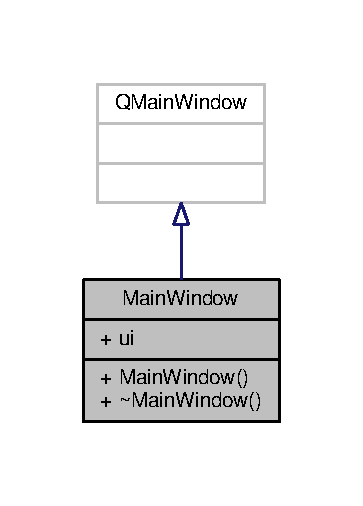
\includegraphics[width=167pt]{class_main_window__inherit__graph}
\end{center}
\end{figure}


Граф связей класса Main\+Window\+:\nopagebreak
\begin{figure}[H]
\begin{center}
\leavevmode
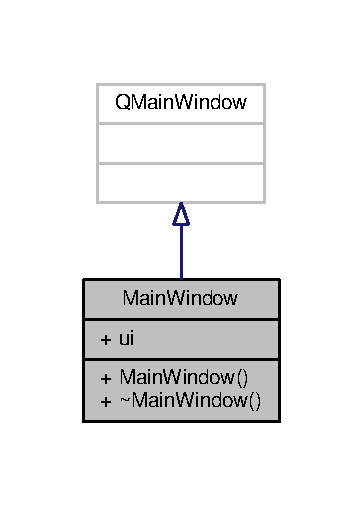
\includegraphics[width=336pt]{class_main_window__coll__graph}
\end{center}
\end{figure}
\doxysubsection*{Открытые члены}
\begin{DoxyCompactItemize}
\item 
\mbox{\hyperlink{class_main_window_a996c5a2b6f77944776856f08ec30858d}{Main\+Window}} (Q\+Widget $\ast$parent=nullptr)
\item 
\mbox{\hyperlink{class_main_window_ae98d00a93bc118200eeef9f9bba1dba7}{$\sim$\+Main\+Window}} ()
\end{DoxyCompactItemize}
\doxysubsection*{Открытые атрибуты}
\begin{DoxyCompactItemize}
\item 
Ui\+::\+Main\+Window $\ast$ \mbox{\hyperlink{class_main_window_a35466a70ed47252a0191168126a352a5}{ui}}
\end{DoxyCompactItemize}
\doxysubsection*{Закрытые слоты}
\begin{DoxyCompactItemize}
\item 
void \mbox{\hyperlink{class_main_window_ad2b196b4c7680e1995c870863ee3cabe}{input\+Pressed}} ()
\begin{DoxyCompactList}\small\item\em \mbox{\hyperlink{class_main_window_ad2b196b4c7680e1995c870863ee3cabe}{Main\+Window\+::input\+Pressed}} Обработчик для поля ввода данных, вызывается при нажатии на enter. \end{DoxyCompactList}\item 
void \mbox{\hyperlink{class_main_window_a35937dfc64e91849432cf75714cafcc7}{on\+Clicked}} ()
\begin{DoxyCompactList}\small\item\em \mbox{\hyperlink{class_main_window_a35937dfc64e91849432cf75714cafcc7}{Main\+Window\+::on\+Clicked}} Обработчик на кнопки логических операций. Добавляет в поле ввода данных соответствующий символ \end{DoxyCompactList}\item 
void \mbox{\hyperlink{class_main_window_afc3c47ba36b6793f5f86af1f8cf71f3b}{bind\+Connect}} () const
\begin{DoxyCompactList}\small\item\em \mbox{\hyperlink{class_main_window_afc3c47ba36b6793f5f86af1f8cf71f3b}{Main\+Window\+::bind\+Connect}} Создаёт связи между обработчиком события on\+Clicked и нажатой кнопкой \end{DoxyCompactList}\item 
void \mbox{\hyperlink{class_main_window_a41bad26e9dbaae6c92d2a076797ef33c}{on\+\_\+compute\+\_\+clicked}} ()
\begin{DoxyCompactList}\small\item\em \mbox{\hyperlink{class_main_window_a41bad26e9dbaae6c92d2a076797ef33c}{Main\+Window\+::on\+\_\+compute\+\_\+clicked}} Обработчик нажатия на кнопку Вычислить \end{DoxyCompactList}\item 
void \mbox{\hyperlink{class_main_window_a9823fb93ccc1255eb7c4a749478a74a6}{on\+\_\+f5\+\_\+clicked}} ()
\begin{DoxyCompactList}\small\item\em \mbox{\hyperlink{class_main_window_a9823fb93ccc1255eb7c4a749478a74a6}{Main\+Window\+::on\+\_\+f5\+\_\+clicked}} Обработчик для кнопки СКНФ \end{DoxyCompactList}\item 
void \mbox{\hyperlink{class_main_window_af483459fc458b993949c504e1e0d24af}{on\+\_\+f4\+\_\+clicked}} ()
\begin{DoxyCompactList}\small\item\em \mbox{\hyperlink{class_main_window_af483459fc458b993949c504e1e0d24af}{Main\+Window\+::on\+\_\+f4\+\_\+clicked}} Обработчик для кнопки СДНФ \end{DoxyCompactList}\end{DoxyCompactItemize}
\doxysubsection*{Закрытые члены}
\begin{DoxyCompactItemize}
\item 
void \mbox{\hyperlink{class_main_window_a68da4ad6e2da6aad0b627612161a86dc}{connect\+Qss}} ()
\begin{DoxyCompactList}\small\item\em \mbox{\hyperlink{class_main_window_a68da4ad6e2da6aad0b627612161a86dc}{Main\+Window\+::connect\+Qss}} Отвечает за подключение стилей \end{DoxyCompactList}\end{DoxyCompactItemize}
\doxysubsection*{Закрытые данные}
\begin{DoxyCompactItemize}
\item 
\mbox{\hyperlink{class_input_editor}{Input\+Editor}} $\ast$ \mbox{\hyperlink{class_main_window_a44dcd3d3c75c90b005c644b26c58ac21}{ie\+\_\+}}
\item 
\mbox{\hyperlink{class_logic}{Logic}} $\ast$ \mbox{\hyperlink{class_main_window_a2362702e2f4888ead84da68a75c595d7}{logic\+\_\+}}
\begin{DoxyCompactList}\small\item\em отвечает за обработку данных, вводимых в поле ввода данных \end{DoxyCompactList}\end{DoxyCompactItemize}


\doxysubsection{Подробное описание}
\mbox{\hyperlink{class_main_window}{Main\+Window}} -\/ Класс отвечает за взаимодействие с пользовательским интерфейсом 

\doxysubsection{Конструктор(ы)}
\mbox{\Hypertarget{class_main_window_a996c5a2b6f77944776856f08ec30858d}\label{class_main_window_a996c5a2b6f77944776856f08ec30858d}} 
\index{MainWindow@{MainWindow}!MainWindow@{MainWindow}}
\index{MainWindow@{MainWindow}!MainWindow@{MainWindow}}
\doxysubsubsection{\texorpdfstring{MainWindow()}{MainWindow()}}
{\footnotesize\ttfamily Main\+Window\+::\+Main\+Window (\begin{DoxyParamCaption}\item[{Q\+Widget $\ast$}]{parent = {\ttfamily nullptr} }\end{DoxyParamCaption})\hspace{0.3cm}{\ttfamily [explicit]}}

Граф вызовов\+:\nopagebreak
\begin{figure}[H]
\begin{center}
\leavevmode
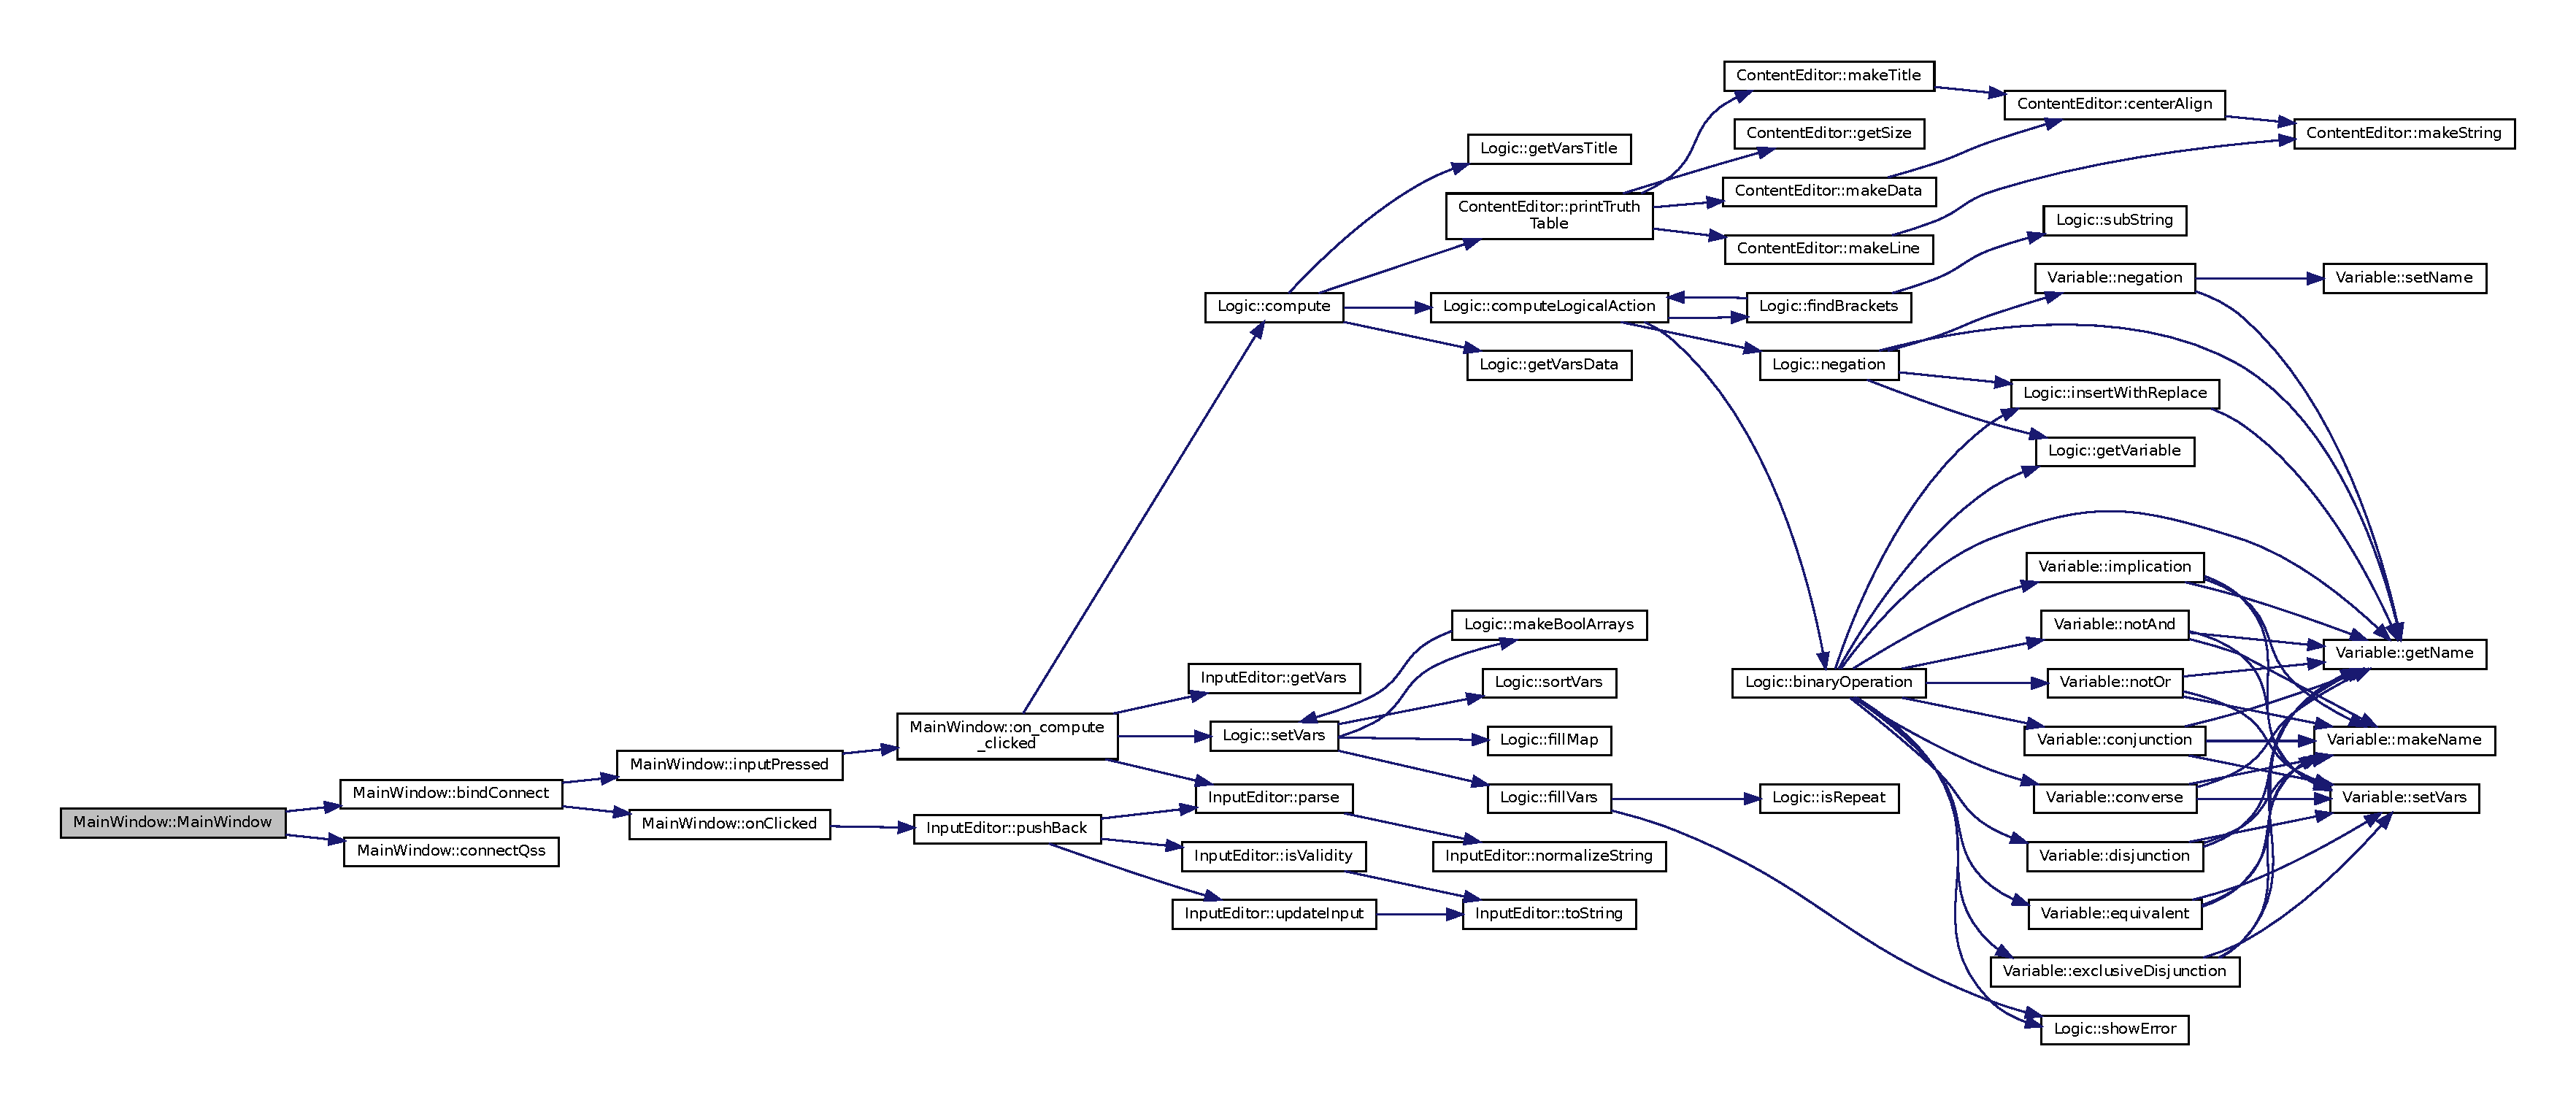
\includegraphics[width=350pt]{class_main_window_a996c5a2b6f77944776856f08ec30858d_cgraph}
\end{center}
\end{figure}
\mbox{\Hypertarget{class_main_window_ae98d00a93bc118200eeef9f9bba1dba7}\label{class_main_window_ae98d00a93bc118200eeef9f9bba1dba7}} 
\index{MainWindow@{MainWindow}!````~MainWindow@{$\sim$MainWindow}}
\index{````~MainWindow@{$\sim$MainWindow}!MainWindow@{MainWindow}}
\doxysubsubsection{\texorpdfstring{$\sim$MainWindow()}{~MainWindow()}}
{\footnotesize\ttfamily Main\+Window\+::$\sim$\+Main\+Window (\begin{DoxyParamCaption}{ }\end{DoxyParamCaption})}



\doxysubsection{Методы}
\mbox{\Hypertarget{class_main_window_afc3c47ba36b6793f5f86af1f8cf71f3b}\label{class_main_window_afc3c47ba36b6793f5f86af1f8cf71f3b}} 
\index{MainWindow@{MainWindow}!bindConnect@{bindConnect}}
\index{bindConnect@{bindConnect}!MainWindow@{MainWindow}}
\doxysubsubsection{\texorpdfstring{bindConnect}{bindConnect}}
{\footnotesize\ttfamily void Main\+Window\+::bind\+Connect (\begin{DoxyParamCaption}{ }\end{DoxyParamCaption}) const\hspace{0.3cm}{\ttfamily [private]}, {\ttfamily [slot]}}



\mbox{\hyperlink{class_main_window_afc3c47ba36b6793f5f86af1f8cf71f3b}{Main\+Window\+::bind\+Connect}} Создаёт связи между обработчиком события on\+Clicked и нажатой кнопкой 

Граф вызовов\+:\nopagebreak
\begin{figure}[H]
\begin{center}
\leavevmode
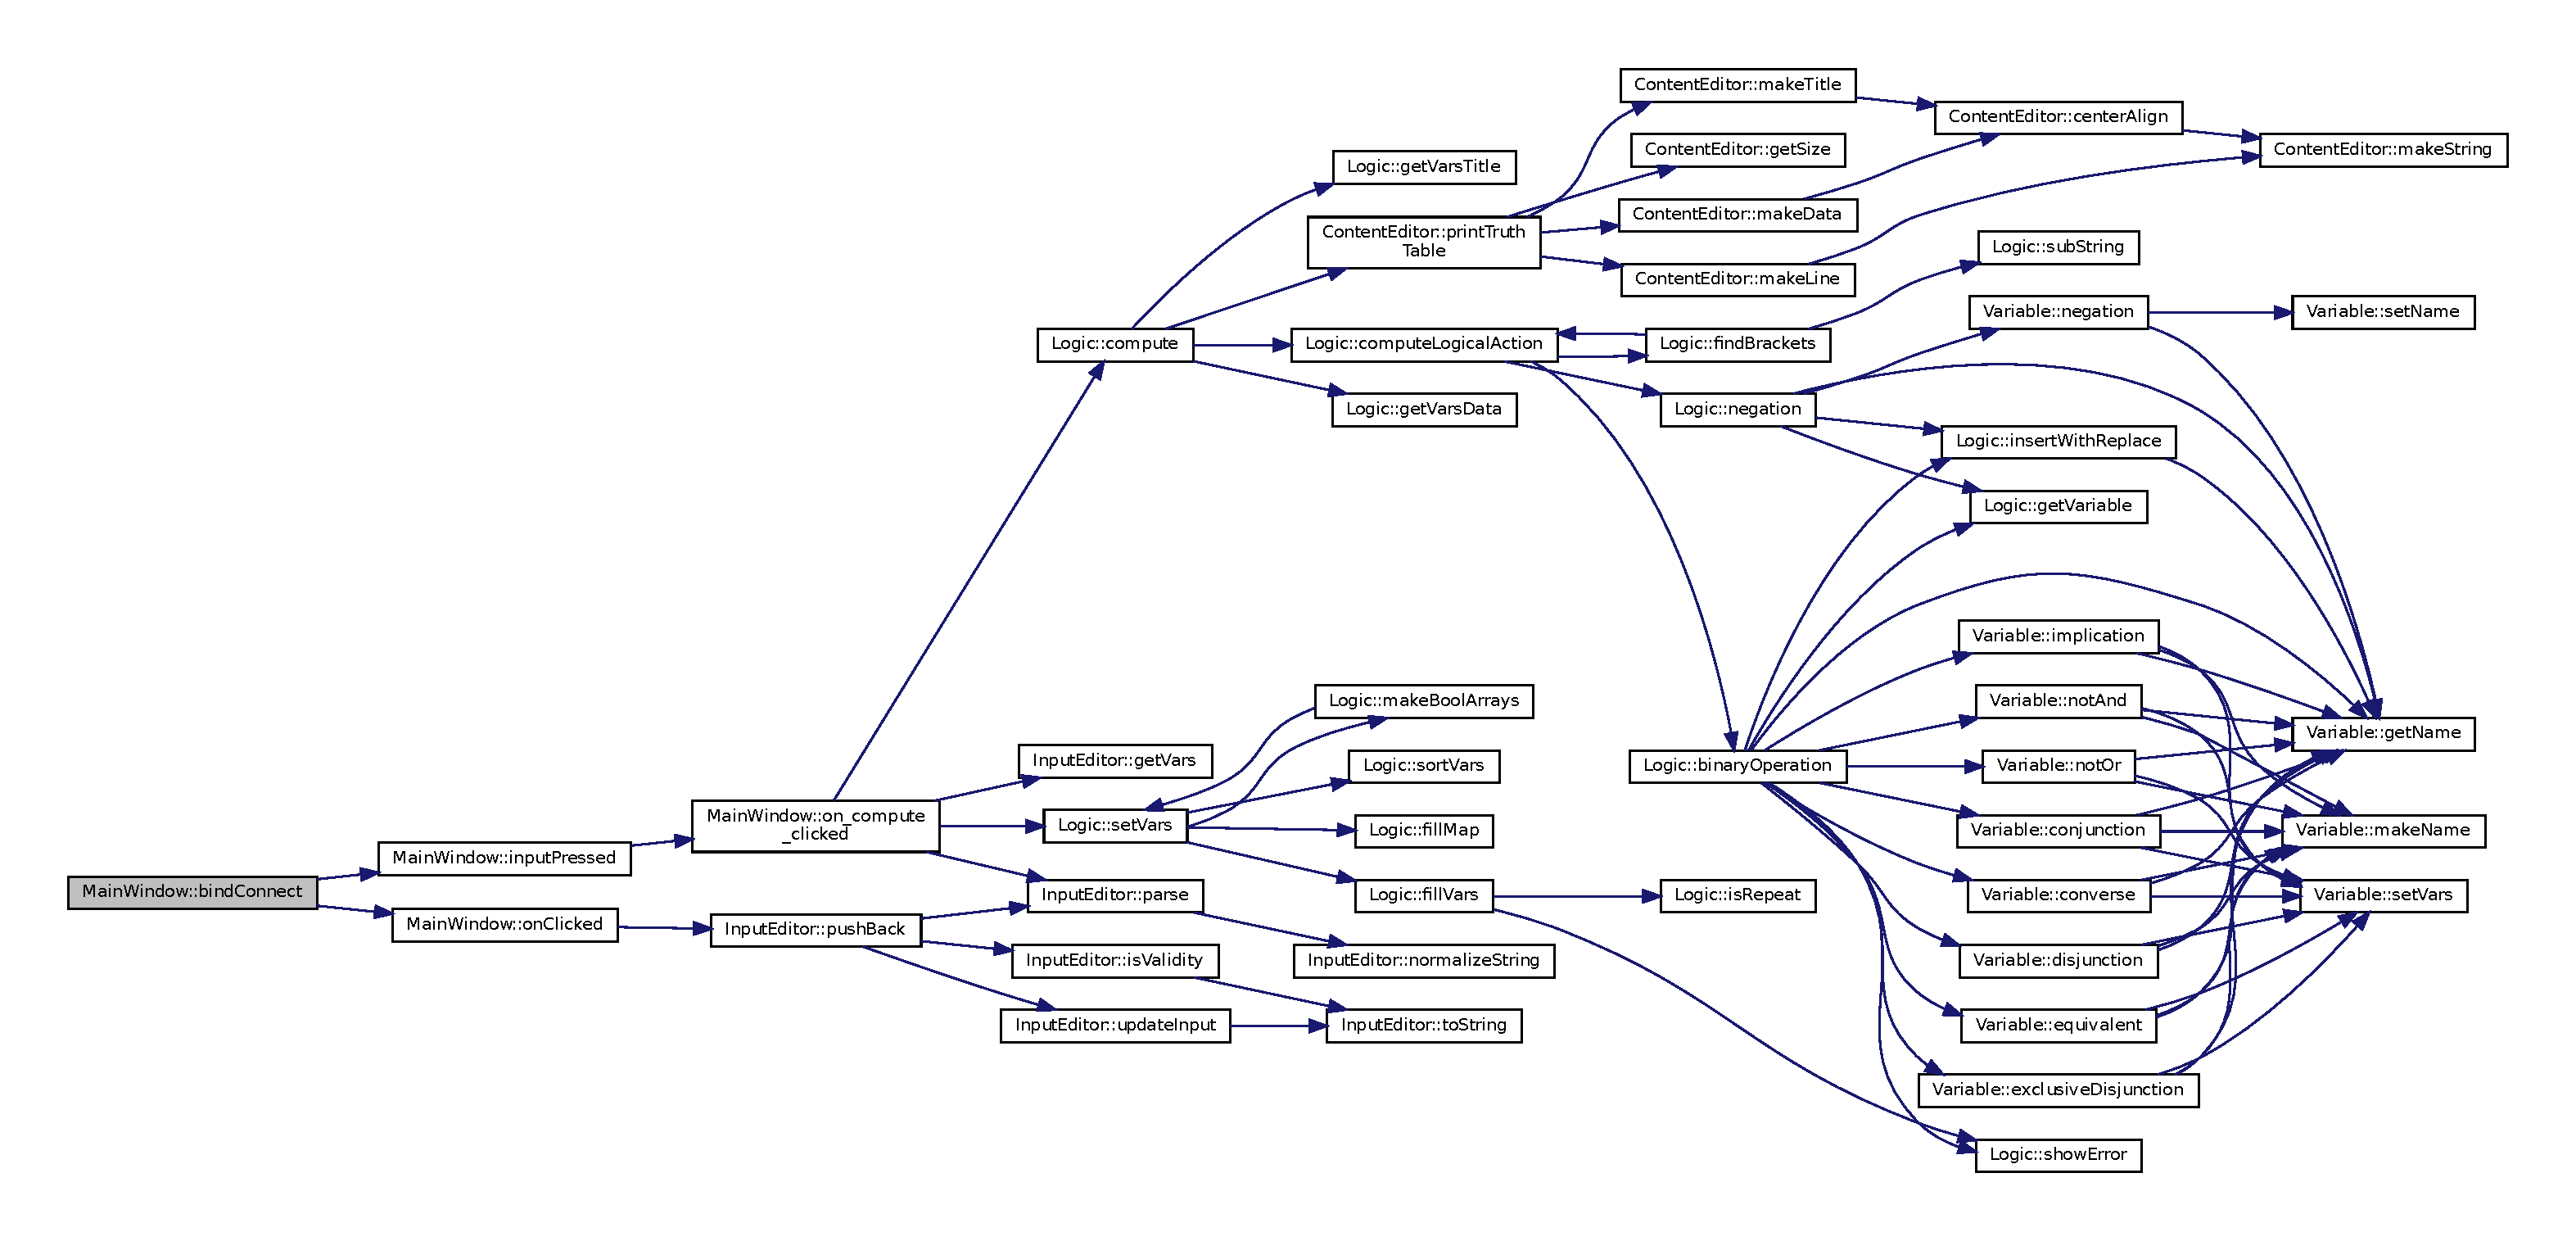
\includegraphics[width=350pt]{class_main_window_afc3c47ba36b6793f5f86af1f8cf71f3b_cgraph}
\end{center}
\end{figure}
Граф вызова функции\+:\nopagebreak
\begin{figure}[H]
\begin{center}
\leavevmode
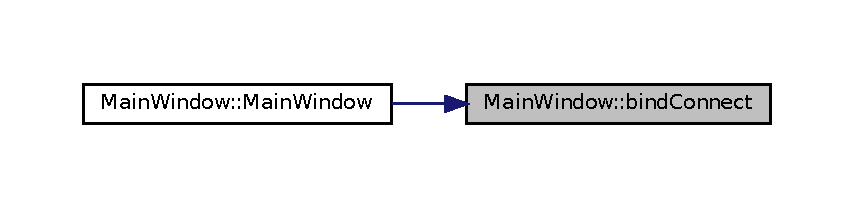
\includegraphics[width=350pt]{class_main_window_afc3c47ba36b6793f5f86af1f8cf71f3b_icgraph}
\end{center}
\end{figure}
\mbox{\Hypertarget{class_main_window_a68da4ad6e2da6aad0b627612161a86dc}\label{class_main_window_a68da4ad6e2da6aad0b627612161a86dc}} 
\index{MainWindow@{MainWindow}!connectQss@{connectQss}}
\index{connectQss@{connectQss}!MainWindow@{MainWindow}}
\doxysubsubsection{\texorpdfstring{connectQss()}{connectQss()}}
{\footnotesize\ttfamily void Main\+Window\+::connect\+Qss (\begin{DoxyParamCaption}{ }\end{DoxyParamCaption})\hspace{0.3cm}{\ttfamily [private]}}



\mbox{\hyperlink{class_main_window_a68da4ad6e2da6aad0b627612161a86dc}{Main\+Window\+::connect\+Qss}} Отвечает за подключение стилей 

Граф вызова функции\+:\nopagebreak
\begin{figure}[H]
\begin{center}
\leavevmode
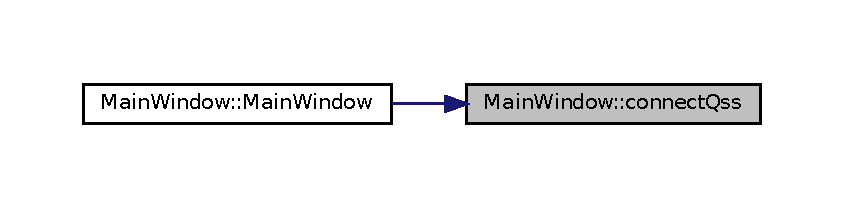
\includegraphics[width=350pt]{class_main_window_a68da4ad6e2da6aad0b627612161a86dc_icgraph}
\end{center}
\end{figure}
\mbox{\Hypertarget{class_main_window_ad2b196b4c7680e1995c870863ee3cabe}\label{class_main_window_ad2b196b4c7680e1995c870863ee3cabe}} 
\index{MainWindow@{MainWindow}!inputPressed@{inputPressed}}
\index{inputPressed@{inputPressed}!MainWindow@{MainWindow}}
\doxysubsubsection{\texorpdfstring{inputPressed}{inputPressed}}
{\footnotesize\ttfamily void Main\+Window\+::input\+Pressed (\begin{DoxyParamCaption}{ }\end{DoxyParamCaption})\hspace{0.3cm}{\ttfamily [private]}, {\ttfamily [slot]}}



\mbox{\hyperlink{class_main_window_ad2b196b4c7680e1995c870863ee3cabe}{Main\+Window\+::input\+Pressed}} Обработчик для поля ввода данных, вызывается при нажатии на enter. 

Граф вызовов\+:\nopagebreak
\begin{figure}[H]
\begin{center}
\leavevmode
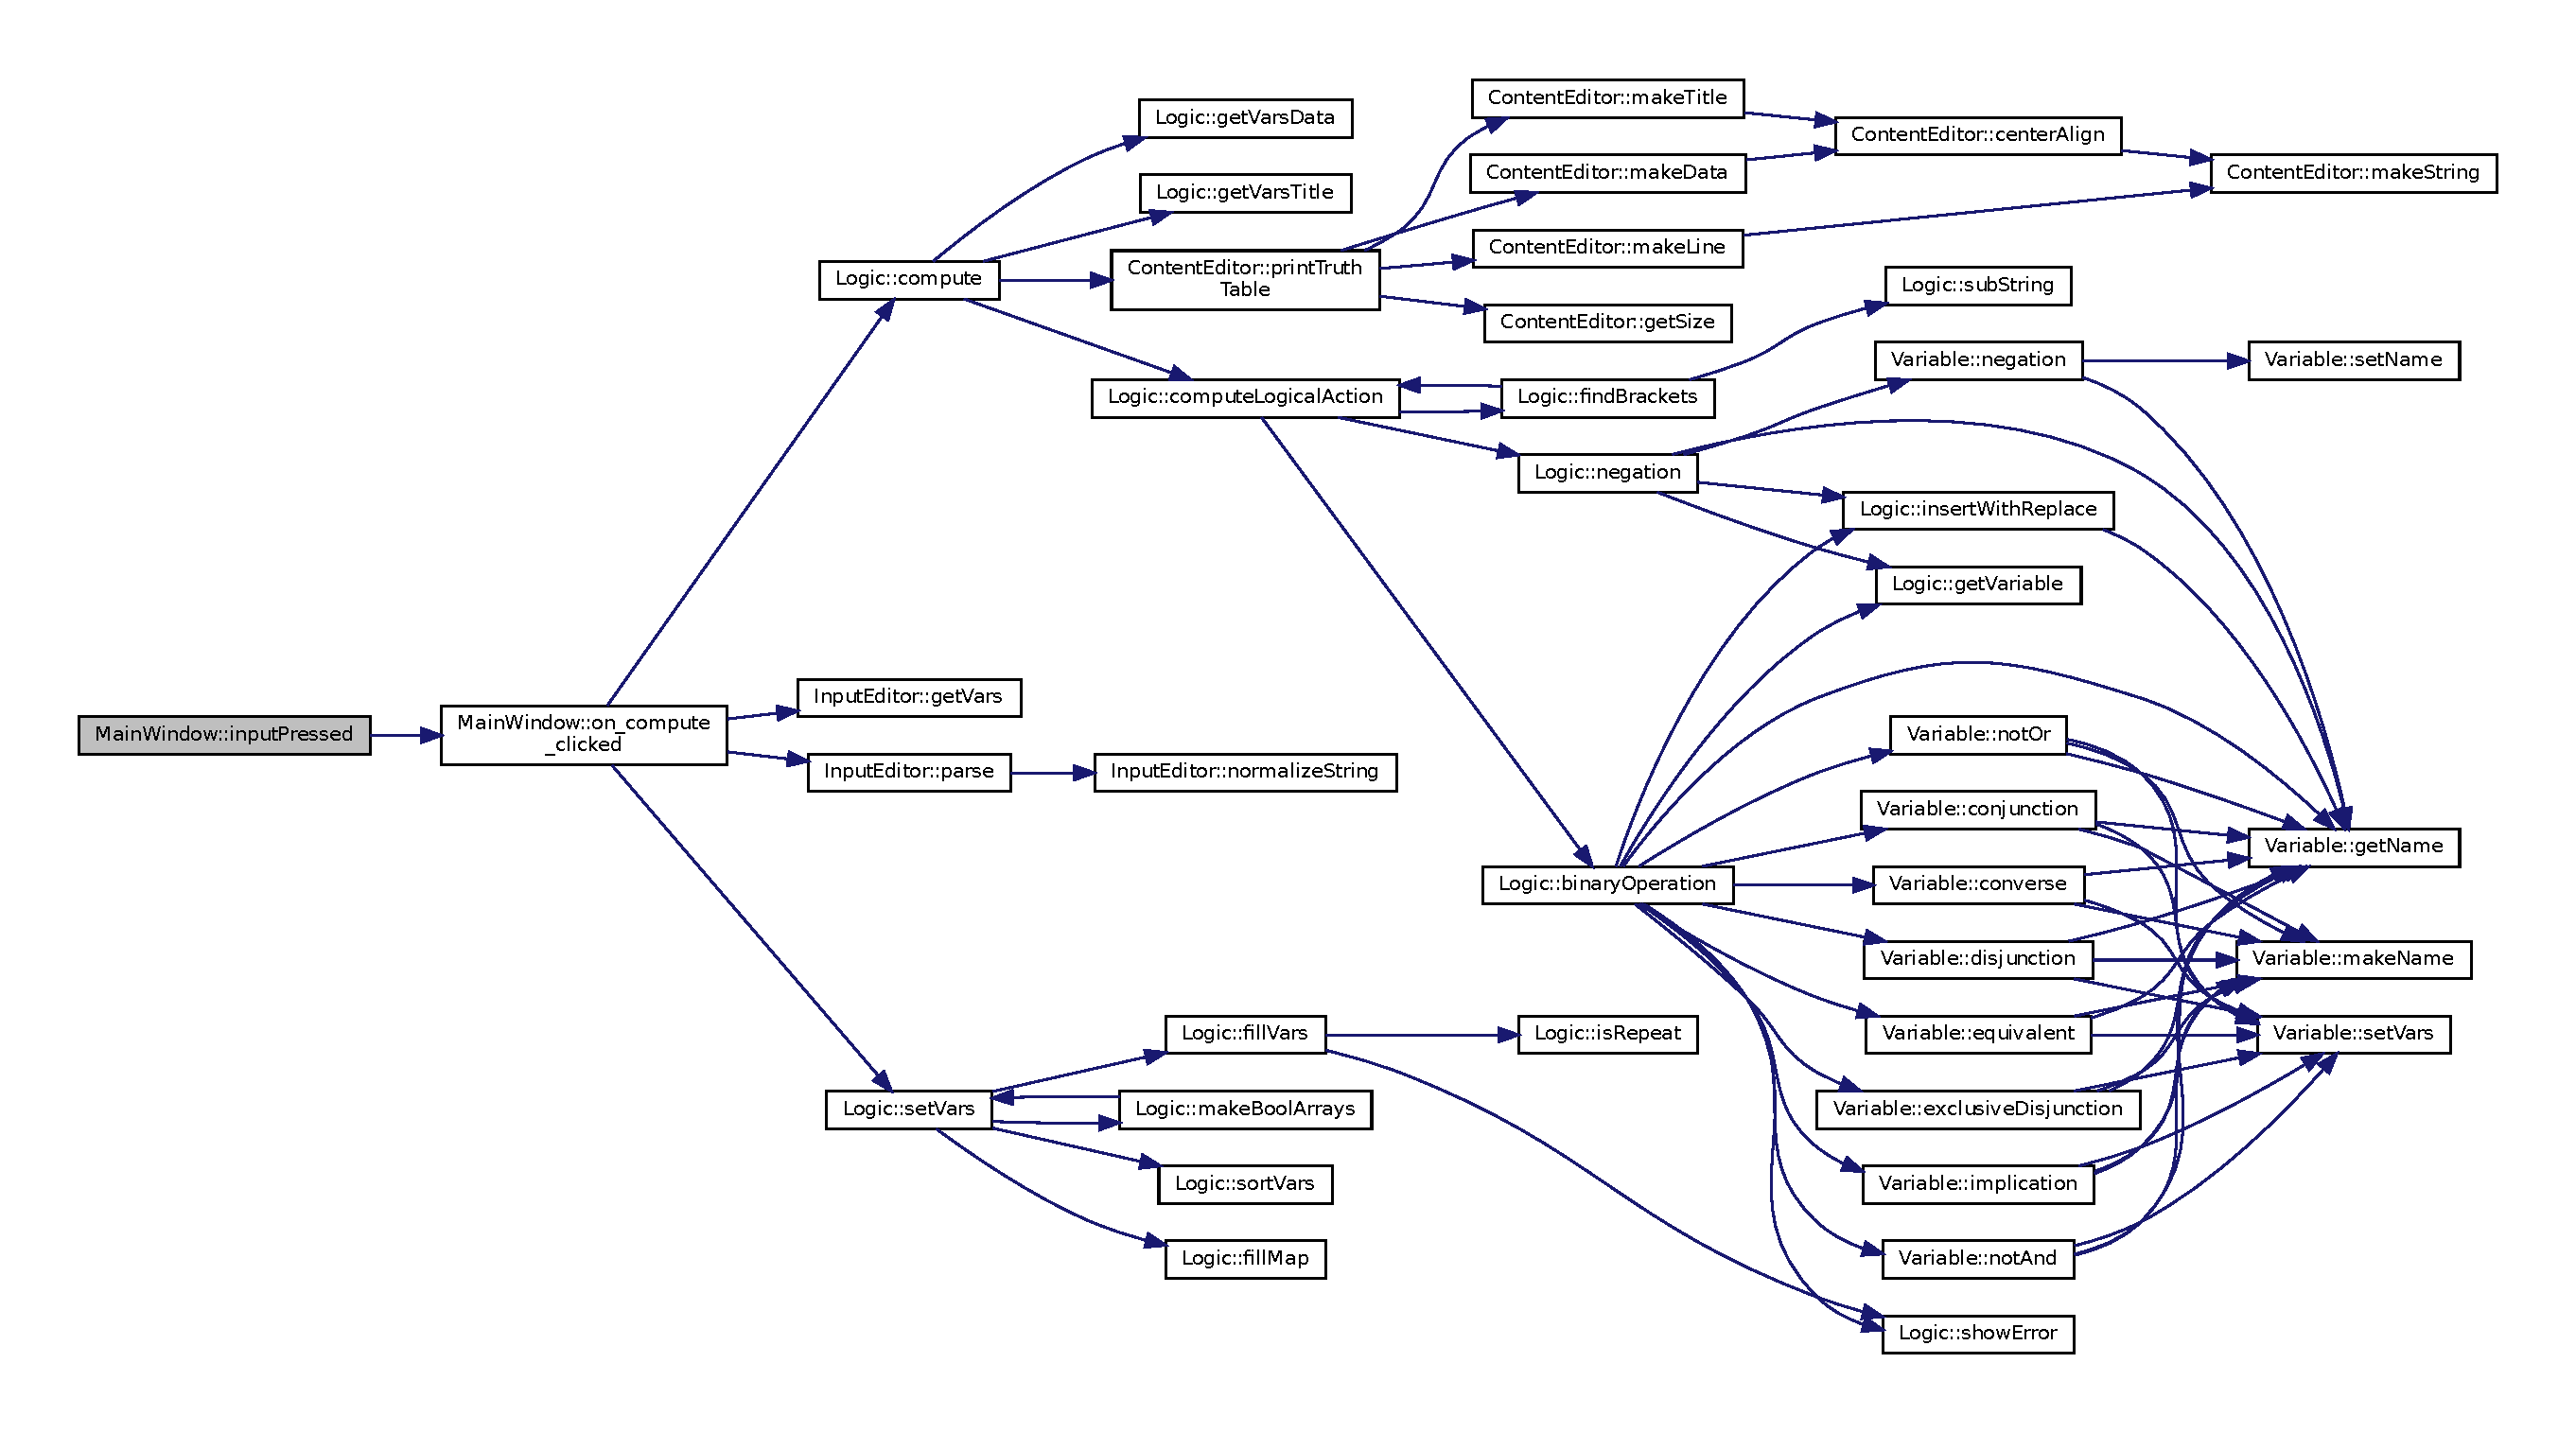
\includegraphics[width=350pt]{class_main_window_ad2b196b4c7680e1995c870863ee3cabe_cgraph}
\end{center}
\end{figure}
Граф вызова функции\+:\nopagebreak
\begin{figure}[H]
\begin{center}
\leavevmode
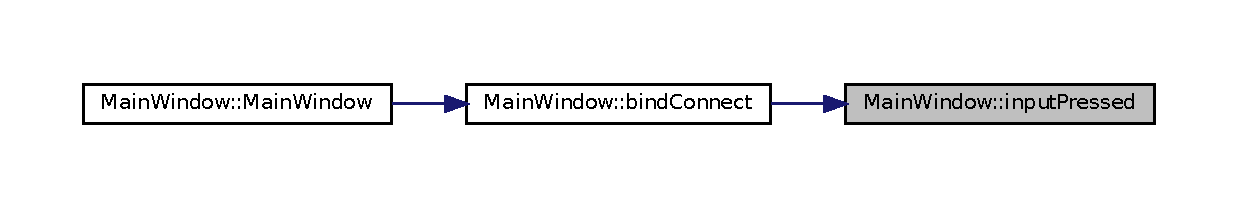
\includegraphics[width=350pt]{class_main_window_ad2b196b4c7680e1995c870863ee3cabe_icgraph}
\end{center}
\end{figure}
\mbox{\Hypertarget{class_main_window_a41bad26e9dbaae6c92d2a076797ef33c}\label{class_main_window_a41bad26e9dbaae6c92d2a076797ef33c}} 
\index{MainWindow@{MainWindow}!on\_compute\_clicked@{on\_compute\_clicked}}
\index{on\_compute\_clicked@{on\_compute\_clicked}!MainWindow@{MainWindow}}
\doxysubsubsection{\texorpdfstring{on\_compute\_clicked}{on\_compute\_clicked}}
{\footnotesize\ttfamily void Main\+Window\+::on\+\_\+compute\+\_\+clicked (\begin{DoxyParamCaption}{ }\end{DoxyParamCaption})\hspace{0.3cm}{\ttfamily [private]}, {\ttfamily [slot]}}



\mbox{\hyperlink{class_main_window_a41bad26e9dbaae6c92d2a076797ef33c}{Main\+Window\+::on\+\_\+compute\+\_\+clicked}} Обработчик нажатия на кнопку Вычислить 

Граф вызовов\+:\nopagebreak
\begin{figure}[H]
\begin{center}
\leavevmode
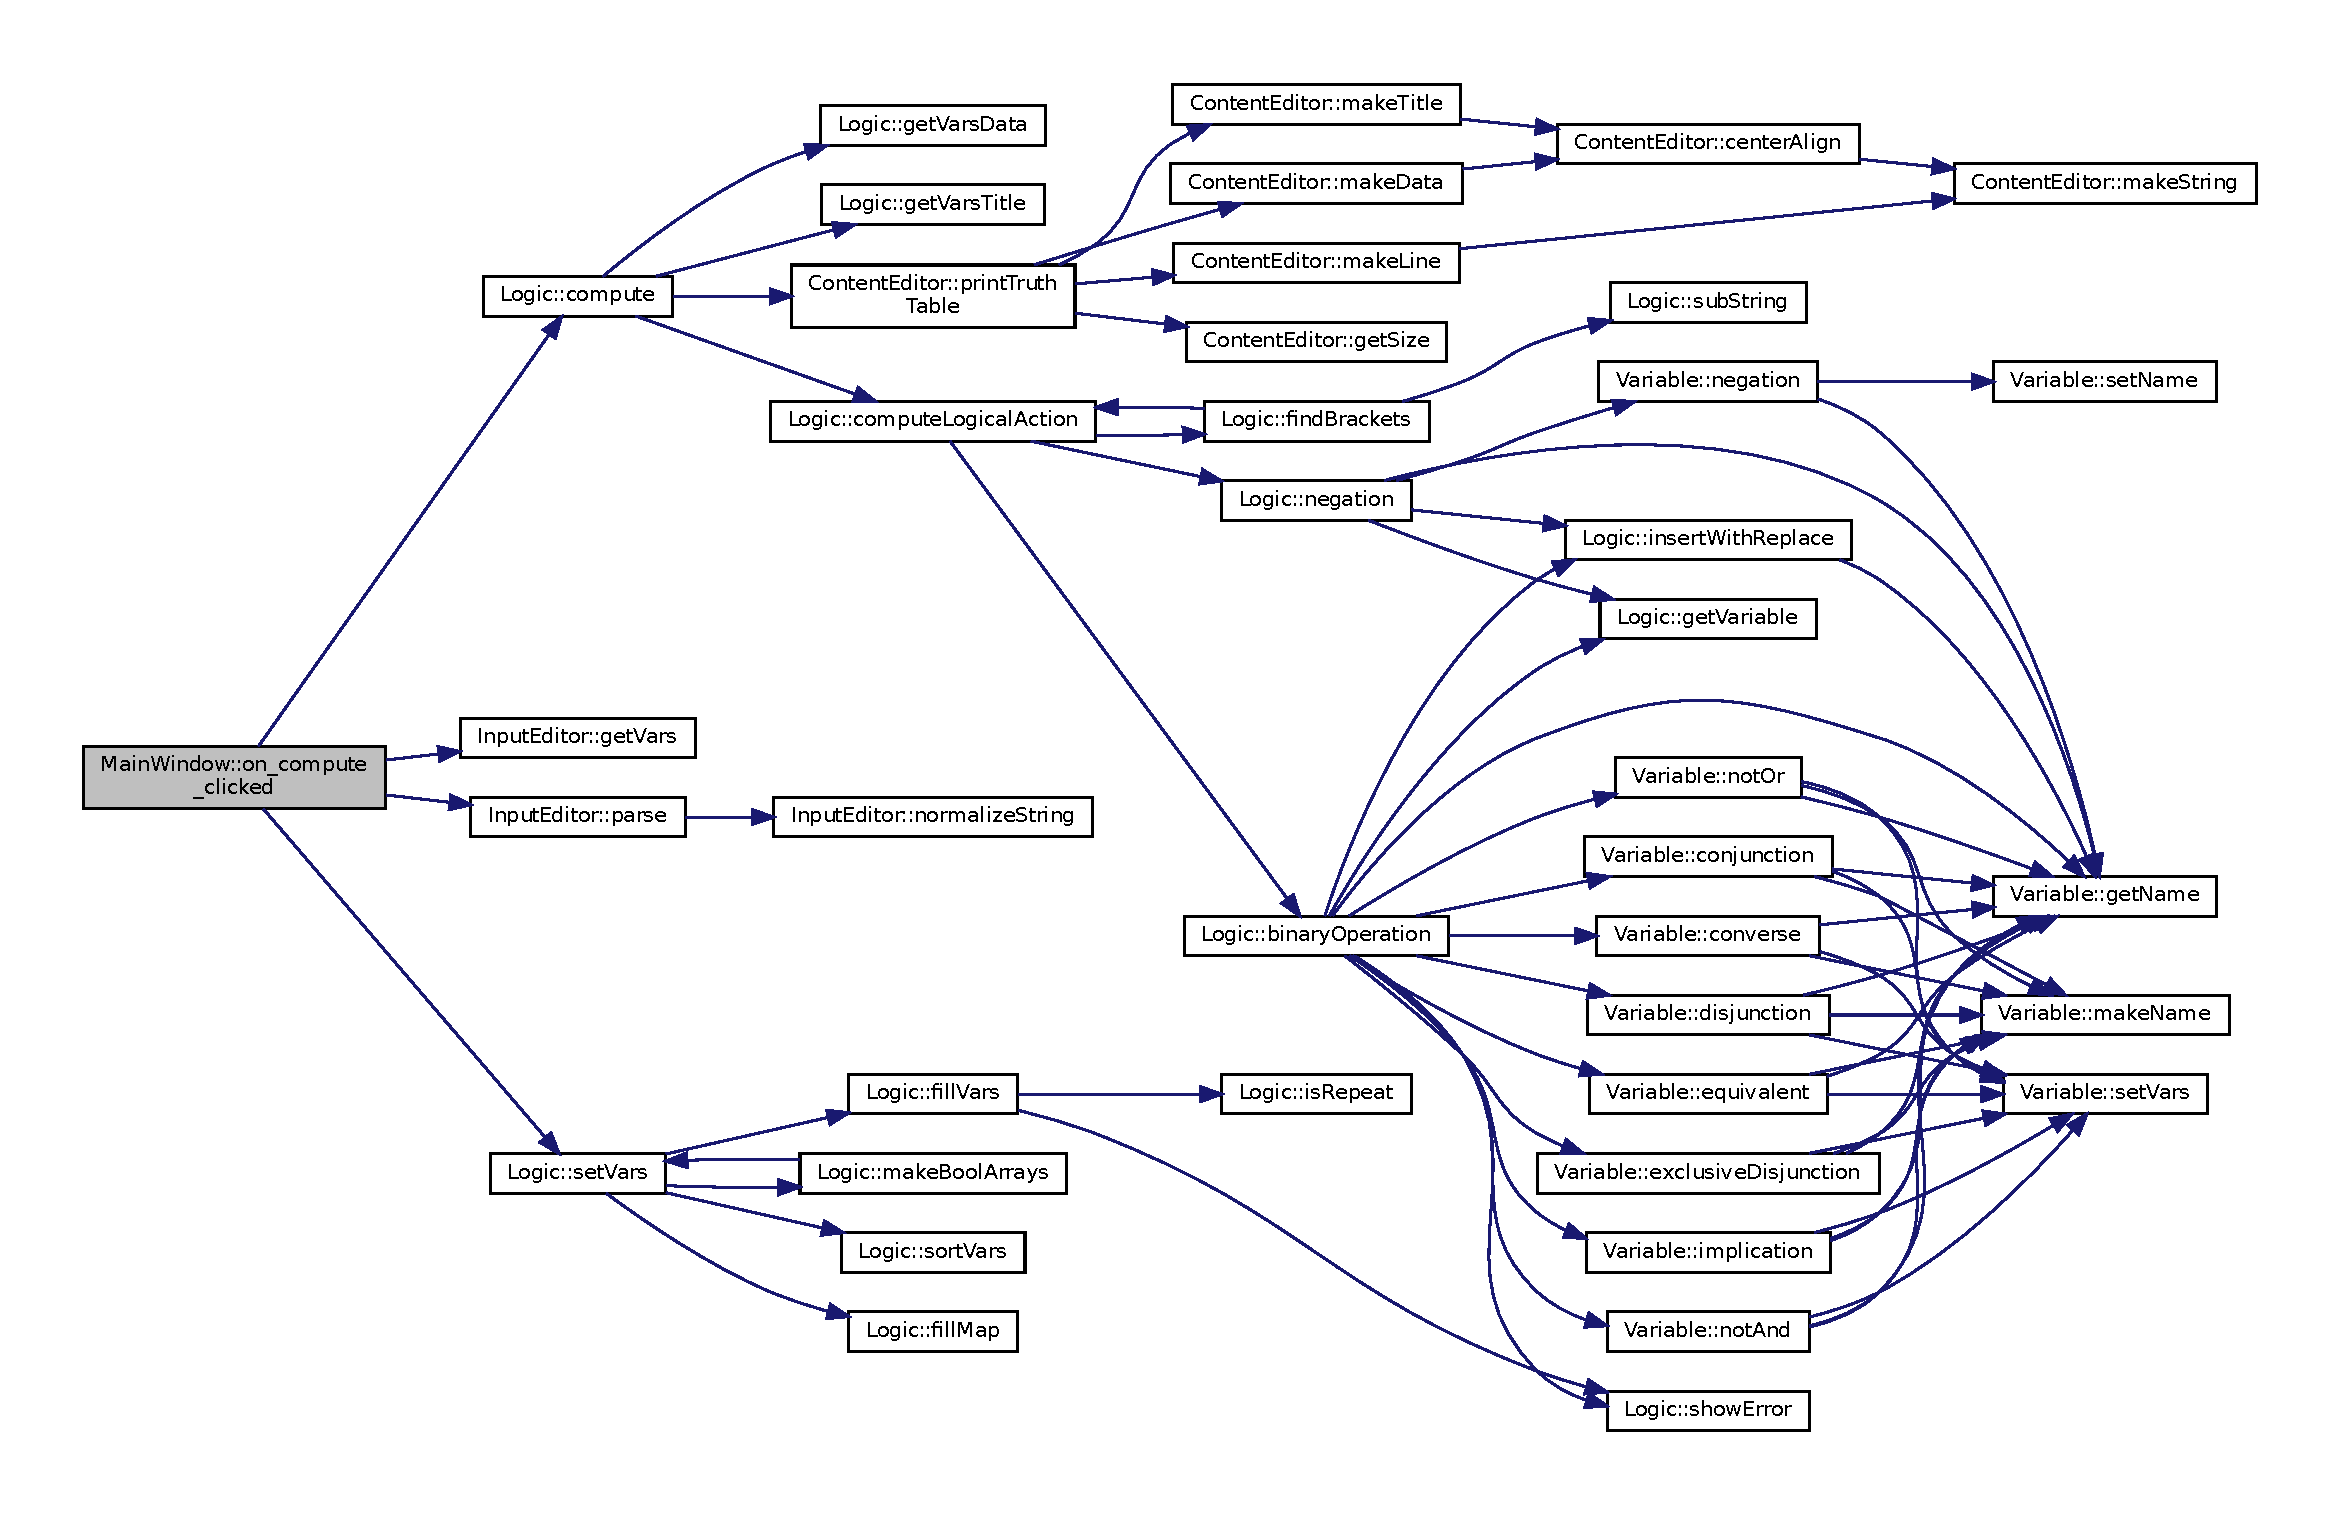
\includegraphics[width=350pt]{class_main_window_a41bad26e9dbaae6c92d2a076797ef33c_cgraph}
\end{center}
\end{figure}
Граф вызова функции\+:\nopagebreak
\begin{figure}[H]
\begin{center}
\leavevmode
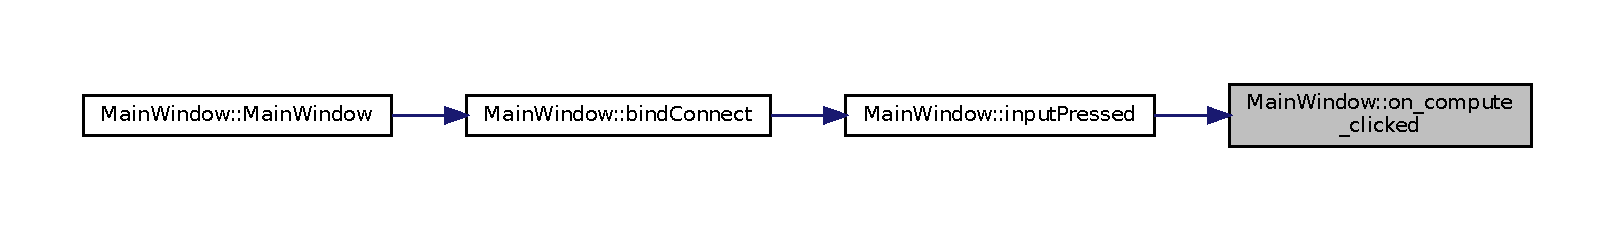
\includegraphics[width=350pt]{class_main_window_a41bad26e9dbaae6c92d2a076797ef33c_icgraph}
\end{center}
\end{figure}
\mbox{\Hypertarget{class_main_window_af483459fc458b993949c504e1e0d24af}\label{class_main_window_af483459fc458b993949c504e1e0d24af}} 
\index{MainWindow@{MainWindow}!on\_f4\_clicked@{on\_f4\_clicked}}
\index{on\_f4\_clicked@{on\_f4\_clicked}!MainWindow@{MainWindow}}
\doxysubsubsection{\texorpdfstring{on\_f4\_clicked}{on\_f4\_clicked}}
{\footnotesize\ttfamily void Main\+Window\+::on\+\_\+f4\+\_\+clicked (\begin{DoxyParamCaption}{ }\end{DoxyParamCaption})\hspace{0.3cm}{\ttfamily [private]}, {\ttfamily [slot]}}



\mbox{\hyperlink{class_main_window_af483459fc458b993949c504e1e0d24af}{Main\+Window\+::on\+\_\+f4\+\_\+clicked}} Обработчик для кнопки СДНФ 

Граф вызовов\+:\nopagebreak
\begin{figure}[H]
\begin{center}
\leavevmode
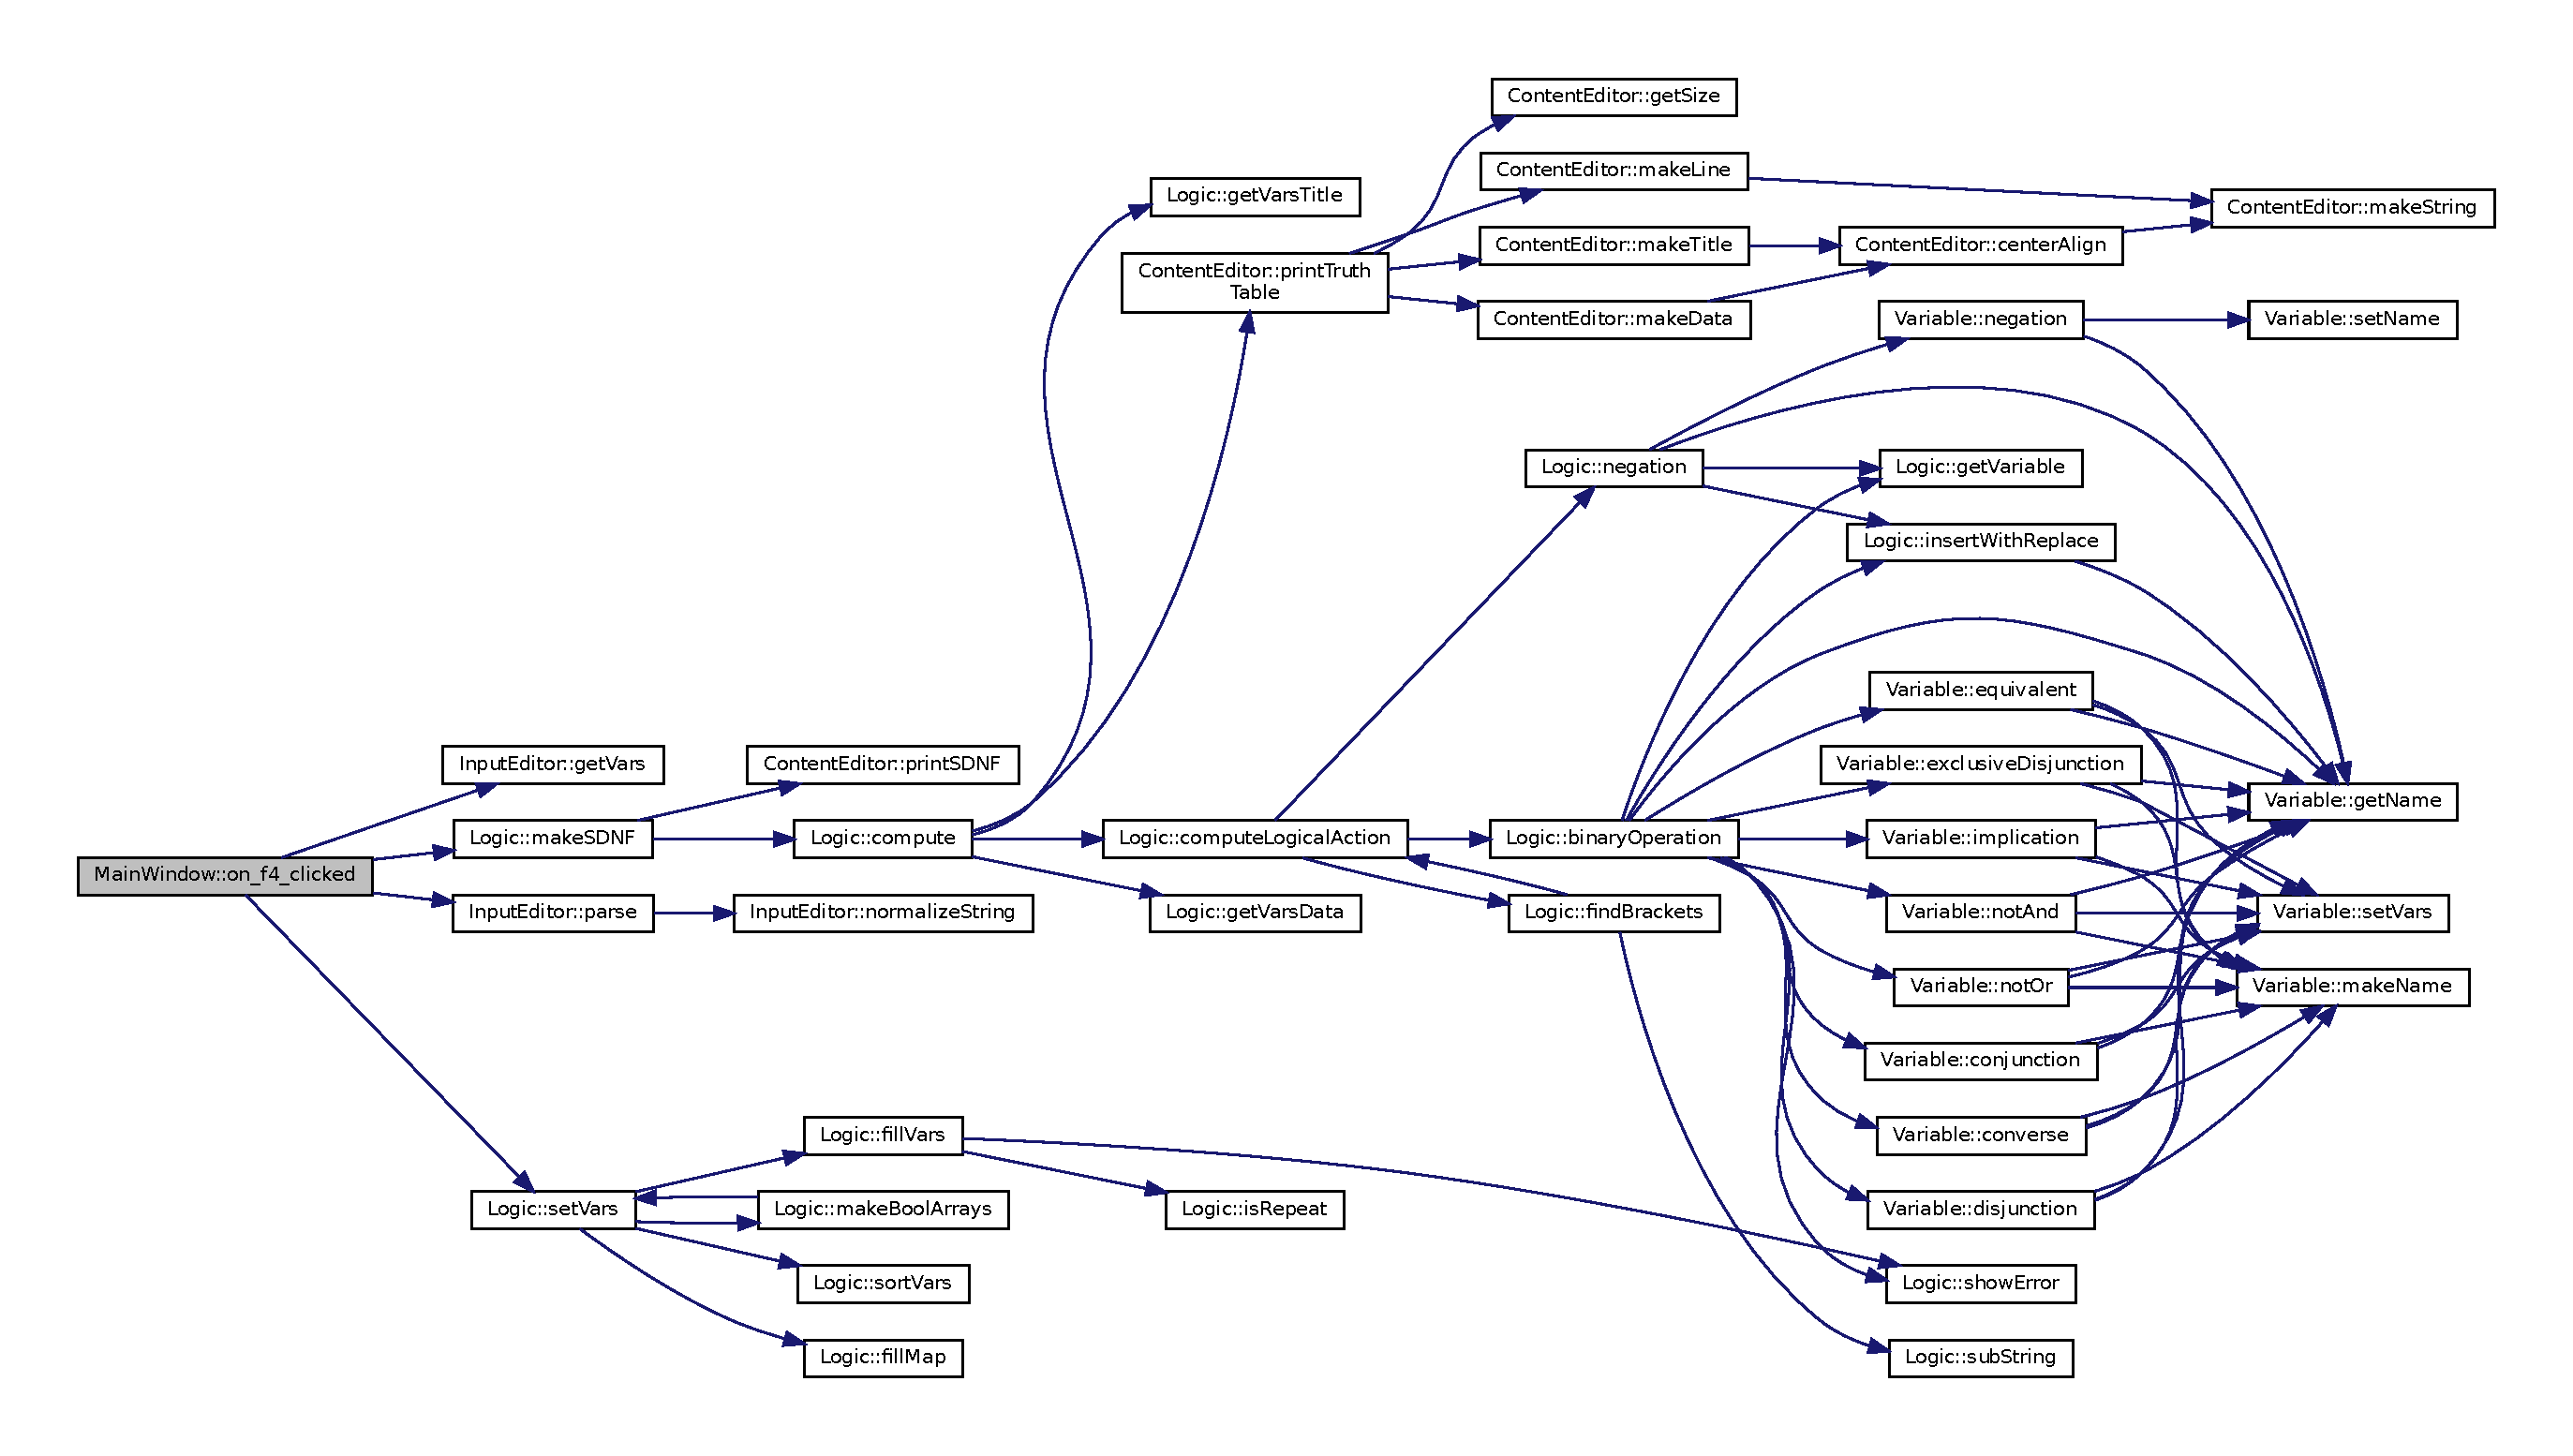
\includegraphics[width=350pt]{class_main_window_af483459fc458b993949c504e1e0d24af_cgraph}
\end{center}
\end{figure}
\mbox{\Hypertarget{class_main_window_a9823fb93ccc1255eb7c4a749478a74a6}\label{class_main_window_a9823fb93ccc1255eb7c4a749478a74a6}} 
\index{MainWindow@{MainWindow}!on\_f5\_clicked@{on\_f5\_clicked}}
\index{on\_f5\_clicked@{on\_f5\_clicked}!MainWindow@{MainWindow}}
\doxysubsubsection{\texorpdfstring{on\_f5\_clicked}{on\_f5\_clicked}}
{\footnotesize\ttfamily void Main\+Window\+::on\+\_\+f5\+\_\+clicked (\begin{DoxyParamCaption}{ }\end{DoxyParamCaption})\hspace{0.3cm}{\ttfamily [private]}, {\ttfamily [slot]}}



\mbox{\hyperlink{class_main_window_a9823fb93ccc1255eb7c4a749478a74a6}{Main\+Window\+::on\+\_\+f5\+\_\+clicked}} Обработчик для кнопки СКНФ 

Граф вызовов\+:\nopagebreak
\begin{figure}[H]
\begin{center}
\leavevmode
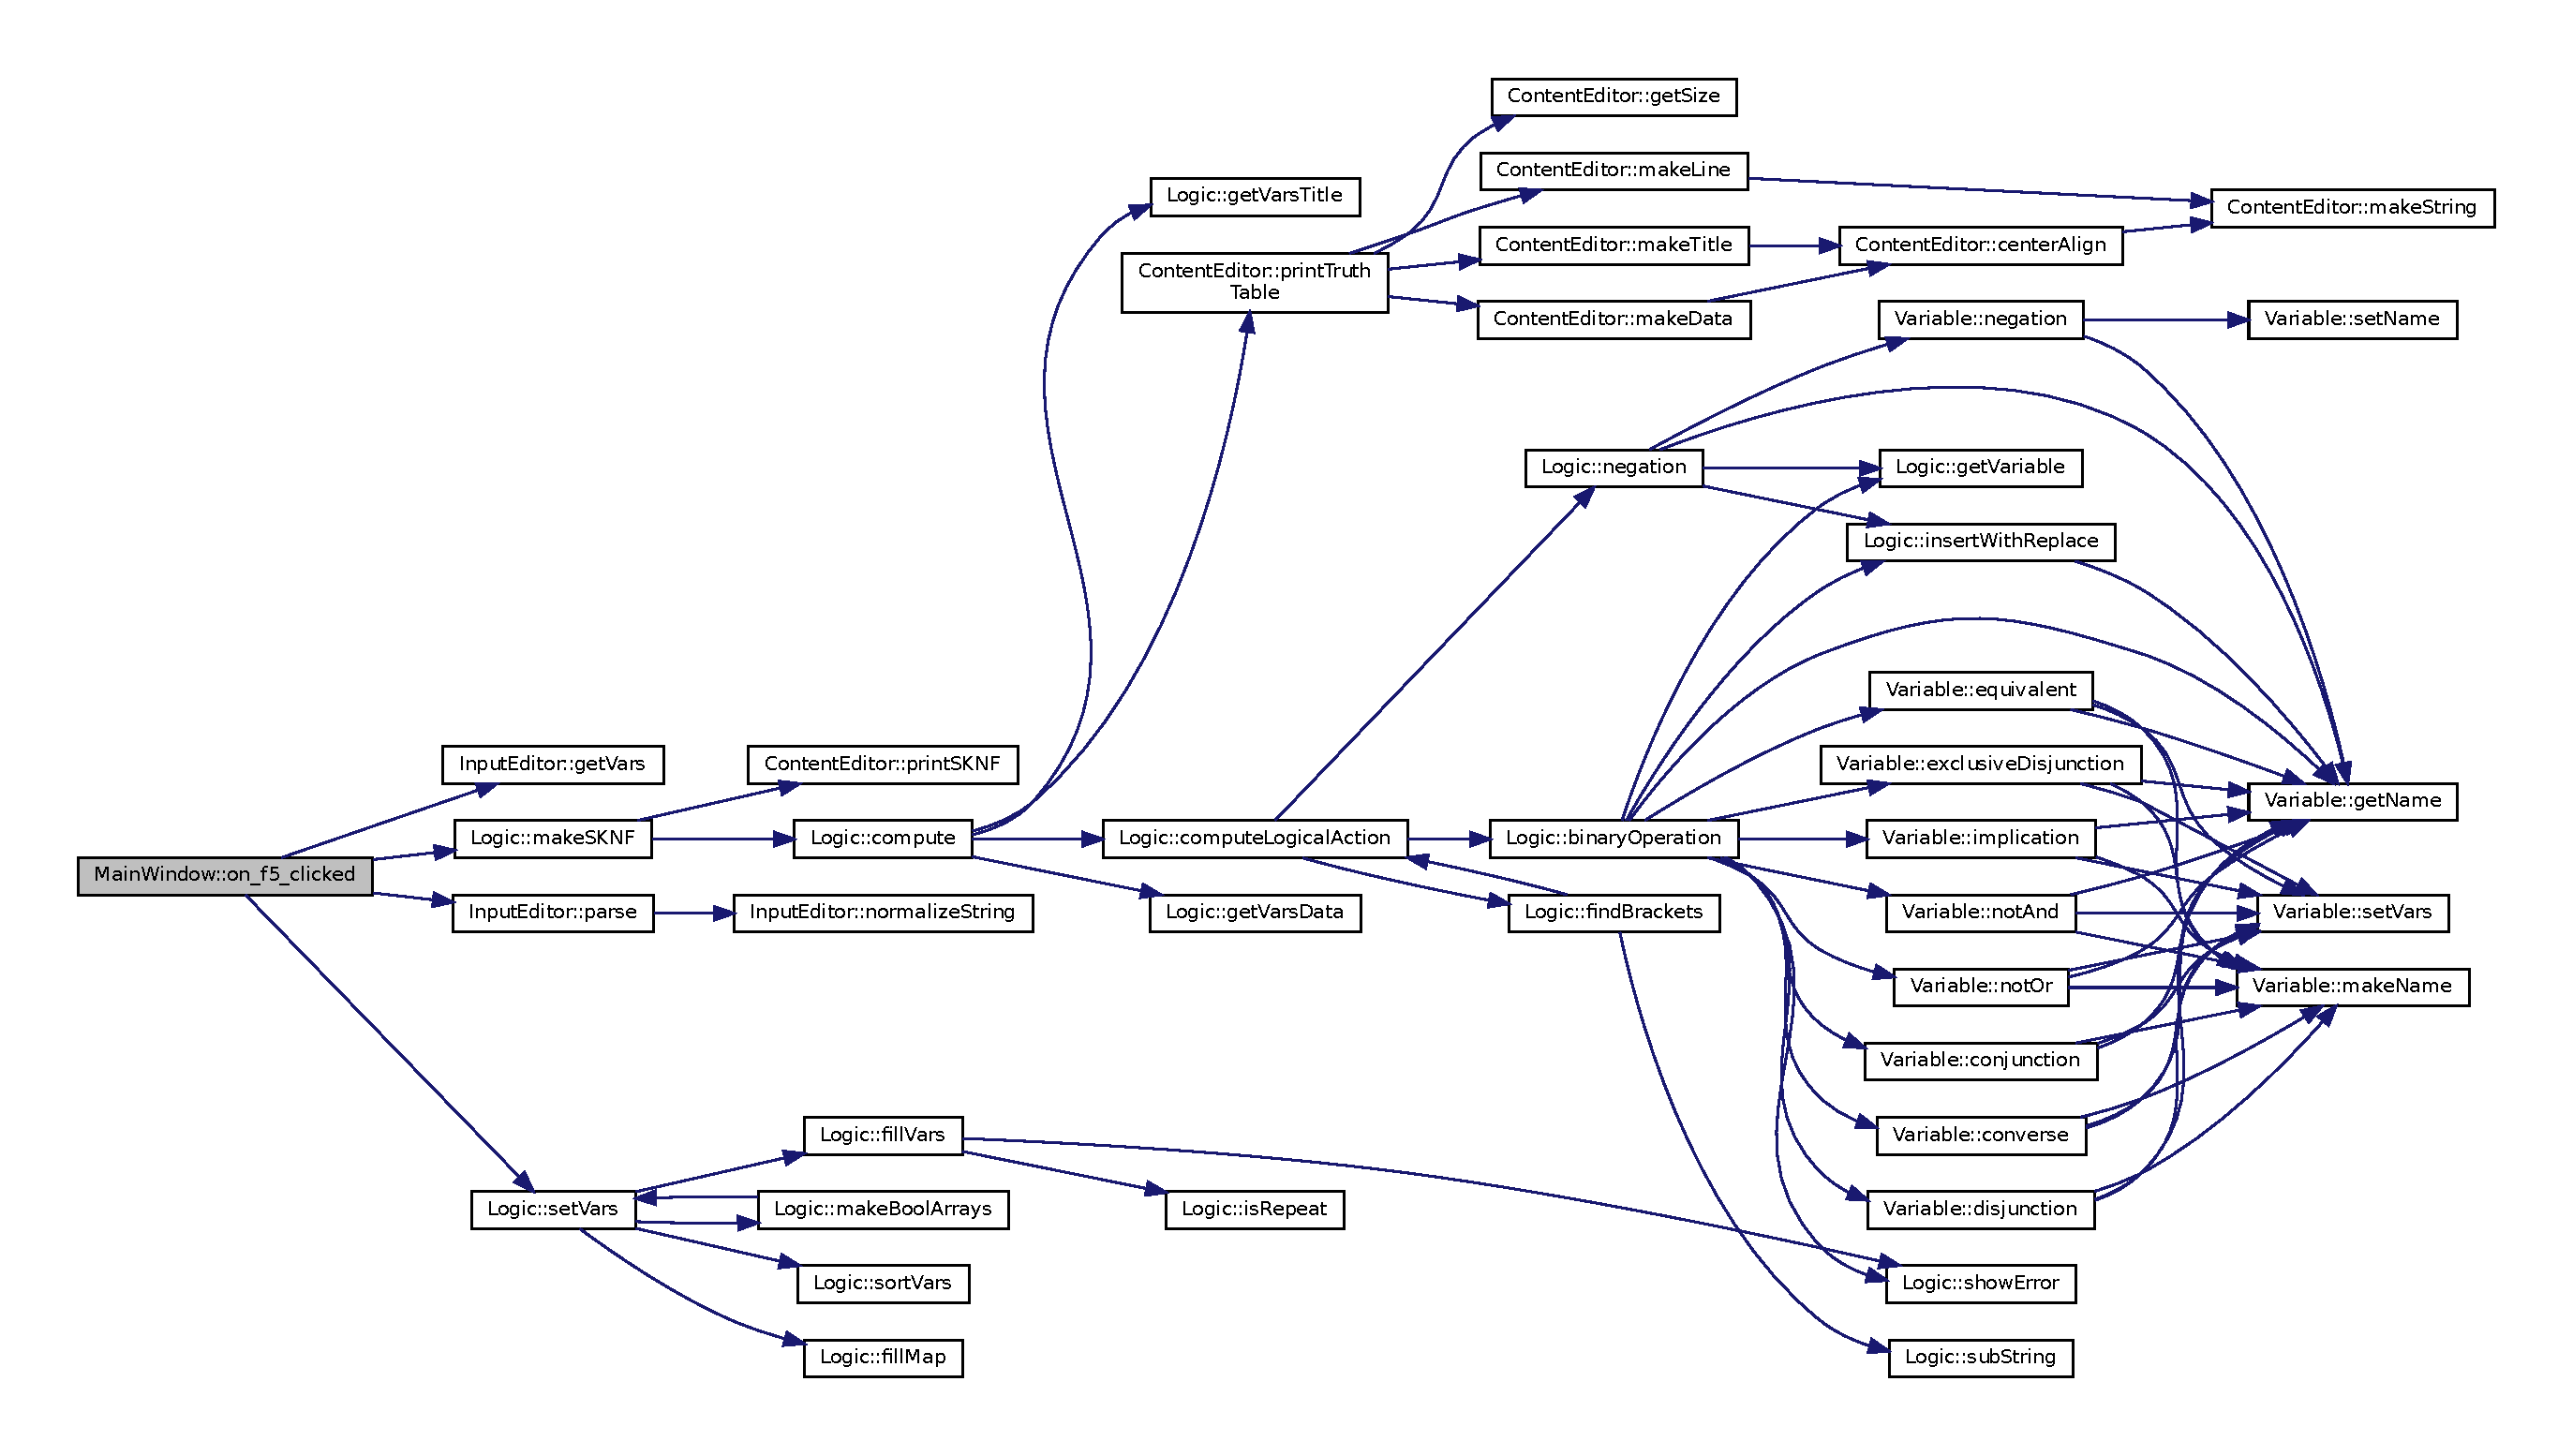
\includegraphics[width=350pt]{class_main_window_a9823fb93ccc1255eb7c4a749478a74a6_cgraph}
\end{center}
\end{figure}
\mbox{\Hypertarget{class_main_window_a35937dfc64e91849432cf75714cafcc7}\label{class_main_window_a35937dfc64e91849432cf75714cafcc7}} 
\index{MainWindow@{MainWindow}!onClicked@{onClicked}}
\index{onClicked@{onClicked}!MainWindow@{MainWindow}}
\doxysubsubsection{\texorpdfstring{onClicked}{onClicked}}
{\footnotesize\ttfamily void Main\+Window\+::on\+Clicked (\begin{DoxyParamCaption}{ }\end{DoxyParamCaption})\hspace{0.3cm}{\ttfamily [private]}, {\ttfamily [slot]}}



\mbox{\hyperlink{class_main_window_a35937dfc64e91849432cf75714cafcc7}{Main\+Window\+::on\+Clicked}} Обработчик на кнопки логических операций. Добавляет в поле ввода данных соответствующий символ 

Граф вызовов\+:\nopagebreak
\begin{figure}[H]
\begin{center}
\leavevmode
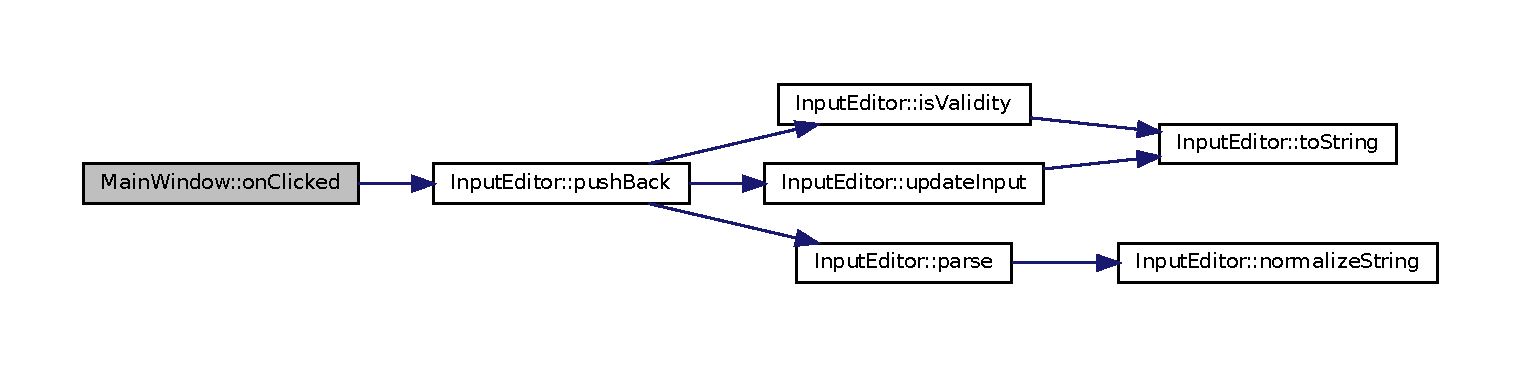
\includegraphics[width=350pt]{class_main_window_a35937dfc64e91849432cf75714cafcc7_cgraph}
\end{center}
\end{figure}
Граф вызова функции\+:\nopagebreak
\begin{figure}[H]
\begin{center}
\leavevmode
\includegraphics[width=350pt]{class_main_window_a35937dfc64e91849432cf75714cafcc7_icgraph}
\end{center}
\end{figure}


\doxysubsection{Данные класса}
\mbox{\Hypertarget{class_main_window_a44dcd3d3c75c90b005c644b26c58ac21}\label{class_main_window_a44dcd3d3c75c90b005c644b26c58ac21}} 
\index{MainWindow@{MainWindow}!ie\_@{ie\_}}
\index{ie\_@{ie\_}!MainWindow@{MainWindow}}
\doxysubsubsection{\texorpdfstring{ie\_}{ie\_}}
{\footnotesize\ttfamily \mbox{\hyperlink{class_input_editor}{Input\+Editor}}$\ast$ Main\+Window\+::ie\+\_\+\hspace{0.3cm}{\ttfamily [private]}}

\mbox{\Hypertarget{class_main_window_a2362702e2f4888ead84da68a75c595d7}\label{class_main_window_a2362702e2f4888ead84da68a75c595d7}} 
\index{MainWindow@{MainWindow}!logic\_@{logic\_}}
\index{logic\_@{logic\_}!MainWindow@{MainWindow}}
\doxysubsubsection{\texorpdfstring{logic\_}{logic\_}}
{\footnotesize\ttfamily \mbox{\hyperlink{class_logic}{Logic}}$\ast$ Main\+Window\+::logic\+\_\+\hspace{0.3cm}{\ttfamily [private]}}



отвечает за обработку данных, вводимых в поле ввода данных 

\mbox{\Hypertarget{class_main_window_a35466a70ed47252a0191168126a352a5}\label{class_main_window_a35466a70ed47252a0191168126a352a5}} 
\index{MainWindow@{MainWindow}!ui@{ui}}
\index{ui@{ui}!MainWindow@{MainWindow}}
\doxysubsubsection{\texorpdfstring{ui}{ui}}
{\footnotesize\ttfamily Ui\+::\+Main\+Window$\ast$ Main\+Window\+::ui}



Объявления и описания членов классов находятся в файлах\+:\begin{DoxyCompactItemize}
\item 
/home/mike/projects/logic\+\_\+calculator/\mbox{\hyperlink{mainwindow_8h}{mainwindow.\+h}}\item 
/home/mike/projects/logic\+\_\+calculator/\mbox{\hyperlink{mainwindow_8cpp}{mainwindow.\+cpp}}\end{DoxyCompactItemize}

\hypertarget{class_variable}{}\doxysection{Класс Variable}
\label{class_variable}\index{Variable@{Variable}}


\mbox{\hyperlink{class_variable}{Variable}} -\/ Класс логических переменных  




{\ttfamily \#include $<$variable.\+h$>$}

\doxysubsection*{Открытые члены}
\begin{DoxyCompactItemize}
\item 
\mbox{\hyperlink{class_variable_abef86be74e8dfb025fdeaf18048e9922}{Variable}} (const Q\+Char name)
\item 
\mbox{\hyperlink{class_variable_ae347cff8c66e1fb58b5fd90b9f19956a}{Variable}} (const Q\+String \&name)
\item 
\mbox{\hyperlink{class_variable_af3512a97c66e98c40a4aa69c9d65e22a}{Variable}} (const Q\+Char name, const Q\+List$<$ bool $>$ $\ast$vars)
\item 
\mbox{\hyperlink{class_variable_af55f1231f40b8fc1bb6fbca091a43c83}{Variable}} (Q\+Char name, int number\+Variables, int position\+Variable)
\item 
\mbox{\hyperlink{class_variable}{Variable}} \mbox{\hyperlink{class_variable_a3072441748b17a105aea1485911bb489}{conjunction}} (const \mbox{\hyperlink{class_variable}{Variable}} \&other) const
\begin{DoxyCompactList}\small\item\em \mbox{\hyperlink{class_variable_a3072441748b17a105aea1485911bb489}{Variable\+::conjunction}} Конъюнкция \end{DoxyCompactList}\item 
\mbox{\hyperlink{class_variable}{Variable}} \mbox{\hyperlink{class_variable_a2e4849eea01ce6e2ec9ba143164e7d57}{disjunction}} (const \mbox{\hyperlink{class_variable}{Variable}} \&other) const
\begin{DoxyCompactList}\small\item\em \mbox{\hyperlink{class_variable_a2e4849eea01ce6e2ec9ba143164e7d57}{Variable\+::disjunction}} Дизъюнкция \end{DoxyCompactList}\item 
\mbox{\hyperlink{class_variable}{Variable}} \mbox{\hyperlink{class_variable_a82a20d70ad58a132b487a7bc822b47d1}{implication}} (const \mbox{\hyperlink{class_variable}{Variable}} \&other) const
\begin{DoxyCompactList}\small\item\em \mbox{\hyperlink{class_variable_a82a20d70ad58a132b487a7bc822b47d1}{Variable\+::implication}} Импликация \end{DoxyCompactList}\item 
\mbox{\hyperlink{class_variable}{Variable}} \mbox{\hyperlink{class_variable_adb62912a5e9433289191879e6bb7d580}{converse}} (const \mbox{\hyperlink{class_variable}{Variable}} \&other) const
\begin{DoxyCompactList}\small\item\em \mbox{\hyperlink{class_variable_adb62912a5e9433289191879e6bb7d580}{Variable\+::converse}} Обратная импликация \end{DoxyCompactList}\item 
\mbox{\hyperlink{class_variable}{Variable}} \mbox{\hyperlink{class_variable_a5b1b5220dae873cc4bf6d0700eba703e}{not\+And}} (const \mbox{\hyperlink{class_variable}{Variable}} \&other) const
\begin{DoxyCompactList}\small\item\em \mbox{\hyperlink{class_variable_a5b1b5220dae873cc4bf6d0700eba703e}{Variable\+::not\+And}} Штрих Шеффера \end{DoxyCompactList}\item 
\mbox{\hyperlink{class_variable}{Variable}} \mbox{\hyperlink{class_variable_aa71e11142a257fa6676257843879148c}{not\+Or}} (const \mbox{\hyperlink{class_variable}{Variable}} \&other) const
\begin{DoxyCompactList}\small\item\em \mbox{\hyperlink{class_variable_aa71e11142a257fa6676257843879148c}{Variable\+::not\+Or}} Стрелка Пирса \end{DoxyCompactList}\item 
\mbox{\hyperlink{class_variable}{Variable}} \mbox{\hyperlink{class_variable_a768fb534653ecc15e72f5d1201963705}{exclusive\+Disjunction}} (const \mbox{\hyperlink{class_variable}{Variable}} \&other) const
\begin{DoxyCompactList}\small\item\em \mbox{\hyperlink{class_variable_a768fb534653ecc15e72f5d1201963705}{Variable\+::exclusive\+Disjunction}} Исключающее ИЛИ \end{DoxyCompactList}\item 
\mbox{\hyperlink{class_variable}{Variable}} \mbox{\hyperlink{class_variable_a104b427ab0f43e9eb24f049ec6b524b0}{equivalent}} (const \mbox{\hyperlink{class_variable}{Variable}} \&other) const
\begin{DoxyCompactList}\small\item\em \mbox{\hyperlink{class_variable_a104b427ab0f43e9eb24f049ec6b524b0}{Variable\+::equivalent}} Эквиваленция \end{DoxyCompactList}\item 
\mbox{\hyperlink{class_variable}{Variable}} \mbox{\hyperlink{class_variable_a7f2a3b1b8540781703f5435253171978}{negation}} ()
\begin{DoxyCompactList}\small\item\em \mbox{\hyperlink{class_variable_a7f2a3b1b8540781703f5435253171978}{Variable\+::negation}} Отрицание самой переменной \end{DoxyCompactList}\item 
void \mbox{\hyperlink{class_variable_ab58f8291d67e633fd1ad76148fad9e1a}{set\+Name}} (const Q\+String \&name)
\begin{DoxyCompactList}\small\item\em \mbox{\hyperlink{class_variable_ab58f8291d67e633fd1ad76148fad9e1a}{Variable\+::set\+Name}} Задает имя \end{DoxyCompactList}\item 
void \mbox{\hyperlink{class_variable_ae6ac554c0382b43f9a3e37c6382d4471}{set\+Vars}} (const Q\+List$<$ bool $>$ \&vars)
\begin{DoxyCompactList}\small\item\em \mbox{\hyperlink{class_variable_ae6ac554c0382b43f9a3e37c6382d4471}{Variable\+::set\+Vars}} Задает принимаемые значения \end{DoxyCompactList}\item 
void \mbox{\hyperlink{class_variable_a1f2f14a77dc0dbe91e6bd285afa67fc4}{set\+Vars}} (const int index, const int size)
\begin{DoxyCompactList}\small\item\em \mbox{\hyperlink{class_variable_ae6ac554c0382b43f9a3e37c6382d4471}{Variable\+::set\+Vars}} Генерирует значения \end{DoxyCompactList}\item 
Q\+String \mbox{\hyperlink{class_variable_a7e2bd08aff707fb67d67ce1914e9bb48}{get\+Name}} () const
\begin{DoxyCompactList}\small\item\em \mbox{\hyperlink{class_variable_a7e2bd08aff707fb67d67ce1914e9bb48}{Variable\+::get\+Name}} Отдает название \end{DoxyCompactList}\item 
Q\+List$<$ bool $>$ \mbox{\hyperlink{class_variable_a43a45b7c410b176f3240ac1630495c8d}{get\+Vars}} () const
\begin{DoxyCompactList}\small\item\em \mbox{\hyperlink{class_variable_a43a45b7c410b176f3240ac1630495c8d}{Variable\+::get\+Vars}} Отдает значения переменной \end{DoxyCompactList}\item 
bool \mbox{\hyperlink{class_variable_a94991de2c5fd8fd5a66b74f726f0c645}{operator$>$}} (const \mbox{\hyperlink{class_variable}{Variable}} \&other)
\begin{DoxyCompactList}\small\item\em \mbox{\hyperlink{class_variable_a94991de2c5fd8fd5a66b74f726f0c645}{Variable\+::operator $>$}} оператор больше \end{DoxyCompactList}\item 
bool \mbox{\hyperlink{class_variable_ac0aa608ee2a38525351a6a5d902a466f}{operator$<$}} (const \mbox{\hyperlink{class_variable}{Variable}} \&other)
\begin{DoxyCompactList}\small\item\em \mbox{\hyperlink{class_variable_ac0aa608ee2a38525351a6a5d902a466f}{Variable\+::operator $<$}} оператор меньше \end{DoxyCompactList}\end{DoxyCompactItemize}
\doxysubsection*{Закрытые члены}
\begin{DoxyCompactItemize}
\item 
void \mbox{\hyperlink{class_variable_a9ab358fc363aa26fb83bc78297c3339a}{debug\+Vars}} ()
\item 
int \mbox{\hyperlink{class_variable_a53fda71f7c848f9b50fbb513fdabdeca}{pow2}} (const int power) const
\begin{DoxyCompactList}\small\item\em \mbox{\hyperlink{class_variable_a53fda71f7c848f9b50fbb513fdabdeca}{Variable\+::pow2}} Возвращает степень числа два \end{DoxyCompactList}\item 
Q\+String \mbox{\hyperlink{class_variable_a3bd6766c017a7ec86ecd18ed12780da6}{make\+Name}} (const Q\+String \&first, const Q\+String \&operation, const Q\+String \&second) const
\begin{DoxyCompactList}\small\item\em \mbox{\hyperlink{class_variable_a3bd6766c017a7ec86ecd18ed12780da6}{Variable\+::make\+Name}} Создает строку из двух названий переменных и операции между ними \end{DoxyCompactList}\end{DoxyCompactItemize}
\doxysubsection*{Закрытые данные}
\begin{DoxyCompactItemize}
\item 
Q\+String \mbox{\hyperlink{class_variable_a07cdd3799f013336744818ac8adb2dcc}{name\+\_\+}}
\item 
Q\+List$<$ bool $>$ \mbox{\hyperlink{class_variable_abdcbd198a2a06b3c973c11856beaf1d5}{vars\+\_\+}}
\begin{DoxyCompactList}\small\item\em Имя логической переменной \end{DoxyCompactList}\end{DoxyCompactItemize}


\doxysubsection{Подробное описание}
\mbox{\hyperlink{class_variable}{Variable}} -\/ Класс логических переменных 

\doxysubsection{Конструктор(ы)}
\mbox{\Hypertarget{class_variable_abef86be74e8dfb025fdeaf18048e9922}\label{class_variable_abef86be74e8dfb025fdeaf18048e9922}} 
\index{Variable@{Variable}!Variable@{Variable}}
\index{Variable@{Variable}!Variable@{Variable}}
\doxysubsubsection{\texorpdfstring{Variable()}{Variable()}\hspace{0.1cm}{\footnotesize\ttfamily [1/4]}}
{\footnotesize\ttfamily Variable\+::\+Variable (\begin{DoxyParamCaption}\item[{const Q\+Char}]{name }\end{DoxyParamCaption})}

Граф вызовов\+:\nopagebreak
\begin{figure}[H]
\begin{center}
\leavevmode
\includegraphics[width=325pt]{class_variable_abef86be74e8dfb025fdeaf18048e9922_cgraph}
\end{center}
\end{figure}
\mbox{\Hypertarget{class_variable_ae347cff8c66e1fb58b5fd90b9f19956a}\label{class_variable_ae347cff8c66e1fb58b5fd90b9f19956a}} 
\index{Variable@{Variable}!Variable@{Variable}}
\index{Variable@{Variable}!Variable@{Variable}}
\doxysubsubsection{\texorpdfstring{Variable()}{Variable()}\hspace{0.1cm}{\footnotesize\ttfamily [2/4]}}
{\footnotesize\ttfamily Variable\+::\+Variable (\begin{DoxyParamCaption}\item[{const Q\+String \&}]{name }\end{DoxyParamCaption})}

Граф вызовов\+:\nopagebreak
\begin{figure}[H]
\begin{center}
\leavevmode
\includegraphics[width=325pt]{class_variable_ae347cff8c66e1fb58b5fd90b9f19956a_cgraph}
\end{center}
\end{figure}
\mbox{\Hypertarget{class_variable_af3512a97c66e98c40a4aa69c9d65e22a}\label{class_variable_af3512a97c66e98c40a4aa69c9d65e22a}} 
\index{Variable@{Variable}!Variable@{Variable}}
\index{Variable@{Variable}!Variable@{Variable}}
\doxysubsubsection{\texorpdfstring{Variable()}{Variable()}\hspace{0.1cm}{\footnotesize\ttfamily [3/4]}}
{\footnotesize\ttfamily Variable\+::\+Variable (\begin{DoxyParamCaption}\item[{const Q\+Char}]{name,  }\item[{const Q\+List$<$ bool $>$ $\ast$}]{vars }\end{DoxyParamCaption})}

Граф вызовов\+:\nopagebreak
\begin{figure}[H]
\begin{center}
\leavevmode
\includegraphics[width=325pt]{class_variable_af3512a97c66e98c40a4aa69c9d65e22a_cgraph}
\end{center}
\end{figure}
\mbox{\Hypertarget{class_variable_af55f1231f40b8fc1bb6fbca091a43c83}\label{class_variable_af55f1231f40b8fc1bb6fbca091a43c83}} 
\index{Variable@{Variable}!Variable@{Variable}}
\index{Variable@{Variable}!Variable@{Variable}}
\doxysubsubsection{\texorpdfstring{Variable()}{Variable()}\hspace{0.1cm}{\footnotesize\ttfamily [4/4]}}
{\footnotesize\ttfamily Variable\+::\+Variable (\begin{DoxyParamCaption}\item[{Q\+Char}]{name,  }\item[{int}]{number\+Variables,  }\item[{int}]{position\+Variable }\end{DoxyParamCaption})}

Граф вызовов\+:\nopagebreak
\begin{figure}[H]
\begin{center}
\leavevmode
\includegraphics[width=325pt]{class_variable_af55f1231f40b8fc1bb6fbca091a43c83_cgraph}
\end{center}
\end{figure}


\doxysubsection{Методы}
\mbox{\Hypertarget{class_variable_a3072441748b17a105aea1485911bb489}\label{class_variable_a3072441748b17a105aea1485911bb489}} 
\index{Variable@{Variable}!conjunction@{conjunction}}
\index{conjunction@{conjunction}!Variable@{Variable}}
\doxysubsubsection{\texorpdfstring{conjunction()}{conjunction()}}
{\footnotesize\ttfamily \mbox{\hyperlink{class_variable}{Variable}} Variable\+::conjunction (\begin{DoxyParamCaption}\item[{const \mbox{\hyperlink{class_variable}{Variable}} \&}]{other }\end{DoxyParamCaption}) const}



\mbox{\hyperlink{class_variable_a3072441748b17a105aea1485911bb489}{Variable\+::conjunction}} Конъюнкция 


\begin{DoxyParams}{Аргументы}
{\em other} & с данной переменной \\
\hline
\end{DoxyParams}
\begin{DoxyReturn}{Возвращает}
Получившееся значение 
\end{DoxyReturn}
Граф вызовов\+:\nopagebreak
\begin{figure}[H]
\begin{center}
\leavevmode
\includegraphics[width=350pt]{class_variable_a3072441748b17a105aea1485911bb489_cgraph}
\end{center}
\end{figure}
Граф вызова функции\+:\nopagebreak
\begin{figure}[H]
\begin{center}
\leavevmode
\includegraphics[width=350pt]{class_variable_a3072441748b17a105aea1485911bb489_icgraph}
\end{center}
\end{figure}
\mbox{\Hypertarget{class_variable_adb62912a5e9433289191879e6bb7d580}\label{class_variable_adb62912a5e9433289191879e6bb7d580}} 
\index{Variable@{Variable}!converse@{converse}}
\index{converse@{converse}!Variable@{Variable}}
\doxysubsubsection{\texorpdfstring{converse()}{converse()}}
{\footnotesize\ttfamily \mbox{\hyperlink{class_variable}{Variable}} Variable\+::converse (\begin{DoxyParamCaption}\item[{const \mbox{\hyperlink{class_variable}{Variable}} \&}]{other }\end{DoxyParamCaption}) const}



\mbox{\hyperlink{class_variable_adb62912a5e9433289191879e6bb7d580}{Variable\+::converse}} Обратная импликация 


\begin{DoxyParams}{Аргументы}
{\em other} & с данной переменной \\
\hline
\end{DoxyParams}
\begin{DoxyReturn}{Возвращает}
Получившееся значение 
\end{DoxyReturn}
Граф вызовов\+:\nopagebreak
\begin{figure}[H]
\begin{center}
\leavevmode
\includegraphics[width=342pt]{class_variable_adb62912a5e9433289191879e6bb7d580_cgraph}
\end{center}
\end{figure}
Граф вызова функции\+:\nopagebreak
\begin{figure}[H]
\begin{center}
\leavevmode
\includegraphics[width=350pt]{class_variable_adb62912a5e9433289191879e6bb7d580_icgraph}
\end{center}
\end{figure}
\mbox{\Hypertarget{class_variable_a9ab358fc363aa26fb83bc78297c3339a}\label{class_variable_a9ab358fc363aa26fb83bc78297c3339a}} 
\index{Variable@{Variable}!debugVars@{debugVars}}
\index{debugVars@{debugVars}!Variable@{Variable}}
\doxysubsubsection{\texorpdfstring{debugVars()}{debugVars()}}
{\footnotesize\ttfamily void Variable\+::debug\+Vars (\begin{DoxyParamCaption}{ }\end{DoxyParamCaption})\hspace{0.3cm}{\ttfamily [private]}}

\mbox{\Hypertarget{class_variable_a2e4849eea01ce6e2ec9ba143164e7d57}\label{class_variable_a2e4849eea01ce6e2ec9ba143164e7d57}} 
\index{Variable@{Variable}!disjunction@{disjunction}}
\index{disjunction@{disjunction}!Variable@{Variable}}
\doxysubsubsection{\texorpdfstring{disjunction()}{disjunction()}}
{\footnotesize\ttfamily \mbox{\hyperlink{class_variable}{Variable}} Variable\+::disjunction (\begin{DoxyParamCaption}\item[{const \mbox{\hyperlink{class_variable}{Variable}} \&}]{other }\end{DoxyParamCaption}) const}



\mbox{\hyperlink{class_variable_a2e4849eea01ce6e2ec9ba143164e7d57}{Variable\+::disjunction}} Дизъюнкция 


\begin{DoxyParams}{Аргументы}
{\em other} & с данной переменной \\
\hline
\end{DoxyParams}
\begin{DoxyReturn}{Возвращает}
Получившееся значение 
\end{DoxyReturn}
Граф вызовов\+:\nopagebreak
\begin{figure}[H]
\begin{center}
\leavevmode
\includegraphics[width=350pt]{class_variable_a2e4849eea01ce6e2ec9ba143164e7d57_cgraph}
\end{center}
\end{figure}
Граф вызова функции\+:\nopagebreak
\begin{figure}[H]
\begin{center}
\leavevmode
\includegraphics[width=350pt]{class_variable_a2e4849eea01ce6e2ec9ba143164e7d57_icgraph}
\end{center}
\end{figure}
\mbox{\Hypertarget{class_variable_a104b427ab0f43e9eb24f049ec6b524b0}\label{class_variable_a104b427ab0f43e9eb24f049ec6b524b0}} 
\index{Variable@{Variable}!equivalent@{equivalent}}
\index{equivalent@{equivalent}!Variable@{Variable}}
\doxysubsubsection{\texorpdfstring{equivalent()}{equivalent()}}
{\footnotesize\ttfamily \mbox{\hyperlink{class_variable}{Variable}} Variable\+::equivalent (\begin{DoxyParamCaption}\item[{const \mbox{\hyperlink{class_variable}{Variable}} \&}]{other }\end{DoxyParamCaption}) const}



\mbox{\hyperlink{class_variable_a104b427ab0f43e9eb24f049ec6b524b0}{Variable\+::equivalent}} Эквиваленция 


\begin{DoxyParams}{Аргументы}
{\em other} & с данной переменной \\
\hline
\end{DoxyParams}
\begin{DoxyReturn}{Возвращает}
Получившееся значение 
\end{DoxyReturn}
Граф вызовов\+:\nopagebreak
\begin{figure}[H]
\begin{center}
\leavevmode
\includegraphics[width=349pt]{class_variable_a104b427ab0f43e9eb24f049ec6b524b0_cgraph}
\end{center}
\end{figure}
Граф вызова функции\+:\nopagebreak
\begin{figure}[H]
\begin{center}
\leavevmode
\includegraphics[width=350pt]{class_variable_a104b427ab0f43e9eb24f049ec6b524b0_icgraph}
\end{center}
\end{figure}
\mbox{\Hypertarget{class_variable_a768fb534653ecc15e72f5d1201963705}\label{class_variable_a768fb534653ecc15e72f5d1201963705}} 
\index{Variable@{Variable}!exclusiveDisjunction@{exclusiveDisjunction}}
\index{exclusiveDisjunction@{exclusiveDisjunction}!Variable@{Variable}}
\doxysubsubsection{\texorpdfstring{exclusiveDisjunction()}{exclusiveDisjunction()}}
{\footnotesize\ttfamily \mbox{\hyperlink{class_variable}{Variable}} Variable\+::exclusive\+Disjunction (\begin{DoxyParamCaption}\item[{const \mbox{\hyperlink{class_variable}{Variable}} \&}]{other }\end{DoxyParamCaption}) const}



\mbox{\hyperlink{class_variable_a768fb534653ecc15e72f5d1201963705}{Variable\+::exclusive\+Disjunction}} Исключающее ИЛИ 


\begin{DoxyParams}{Аргументы}
{\em other} & с данной переменной \\
\hline
\end{DoxyParams}
\begin{DoxyReturn}{Возвращает}
Получившееся значение 
\end{DoxyReturn}
Граф вызовов\+:\nopagebreak
\begin{figure}[H]
\begin{center}
\leavevmode
\includegraphics[width=350pt]{class_variable_a768fb534653ecc15e72f5d1201963705_cgraph}
\end{center}
\end{figure}
Граф вызова функции\+:\nopagebreak
\begin{figure}[H]
\begin{center}
\leavevmode
\includegraphics[width=350pt]{class_variable_a768fb534653ecc15e72f5d1201963705_icgraph}
\end{center}
\end{figure}
\mbox{\Hypertarget{class_variable_a7e2bd08aff707fb67d67ce1914e9bb48}\label{class_variable_a7e2bd08aff707fb67d67ce1914e9bb48}} 
\index{Variable@{Variable}!getName@{getName}}
\index{getName@{getName}!Variable@{Variable}}
\doxysubsubsection{\texorpdfstring{getName()}{getName()}}
{\footnotesize\ttfamily Q\+String Variable\+::get\+Name (\begin{DoxyParamCaption}{ }\end{DoxyParamCaption}) const}



\mbox{\hyperlink{class_variable_a7e2bd08aff707fb67d67ce1914e9bb48}{Variable\+::get\+Name}} Отдает название 

\begin{DoxyReturn}{Возвращает}
название переменной 
\end{DoxyReturn}
Граф вызова функции\+:\nopagebreak
\begin{figure}[H]
\begin{center}
\leavevmode
\includegraphics[width=350pt]{class_variable_a7e2bd08aff707fb67d67ce1914e9bb48_icgraph}
\end{center}
\end{figure}
\mbox{\Hypertarget{class_variable_a43a45b7c410b176f3240ac1630495c8d}\label{class_variable_a43a45b7c410b176f3240ac1630495c8d}} 
\index{Variable@{Variable}!getVars@{getVars}}
\index{getVars@{getVars}!Variable@{Variable}}
\doxysubsubsection{\texorpdfstring{getVars()}{getVars()}}
{\footnotesize\ttfamily Q\+List$<$ bool $>$ Variable\+::get\+Vars (\begin{DoxyParamCaption}{ }\end{DoxyParamCaption}) const}



\mbox{\hyperlink{class_variable_a43a45b7c410b176f3240ac1630495c8d}{Variable\+::get\+Vars}} Отдает значения переменной 

\begin{DoxyReturn}{Возвращает}
Значения переменной 
\end{DoxyReturn}
\mbox{\Hypertarget{class_variable_a82a20d70ad58a132b487a7bc822b47d1}\label{class_variable_a82a20d70ad58a132b487a7bc822b47d1}} 
\index{Variable@{Variable}!implication@{implication}}
\index{implication@{implication}!Variable@{Variable}}
\doxysubsubsection{\texorpdfstring{implication()}{implication()}}
{\footnotesize\ttfamily \mbox{\hyperlink{class_variable}{Variable}} Variable\+::implication (\begin{DoxyParamCaption}\item[{const \mbox{\hyperlink{class_variable}{Variable}} \&}]{other }\end{DoxyParamCaption}) const}



\mbox{\hyperlink{class_variable_a82a20d70ad58a132b487a7bc822b47d1}{Variable\+::implication}} Импликация 


\begin{DoxyParams}{Аргументы}
{\em other} & с данной переменной \\
\hline
\end{DoxyParams}
\begin{DoxyReturn}{Возвращает}
Получившееся значение 
\end{DoxyReturn}
Граф вызовов\+:\nopagebreak
\begin{figure}[H]
\begin{center}
\leavevmode
\includegraphics[width=350pt]{class_variable_a82a20d70ad58a132b487a7bc822b47d1_cgraph}
\end{center}
\end{figure}
Граф вызова функции\+:\nopagebreak
\begin{figure}[H]
\begin{center}
\leavevmode
\includegraphics[width=350pt]{class_variable_a82a20d70ad58a132b487a7bc822b47d1_icgraph}
\end{center}
\end{figure}
\mbox{\Hypertarget{class_variable_a3bd6766c017a7ec86ecd18ed12780da6}\label{class_variable_a3bd6766c017a7ec86ecd18ed12780da6}} 
\index{Variable@{Variable}!makeName@{makeName}}
\index{makeName@{makeName}!Variable@{Variable}}
\doxysubsubsection{\texorpdfstring{makeName()}{makeName()}}
{\footnotesize\ttfamily Q\+String Variable\+::make\+Name (\begin{DoxyParamCaption}\item[{const Q\+String \&}]{first,  }\item[{const Q\+String \&}]{operation,  }\item[{const Q\+String \&}]{second }\end{DoxyParamCaption}) const\hspace{0.3cm}{\ttfamily [private]}}



\mbox{\hyperlink{class_variable_a3bd6766c017a7ec86ecd18ed12780da6}{Variable\+::make\+Name}} Создает строку из двух названий переменных и операции между ними 


\begin{DoxyParams}{Аргументы}
{\em first} & Первое значение \\
\hline
{\em operation} & Операция между этими значениями \\
\hline
{\em second} & Второе значение \\
\hline
\end{DoxyParams}
\begin{DoxyReturn}{Возвращает}
Получившаяся строка 
\end{DoxyReturn}
Граф вызова функции\+:\nopagebreak
\begin{figure}[H]
\begin{center}
\leavevmode
\includegraphics[width=350pt]{class_variable_a3bd6766c017a7ec86ecd18ed12780da6_icgraph}
\end{center}
\end{figure}
\mbox{\Hypertarget{class_variable_a7f2a3b1b8540781703f5435253171978}\label{class_variable_a7f2a3b1b8540781703f5435253171978}} 
\index{Variable@{Variable}!negation@{negation}}
\index{negation@{negation}!Variable@{Variable}}
\doxysubsubsection{\texorpdfstring{negation()}{negation()}}
{\footnotesize\ttfamily \mbox{\hyperlink{class_variable}{Variable}} Variable\+::negation (\begin{DoxyParamCaption}{ }\end{DoxyParamCaption})}



\mbox{\hyperlink{class_variable_a7f2a3b1b8540781703f5435253171978}{Variable\+::negation}} Отрицание самой переменной 

\begin{DoxyReturn}{Возвращает}
получившееся значение 
\end{DoxyReturn}
Граф вызовов\+:\nopagebreak
\begin{figure}[H]
\begin{center}
\leavevmode
\includegraphics[width=328pt]{class_variable_a7f2a3b1b8540781703f5435253171978_cgraph}
\end{center}
\end{figure}
Граф вызова функции\+:\nopagebreak
\begin{figure}[H]
\begin{center}
\leavevmode
\includegraphics[width=350pt]{class_variable_a7f2a3b1b8540781703f5435253171978_icgraph}
\end{center}
\end{figure}
\mbox{\Hypertarget{class_variable_a5b1b5220dae873cc4bf6d0700eba703e}\label{class_variable_a5b1b5220dae873cc4bf6d0700eba703e}} 
\index{Variable@{Variable}!notAnd@{notAnd}}
\index{notAnd@{notAnd}!Variable@{Variable}}
\doxysubsubsection{\texorpdfstring{notAnd()}{notAnd()}}
{\footnotesize\ttfamily \mbox{\hyperlink{class_variable}{Variable}} Variable\+::not\+And (\begin{DoxyParamCaption}\item[{const \mbox{\hyperlink{class_variable}{Variable}} \&}]{other }\end{DoxyParamCaption}) const}



\mbox{\hyperlink{class_variable_a5b1b5220dae873cc4bf6d0700eba703e}{Variable\+::not\+And}} Штрих Шеффера 


\begin{DoxyParams}{Аргументы}
{\em other} & с данной переменной \\
\hline
\end{DoxyParams}
\begin{DoxyReturn}{Возвращает}
Получившееся значение 
\end{DoxyReturn}
Граф вызовов\+:\nopagebreak
\begin{figure}[H]
\begin{center}
\leavevmode
\includegraphics[width=332pt]{class_variable_a5b1b5220dae873cc4bf6d0700eba703e_cgraph}
\end{center}
\end{figure}
Граф вызова функции\+:\nopagebreak
\begin{figure}[H]
\begin{center}
\leavevmode
\includegraphics[width=350pt]{class_variable_a5b1b5220dae873cc4bf6d0700eba703e_icgraph}
\end{center}
\end{figure}
\mbox{\Hypertarget{class_variable_aa71e11142a257fa6676257843879148c}\label{class_variable_aa71e11142a257fa6676257843879148c}} 
\index{Variable@{Variable}!notOr@{notOr}}
\index{notOr@{notOr}!Variable@{Variable}}
\doxysubsubsection{\texorpdfstring{notOr()}{notOr()}}
{\footnotesize\ttfamily \mbox{\hyperlink{class_variable}{Variable}} Variable\+::not\+Or (\begin{DoxyParamCaption}\item[{const \mbox{\hyperlink{class_variable}{Variable}} \&}]{other }\end{DoxyParamCaption}) const}



\mbox{\hyperlink{class_variable_aa71e11142a257fa6676257843879148c}{Variable\+::not\+Or}} Стрелка Пирса 


\begin{DoxyParams}{Аргументы}
{\em other} & с данной переменной \\
\hline
\end{DoxyParams}
\begin{DoxyReturn}{Возвращает}
Получившееся значение 
\end{DoxyReturn}
Граф вызовов\+:\nopagebreak
\begin{figure}[H]
\begin{center}
\leavevmode
\includegraphics[width=324pt]{class_variable_aa71e11142a257fa6676257843879148c_cgraph}
\end{center}
\end{figure}
Граф вызова функции\+:\nopagebreak
\begin{figure}[H]
\begin{center}
\leavevmode
\includegraphics[width=350pt]{class_variable_aa71e11142a257fa6676257843879148c_icgraph}
\end{center}
\end{figure}
\mbox{\Hypertarget{class_variable_ac0aa608ee2a38525351a6a5d902a466f}\label{class_variable_ac0aa608ee2a38525351a6a5d902a466f}} 
\index{Variable@{Variable}!operator$<$@{operator$<$}}
\index{operator$<$@{operator$<$}!Variable@{Variable}}
\doxysubsubsection{\texorpdfstring{operator$<$()}{operator<()}}
{\footnotesize\ttfamily bool Variable\+::operator$<$ (\begin{DoxyParamCaption}\item[{const \mbox{\hyperlink{class_variable}{Variable}} \&}]{other }\end{DoxyParamCaption})}



\mbox{\hyperlink{class_variable_ac0aa608ee2a38525351a6a5d902a466f}{Variable\+::operator $<$}} оператор меньше 


\begin{DoxyParams}{Аргументы}
{\em other} & другая переменная \\
\hline
\end{DoxyParams}
\begin{DoxyReturn}{Возвращает}
меньше ли данная перменная
\end{DoxyReturn}
\begin{DoxyWarning}{Предупреждения}
Используется только для сортировки, не является логическим действием в понимании самого калькулятора! 
\end{DoxyWarning}
\mbox{\Hypertarget{class_variable_a94991de2c5fd8fd5a66b74f726f0c645}\label{class_variable_a94991de2c5fd8fd5a66b74f726f0c645}} 
\index{Variable@{Variable}!operator$>$@{operator$>$}}
\index{operator$>$@{operator$>$}!Variable@{Variable}}
\doxysubsubsection{\texorpdfstring{operator$>$()}{operator>()}}
{\footnotesize\ttfamily bool Variable\+::operator$>$ (\begin{DoxyParamCaption}\item[{const \mbox{\hyperlink{class_variable}{Variable}} \&}]{other }\end{DoxyParamCaption})}



\mbox{\hyperlink{class_variable_a94991de2c5fd8fd5a66b74f726f0c645}{Variable\+::operator $>$}} оператор больше 


\begin{DoxyParams}{Аргументы}
{\em other} & другая переменная \\
\hline
\end{DoxyParams}
\begin{DoxyReturn}{Возвращает}
больше ли данная перменная
\end{DoxyReturn}
\begin{DoxyWarning}{Предупреждения}
Используется только для сортировки, не является логическим действием в понимании самого калькулятора! 
\end{DoxyWarning}
\mbox{\Hypertarget{class_variable_a53fda71f7c848f9b50fbb513fdabdeca}\label{class_variable_a53fda71f7c848f9b50fbb513fdabdeca}} 
\index{Variable@{Variable}!pow2@{pow2}}
\index{pow2@{pow2}!Variable@{Variable}}
\doxysubsubsection{\texorpdfstring{pow2()}{pow2()}}
{\footnotesize\ttfamily int Variable\+::pow2 (\begin{DoxyParamCaption}\item[{const int}]{power }\end{DoxyParamCaption}) const\hspace{0.3cm}{\ttfamily [private]}}



\mbox{\hyperlink{class_variable_a53fda71f7c848f9b50fbb513fdabdeca}{Variable\+::pow2}} Возвращает степень числа два 


\begin{DoxyParams}{Аргументы}
{\em power} & степень \\
\hline
\end{DoxyParams}
\begin{DoxyReturn}{Возвращает}
полученное число 
\end{DoxyReturn}
Граф вызова функции\+:\nopagebreak
\begin{figure}[H]
\begin{center}
\leavevmode
\includegraphics[width=303pt]{class_variable_a53fda71f7c848f9b50fbb513fdabdeca_icgraph}
\end{center}
\end{figure}
\mbox{\Hypertarget{class_variable_ab58f8291d67e633fd1ad76148fad9e1a}\label{class_variable_ab58f8291d67e633fd1ad76148fad9e1a}} 
\index{Variable@{Variable}!setName@{setName}}
\index{setName@{setName}!Variable@{Variable}}
\doxysubsubsection{\texorpdfstring{setName()}{setName()}}
{\footnotesize\ttfamily void Variable\+::set\+Name (\begin{DoxyParamCaption}\item[{const Q\+String \&}]{name }\end{DoxyParamCaption})}



\mbox{\hyperlink{class_variable_ab58f8291d67e633fd1ad76148fad9e1a}{Variable\+::set\+Name}} Задает имя 


\begin{DoxyParams}{Аргументы}
{\em name} & задаваемое имя \\
\hline
\end{DoxyParams}
Граф вызова функции\+:\nopagebreak
\begin{figure}[H]
\begin{center}
\leavevmode
\includegraphics[width=350pt]{class_variable_ab58f8291d67e633fd1ad76148fad9e1a_icgraph}
\end{center}
\end{figure}
\mbox{\Hypertarget{class_variable_a1f2f14a77dc0dbe91e6bd285afa67fc4}\label{class_variable_a1f2f14a77dc0dbe91e6bd285afa67fc4}} 
\index{Variable@{Variable}!setVars@{setVars}}
\index{setVars@{setVars}!Variable@{Variable}}
\doxysubsubsection{\texorpdfstring{setVars()}{setVars()}\hspace{0.1cm}{\footnotesize\ttfamily [1/2]}}
{\footnotesize\ttfamily void Variable\+::set\+Vars (\begin{DoxyParamCaption}\item[{const int}]{index,  }\item[{const int}]{size }\end{DoxyParamCaption})}



\mbox{\hyperlink{class_variable_ae6ac554c0382b43f9a3e37c6382d4471}{Variable\+::set\+Vars}} Генерирует значения 


\begin{DoxyParams}{Аргументы}
{\em index} & индекс элемента \\
\hline
{\em size} & количество элементов \\
\hline
\end{DoxyParams}
Граф вызовов\+:\nopagebreak
\begin{figure}[H]
\begin{center}
\leavevmode
\includegraphics[width=303pt]{class_variable_a1f2f14a77dc0dbe91e6bd285afa67fc4_cgraph}
\end{center}
\end{figure}
\mbox{\Hypertarget{class_variable_ae6ac554c0382b43f9a3e37c6382d4471}\label{class_variable_ae6ac554c0382b43f9a3e37c6382d4471}} 
\index{Variable@{Variable}!setVars@{setVars}}
\index{setVars@{setVars}!Variable@{Variable}}
\doxysubsubsection{\texorpdfstring{setVars()}{setVars()}\hspace{0.1cm}{\footnotesize\ttfamily [2/2]}}
{\footnotesize\ttfamily void Variable\+::set\+Vars (\begin{DoxyParamCaption}\item[{const Q\+List$<$ bool $>$ \&}]{vars }\end{DoxyParamCaption})}



\mbox{\hyperlink{class_variable_ae6ac554c0382b43f9a3e37c6382d4471}{Variable\+::set\+Vars}} Задает принимаемые значения 


\begin{DoxyParams}{Аргументы}
{\em vars} & задаваемые значения \\
\hline
\end{DoxyParams}
Граф вызова функции\+:\nopagebreak
\begin{figure}[H]
\begin{center}
\leavevmode
\includegraphics[width=350pt]{class_variable_ae6ac554c0382b43f9a3e37c6382d4471_icgraph}
\end{center}
\end{figure}


\doxysubsection{Данные класса}
\mbox{\Hypertarget{class_variable_a07cdd3799f013336744818ac8adb2dcc}\label{class_variable_a07cdd3799f013336744818ac8adb2dcc}} 
\index{Variable@{Variable}!name\_@{name\_}}
\index{name\_@{name\_}!Variable@{Variable}}
\doxysubsubsection{\texorpdfstring{name\_}{name\_}}
{\footnotesize\ttfamily Q\+String Variable\+::name\+\_\+\hspace{0.3cm}{\ttfamily [private]}}

\mbox{\Hypertarget{class_variable_abdcbd198a2a06b3c973c11856beaf1d5}\label{class_variable_abdcbd198a2a06b3c973c11856beaf1d5}} 
\index{Variable@{Variable}!vars\_@{vars\_}}
\index{vars\_@{vars\_}!Variable@{Variable}}
\doxysubsubsection{\texorpdfstring{vars\_}{vars\_}}
{\footnotesize\ttfamily Q\+List$<$bool$>$ Variable\+::vars\+\_\+\hspace{0.3cm}{\ttfamily [private]}}



Имя логической переменной 



Объявления и описания членов классов находятся в файлах\+:\begin{DoxyCompactItemize}
\item 
/home/mike/projects/logic\+\_\+calculator/\mbox{\hyperlink{variable_8h}{variable.\+h}}\item 
/home/mike/projects/logic\+\_\+calculator/\mbox{\hyperlink{variable_8cpp}{variable.\+cpp}}\end{DoxyCompactItemize}

\chapter{Файлы}
\hypertarget{contenteditor_8cpp}{}\doxysection{Файл /home/mike/projects/logic\+\_\+calculator/contenteditor.cpp}
\label{contenteditor_8cpp}\index{/home/mike/projects/logic\_calculator/contenteditor.cpp@{/home/mike/projects/logic\_calculator/contenteditor.cpp}}
{\ttfamily \#include \char`\"{}contenteditor.\+h\char`\"{}}\newline
Граф включаемых заголовочных файлов для contenteditor.\+cpp\+:\nopagebreak
\begin{figure}[H]
\begin{center}
\leavevmode
\includegraphics[width=304pt]{contenteditor_8cpp__incl}
\end{center}
\end{figure}

\hypertarget{contenteditor_8h}{}\doxysection{Файл /home/mike/projects/logic\+\_\+calculator/contenteditor.h}
\label{contenteditor_8h}\index{/home/mike/projects/logic\_calculator/contenteditor.h@{/home/mike/projects/logic\_calculator/contenteditor.h}}
{\ttfamily \#include $<$Q\+List$>$}\newline
{\ttfamily \#include $<$Q\+String$>$}\newline
{\ttfamily \#include $<$Q\+Plain\+Text\+Edit$>$}\newline
Граф включаемых заголовочных файлов для contenteditor.\+h\+:\nopagebreak
\begin{figure}[H]
\begin{center}
\leavevmode
\includegraphics[width=298pt]{contenteditor_8h__incl}
\end{center}
\end{figure}
Граф файлов, в которые включается этот файл\+:\nopagebreak
\begin{figure}[H]
\begin{center}
\leavevmode
\includegraphics[width=350pt]{contenteditor_8h__dep__incl}
\end{center}
\end{figure}
\doxysubsection*{Классы}
\begin{DoxyCompactItemize}
\item 
class \mbox{\hyperlink{class_content_editor}{Content\+Editor}}
\begin{DoxyCompactList}\small\item\em \mbox{\hyperlink{class_content_editor}{Content\+Editor}} -\/ Класс отвечает за корректный и удобный вывод чего-\/либо в поле для вывода \end{DoxyCompactList}\end{DoxyCompactItemize}

\hypertarget{inputeditor_8cpp}{}\section{Файл /home/itain/\+Qt\+Projects/logic\+\_\+calculator/inputeditor.cpp}
\label{inputeditor_8cpp}\index{/home/itain/\+Qt\+Projects/logic\+\_\+calculator/inputeditor.\+cpp@{/home/itain/\+Qt\+Projects/logic\+\_\+calculator/inputeditor.\+cpp}}
{\ttfamily \#include \char`\"{}inputeditor.\+h\char`\"{}}\newline
Граф включаемых заголовочных файлов для inputeditor.\+cpp\+:\nopagebreak
\begin{figure}[H]
\begin{center}
\leavevmode
\includegraphics[width=350pt]{inputeditor_8cpp__incl}
\end{center}
\end{figure}

\hypertarget{inputeditor_8h}{}\section{Файл /home/itain/\+Qt\+Projects/logic\+\_\+calculator/inputeditor.h}
\label{inputeditor_8h}\index{/home/itain/\+Qt\+Projects/logic\+\_\+calculator/inputeditor.\+h@{/home/itain/\+Qt\+Projects/logic\+\_\+calculator/inputeditor.\+h}}
{\ttfamily \#include $<$Q\+String\+List$>$}\newline
{\ttfamily \#include $<$Q\+Line\+Edit$>$}\newline
{\ttfamily \#include $<$Q\+Message\+Box$>$}\newline
{\ttfamily \#include $<$Q\+Map$>$}\newline
Граф включаемых заголовочных файлов для inputeditor.\+h\+:\nopagebreak
\begin{figure}[H]
\begin{center}
\leavevmode
\includegraphics[width=350pt]{inputeditor_8h__incl}
\end{center}
\end{figure}
Граф файлов, в которые включается этот файл\+:\nopagebreak
\begin{figure}[H]
\begin{center}
\leavevmode
\includegraphics[width=350pt]{inputeditor_8h__dep__incl}
\end{center}
\end{figure}
\subsection*{Классы}
\begin{DoxyCompactItemize}
\item 
class \hyperlink{class_input_editor}{Input\+Editor}
\begin{DoxyCompactList}\small\item\em \hyperlink{class_input_editor}{Input\+Editor} -\/ Класс отвечает за обработку данных, вводимых в поле ввода данных \end{DoxyCompactList}\end{DoxyCompactItemize}

\hypertarget{logic_8cpp}{}\section{Файл /home/itain/\+Qt\+Projects/logic\+\_\+calculator/logic.cpp}
\label{logic_8cpp}\index{/home/itain/\+Qt\+Projects/logic\+\_\+calculator/logic.\+cpp@{/home/itain/\+Qt\+Projects/logic\+\_\+calculator/logic.\+cpp}}
{\ttfamily \#include $<$algorithm$>$}\newline
{\ttfamily \#include \char`\"{}logic.\+h\char`\"{}}\newline
Граф включаемых заголовочных файлов для logic.\+cpp\+:\nopagebreak
\begin{figure}[H]
\begin{center}
\leavevmode
\includegraphics[width=350pt]{logic_8cpp__incl}
\end{center}
\end{figure}

\hypertarget{logic_8h}{}\doxysection{Файл /home/mike/projects/logic\+\_\+calculator/logic.h}
\label{logic_8h}\index{/home/mike/projects/logic\_calculator/logic.h@{/home/mike/projects/logic\_calculator/logic.h}}
{\ttfamily \#include $<$Q\+List$>$}\newline
{\ttfamily \#include $<$Q\+Debug$>$}\newline
{\ttfamily \#include $<$Q\+String$>$}\newline
{\ttfamily \#include $<$Q\+Message\+Box$>$}\newline
{\ttfamily \#include $<$Q\+Map$>$}\newline
{\ttfamily \#include \char`\"{}variable.\+h\char`\"{}}\newline
{\ttfamily \#include \char`\"{}contenteditor.\+h\char`\"{}}\newline
Граф включаемых заголовочных файлов для logic.\+h\+:\nopagebreak
\begin{figure}[H]
\begin{center}
\leavevmode
\includegraphics[width=350pt]{logic_8h__incl}
\end{center}
\end{figure}
Граф файлов, в которые включается этот файл\+:\nopagebreak
\begin{figure}[H]
\begin{center}
\leavevmode
\includegraphics[width=350pt]{logic_8h__dep__incl}
\end{center}
\end{figure}
\doxysubsection*{Классы}
\begin{DoxyCompactItemize}
\item 
class \mbox{\hyperlink{class_logic}{Logic}}
\begin{DoxyCompactList}\small\item\em \mbox{\hyperlink{class_logic}{Logic}} -\/ Класс отвечает за логику выполнения действий \end{DoxyCompactList}\end{DoxyCompactItemize}

\hypertarget{main_8cpp}{}\doxysection{Файл /home/mike/projects/logic\+\_\+calculator/main.cpp}
\label{main_8cpp}\index{/home/mike/projects/logic\_calculator/main.cpp@{/home/mike/projects/logic\_calculator/main.cpp}}
{\ttfamily \#include \char`\"{}mainwindow.\+h\char`\"{}}\newline
{\ttfamily \#include $<$Q\+Application$>$}\newline
{\ttfamily \#include $<$Q\+Debug$>$}\newline
Граф включаемых заголовочных файлов для main.\+cpp\+:\nopagebreak
\begin{figure}[H]
\begin{center}
\leavevmode
\includegraphics[width=350pt]{main_8cpp__incl}
\end{center}
\end{figure}
\doxysubsection*{Функции}
\begin{DoxyCompactItemize}
\item 
int \mbox{\hyperlink{main_8cpp_a0ddf1224851353fc92bfbff6f499fa97}{main}} (int argc, char $\ast$argv\mbox{[}$\,$\mbox{]})
\end{DoxyCompactItemize}


\doxysubsection{Функции}
\mbox{\Hypertarget{main_8cpp_a0ddf1224851353fc92bfbff6f499fa97}\label{main_8cpp_a0ddf1224851353fc92bfbff6f499fa97}} 
\index{main.cpp@{main.cpp}!main@{main}}
\index{main@{main}!main.cpp@{main.cpp}}
\doxysubsubsection{\texorpdfstring{main()}{main()}}
{\footnotesize\ttfamily int main (\begin{DoxyParamCaption}\item[{int}]{argc,  }\item[{char $\ast$}]{argv\mbox{[}$\,$\mbox{]} }\end{DoxyParamCaption})}


\hypertarget{mainwindow_8cpp}{}\doxysection{Файл /home/mike/projects/logic\+\_\+calculator/mainwindow.cpp}
\label{mainwindow_8cpp}\index{/home/mike/projects/logic\_calculator/mainwindow.cpp@{/home/mike/projects/logic\_calculator/mainwindow.cpp}}
{\ttfamily \#include \char`\"{}mainwindow.\+h\char`\"{}}\newline
{\ttfamily \#include \char`\"{}ui\+\_\+mainwindow.\+h\char`\"{}}\newline
Граф включаемых заголовочных файлов для mainwindow.\+cpp\+:\nopagebreak
\begin{figure}[H]
\begin{center}
\leavevmode
\includegraphics[width=350pt]{mainwindow_8cpp__incl}
\end{center}
\end{figure}

\hypertarget{mainwindow_8h}{}\section{Файл /home/itain/\+Qt\+Projects/logic\+\_\+calculator/mainwindow.h}
\label{mainwindow_8h}\index{/home/itain/\+Qt\+Projects/logic\+\_\+calculator/mainwindow.\+h@{/home/itain/\+Qt\+Projects/logic\+\_\+calculator/mainwindow.\+h}}
{\ttfamily \#include $<$Q\+Main\+Window$>$}\newline
{\ttfamily \#include $<$Q\+Debug$>$}\newline
{\ttfamily \#include $<$inputeditor.\+h$>$}\newline
{\ttfamily \#include $<$variable.\+h$>$}\newline
{\ttfamily \#include $<$logic.\+h$>$}\newline
Граф включаемых заголовочных файлов для mainwindow.\+h\+:\nopagebreak
\begin{figure}[H]
\begin{center}
\leavevmode
\includegraphics[width=350pt]{mainwindow_8h__incl}
\end{center}
\end{figure}
Граф файлов, в которые включается этот файл\+:\nopagebreak
\begin{figure}[H]
\begin{center}
\leavevmode
\includegraphics[width=350pt]{mainwindow_8h__dep__incl}
\end{center}
\end{figure}
\subsection*{Классы}
\begin{DoxyCompactItemize}
\item 
class \hyperlink{class_main_window}{Main\+Window}
\begin{DoxyCompactList}\small\item\em \hyperlink{class_main_window}{Main\+Window} -\/ Класс отвечает за взаимодействие с пользовательским интерфейсом \end{DoxyCompactList}\end{DoxyCompactItemize}
\subsection*{Пространства имен}
\begin{DoxyCompactItemize}
\item 
 \hyperlink{namespace_ui}{Ui}
\end{DoxyCompactItemize}

\hypertarget{old__documentation_8md}{}\doxysection{Файл /home/mike/projects/logic\+\_\+calculator/old\+\_\+documentation.md}
\label{old__documentation_8md}\index{/home/mike/projects/logic\_calculator/old\_documentation.md@{/home/mike/projects/logic\_calculator/old\_documentation.md}}

\hypertarget{_r_e_a_d_m_e_8md}{}\section{Файл /home/itain/\+Qt\+Projects/logic\+\_\+calculator/\+R\+E\+A\+D\+ME.md}
\label{_r_e_a_d_m_e_8md}\index{/home/itain/\+Qt\+Projects/logic\+\_\+calculator/\+R\+E\+A\+D\+M\+E.\+md@{/home/itain/\+Qt\+Projects/logic\+\_\+calculator/\+R\+E\+A\+D\+M\+E.\+md}}

\hypertarget{variable_8cpp}{}\doxysection{Файл /home/mike/projects/logic\+\_\+calculator/variable.cpp}
\label{variable_8cpp}\index{/home/mike/projects/logic\_calculator/variable.cpp@{/home/mike/projects/logic\_calculator/variable.cpp}}
{\ttfamily \#include \char`\"{}variable.\+h\char`\"{}}\newline
Граф включаемых заголовочных файлов для variable.\+cpp\+:\nopagebreak
\begin{figure}[H]
\begin{center}
\leavevmode
\includegraphics[width=261pt]{variable_8cpp__incl}
\end{center}
\end{figure}

\hypertarget{variable_8h}{}\section{Файл /home/itain/\+Qt\+Projects/logic\+\_\+calculator/variable.h}
\label{variable_8h}\index{/home/itain/\+Qt\+Projects/logic\+\_\+calculator/variable.\+h@{/home/itain/\+Qt\+Projects/logic\+\_\+calculator/variable.\+h}}
{\ttfamily \#include $<$Q\+List$>$}\newline
{\ttfamily \#include $<$Q\+Debug$>$}\newline
{\ttfamily \#include $<$Q\+Char$>$}\newline
Граф включаемых заголовочных файлов для variable.\+h\+:\nopagebreak
\begin{figure}[H]
\begin{center}
\leavevmode
\includegraphics[width=255pt]{variable_8h__incl}
\end{center}
\end{figure}
Граф файлов, в которые включается этот файл\+:\nopagebreak
\begin{figure}[H]
\begin{center}
\leavevmode
\includegraphics[width=350pt]{variable_8h__dep__incl}
\end{center}
\end{figure}
\subsection*{Классы}
\begin{DoxyCompactItemize}
\item 
class \hyperlink{class_variable}{Variable}
\begin{DoxyCompactList}\small\item\em \hyperlink{class_variable}{Variable} -\/ Класс логических переменных \end{DoxyCompactList}\end{DoxyCompactItemize}

%--- End generated contents ---

% Index
\backmatter
\newpage
\phantomsection
\clearemptydoublepage
\addcontentsline{toc}{chapter}{Алфавитный указатель}
\printindex

\end{document}
